\documentclass[11pt]{article}

\usepackage[margin=1in]{geometry}
\usepackage{amsmath,amssymb,amsthm,mathtools}
\usepackage{enumitem}
\usepackage{hyperref}
\usepackage{tikz}
\usetikzlibrary{arrows.meta,calc,positioning,decorations.markings,decorations.pathmorphing,
  patterns,shadings,shapes.geometric,fadings,backgrounds,intersections,bending}

\definecolor{formteal}{HTML}{1f4e79}
\definecolor{formgold}{HTML}{b88a14}
\definecolor{formrust}{HTML}{a8431d}
\definecolor{formplum}{HTML}{6b2e6e}
\definecolor{formsage}{HTML}{467b3a}
\definecolor{formslate}{HTML}{3a5168}
\definecolor{formivory}{HTML}{f6efe0}

% Sage-computed precise coordinates for every TikZ figure.
% Generated by sagemath/build_coords.sh.
% Auto-generated from sagemath/*.sage scripts.
% Do not edit by hand --- re-run sagemath/build_coords.sh.

% --- from coords_lattice.tex ---
% lattice basis
\newcommand{\latomegaone}{(2.4000,0.2500)}
\newcommand{\latomegatwo}{(0.7000,1.7000)}
\newcommand{\latomegasum}{(3.1000,1.9500)}
% basis coordinates (numeric)
\newcommand{\latwax}{2.4000}
\newcommand{\latway}{0.2500}
\newcommand{\latwbx}{0.7000}
\newcommand{\latwby}{1.7000}
\newcommand{\latsxc}{3.1000}
\newcommand{\latsyc}{1.9500}
\newcommand{\latcellcx}{1.5500}
\newcommand{\latcellcy}{0.9750}

% --- from coords_group.tex ---
% torus group law: u, v, u+v (lifted), and [u+v] in P_Lambda
\newcommand{\grupux}{1.1700}
\newcommand{\grupuy}{0.6100}
\newcommand{\grupvx}{2.1000}
\newcommand{\grupvy}{1.1950}
\newcommand{\grupsumx}{3.2700}
\newcommand{\grupsumy}{1.8050}
\newcommand{\grupredx}{0.8700}
\newcommand{\grupredy}{1.5550}

% --- from coords_curve.tex ---
% elliptic curve y^2 = 4x^3 - 4x
\newcommand{\curvegtwo}{4.0000}
\newcommand{\curvegthree}{0.0000}
\newcommand{\rooteone}{-1.0000}
\newcommand{\rootetwo}{0.0000}
\newcommand{\rootethree}{1.0000}

% --- from coords_chord.tex ---
% chord law: P on oval, Q on branch
\newcommand{\chordPx}{-0.5500}
\newcommand{\chordPy}{1.2387}
\newcommand{\chordQx}{1.4500}
\newcommand{\chordQy}{2.5287}
\newcommand{\chordRx}{-0.7960}
\newcommand{\chordRy}{1.0801}
\newcommand{\chordSx}{-0.7960}
\newcommand{\chordSy}{-1.0801}
\newcommand{\chordlefta}{-1.1000}
\newcommand{\chordleftb}{0.8840}
\newcommand{\chordrighta}{2.5500}
\newcommand{\chordrightb}{3.2382}

% --- from coords_tangent.tex ---
% tangent doubling
\newcommand{\dblPx}{-0.3000}
\newcommand{\dblPy}{1.0450}
\newcommand{\dblslope}{-1.3971}
\newcommand{\dblRx}{1.0880}
\newcommand{\dblRy}{-0.8943}
\newcommand{\dbltwoPx}{1.0880}
\newcommand{\dbltwoPy}{0.8943}
\newcommand{\dbllefta}{-1.1000}
\newcommand{\dblleftb}{2.1627}
\newcommand{\dblrighta}{2.5500}
\newcommand{\dblrightb}{-2.9369}

% --- from coords_torsion.tex ---
% real 2-torsion x-coords
\newcommand{\torstwoone}{-1.0000}
\newcommand{\torstwotwo}{0.0000}
\newcommand{\torstwothree}{1.0000}
% vertical-line P = (x_vert, +y_vert), -P = (x_vert, -y_vert)
\newcommand{\vertx}{1.5000}
\newcommand{\verty}{2.7386}

% --- from coords_branch.tex ---
% Donut-front projection of the 4 ramification points on T
\newcommand{\branchzerox}{2.2950}
\newcommand{\branchzeroy}{0.0000}
\newcommand{\branchhalfonex}{-2.2950}
\newcommand{\branchhalfoney}{0.0000}
\newcommand{\branchhalftwox}{1.4850}
\newcommand{\branchhalftwoy}{0.0000}
\newcommand{\branchhalfsumx}{-1.4850}
\newcommand{\branchhalfsumy}{0.0000}
% Weierstrass roots
\newcommand{\weieone}{-1.0000}
\newcommand{\weietwo}{0.0000}
\newcommand{\weiethree}{1.0000}

% --- from coords_torus_markers.tex ---
% Visible-surface markers (theta = 60 deg)
\newcommand{\torusMarkzerox}{1.2728}
\newcommand{\torusMarkzeroy}{1.4523}
\newcommand{\torusMarkhalftwox}{-1.2728}
\newcommand{\torusMarkhalftwoy}{1.4523}
\newcommand{\torusMarkhalfonex}{-1.2728}
\newcommand{\torusMarkhalfoney}{-0.7523}
\newcommand{\torusMarkhalfsumx}{1.2728}
\newcommand{\torusMarkhalfsumy}{-0.7523}
\newcommand{\torusMarkZx}{1.0750}
\newcommand{\torusMarkZy}{1.9156}
\newcommand{\torusMarkOriginx}{0.0000}
\newcommand{\torusMarkOriginy}{1.9088}

% --- from coords_sphere.tex ---
% Precise sphere rendering computed by 10_sphere_render.sage
% Unit sphere, gamma = 30.00 deg elevation
\newcommand{\spherer}{1.0000}
\newcommand{\spheregamma}{30.0000}
\newcommand{\sphereOutline}{(1.0000,0.0000) (0.9980,0.0627) (0.9922,0.1248) (0.9826,0.1858) (0.9695,0.2450) (0.9533,0.3020) (0.9343,0.3565) (0.9129,0.4081) (0.8896,0.4568) (0.8646,0.5024) (0.8385,0.5449) (0.8115,0.5843) (0.7840,0.6208) (0.7561,0.6544) (0.7282,0.6853) (0.7004,0.7137) (0.6728,0.7398) (0.6456,0.7636) (0.6189,0.7855) (0.5926,0.8055) (0.5669,0.8238) (0.5418,0.8405) (0.5173,0.8558) (0.4933,0.8698) (0.4700,0.8827) (0.4472,0.8944) (0.4250,0.9052) (0.4034,0.9150) (0.3822,0.9241) (0.3616,0.9323) (0.3414,0.9399) (0.3217,0.9468) (0.3024,0.9532) (0.2836,0.9590) (0.2650,0.9642) (0.2469,0.9690) (0.2290,0.9734) (0.2115,0.9774) (0.1942,0.9810) (0.1772,0.9842) (0.1604,0.9871) (0.1438,0.9896) (0.1273,0.9919) (0.1111,0.9938) (0.0949,0.9955) (0.0789,0.9969) (0.0630,0.9980) (0.0472,0.9989) (0.0314,0.9995) (0.0157,0.9999) (0.0000,1.0000) (-0.0157,0.9999) (-0.0314,0.9995) (-0.0472,0.9989) (-0.0630,0.9980) (-0.0789,0.9969) (-0.0949,0.9955) (-0.1111,0.9938) (-0.1273,0.9919) (-0.1438,0.9896) (-0.1604,0.9871) (-0.1772,0.9842) (-0.1942,0.9810) (-0.2115,0.9774) (-0.2290,0.9734) (-0.2469,0.9690) (-0.2650,0.9642) (-0.2836,0.9590) (-0.3024,0.9532) (-0.3217,0.9468) (-0.3414,0.9399) (-0.3616,0.9323) (-0.3822,0.9241) (-0.4034,0.9150) (-0.4250,0.9052) (-0.4472,0.8944) (-0.4700,0.8827) (-0.4933,0.8698) (-0.5173,0.8558) (-0.5418,0.8405) (-0.5669,0.8238) (-0.5926,0.8055) (-0.6189,0.7855) (-0.6456,0.7636) (-0.6728,0.7398) (-0.7004,0.7137) (-0.7282,0.6853) (-0.7561,0.6544) (-0.7840,0.6208) (-0.8115,0.5843) (-0.8385,0.5449) (-0.8646,0.5024) (-0.8896,0.4568) (-0.9129,0.4081) (-0.9343,0.3565) (-0.9533,0.3020) (-0.9695,0.2450) (-0.9826,0.1858) (-0.9922,0.1248) (-0.9980,0.0627) (-1.0000,0.0000) (-0.9980,-0.0627) (-0.9922,-0.1248) (-0.9826,-0.1858) (-0.9695,-0.2450) (-0.9533,-0.3020) (-0.9343,-0.3565) (-0.9129,-0.4081) (-0.8896,-0.4568) (-0.8646,-0.5024) (-0.8385,-0.5449) (-0.8115,-0.5843) (-0.7840,-0.6208) (-0.7561,-0.6544) (-0.7282,-0.6853) (-0.7004,-0.7137) (-0.6728,-0.7398) (-0.6456,-0.7636) (-0.6189,-0.7855) (-0.5926,-0.8055) (-0.5669,-0.8238) (-0.5418,-0.8405) (-0.5173,-0.8558) (-0.4933,-0.8698) (-0.4700,-0.8827) (-0.4472,-0.8944) (-0.4250,-0.9052) (-0.4034,-0.9150) (-0.3822,-0.9241) (-0.3616,-0.9323) (-0.3414,-0.9399) (-0.3217,-0.9468) (-0.3024,-0.9532) (-0.2836,-0.9590) (-0.2650,-0.9642) (-0.2469,-0.9690) (-0.2290,-0.9734) (-0.2115,-0.9774) (-0.1942,-0.9810) (-0.1772,-0.9842) (-0.1604,-0.9871) (-0.1438,-0.9896) (-0.1273,-0.9919) (-0.1111,-0.9938) (-0.0949,-0.9955) (-0.0789,-0.9969) (-0.0630,-0.9980) (-0.0472,-0.9989) (-0.0314,-0.9995) (-0.0157,-0.9999) (-0.0000,-1.0000) (0.0157,-0.9999) (0.0314,-0.9995) (0.0472,-0.9989) (0.0630,-0.9980) (0.0789,-0.9969) (0.0949,-0.9955) (0.1111,-0.9938) (0.1273,-0.9919) (0.1438,-0.9896) (0.1604,-0.9871) (0.1772,-0.9842) (0.1942,-0.9810) (0.2115,-0.9774) (0.2290,-0.9734) (0.2469,-0.9690) (0.2650,-0.9642) (0.2836,-0.9590) (0.3024,-0.9532) (0.3217,-0.9468) (0.3414,-0.9399) (0.3616,-0.9323) (0.3822,-0.9241) (0.4034,-0.9150) (0.4250,-0.9052) (0.4472,-0.8944) (0.4700,-0.8827) (0.4933,-0.8698) (0.5173,-0.8558) (0.5418,-0.8405) (0.5669,-0.8238) (0.5926,-0.8055) (0.6189,-0.7855) (0.6456,-0.7636) (0.6728,-0.7398) (0.7004,-0.7137) (0.7282,-0.6853) (0.7561,-0.6544) (0.7840,-0.6208) (0.8115,-0.5843) (0.8385,-0.5449) (0.8646,-0.5024) (0.8896,-0.4568) (0.9129,-0.4081) (0.9343,-0.3565) (0.9533,-0.3020) (0.9695,-0.2450) (0.9826,-0.1858) (0.9922,-0.1248) (0.9980,-0.0627) (1.0000,-0.0000) (1.0000,0.0000)}
\newcommand{\sphereLatNorthVA}{(0.5000,0.7500) (0.4998,0.7565) (0.4993,0.7631) (0.4985,0.7696) (0.4973,0.7761) (0.4957,0.7826) (0.4938,0.7891) (0.4916,0.7956) (0.4891,0.8020) (0.4862,0.8084) (0.4830,0.8147) (0.4794,0.8210) (0.4755,0.8273) (0.4713,0.8335) (0.4668,0.8396) (0.4619,0.8457) (0.4568,0.8517) (0.4513,0.8576) (0.4455,0.8635) (0.4394,0.8693) (0.4330,0.8750) (0.4263,0.8806) (0.4193,0.8862) (0.4121,0.8916) (0.4045,0.8969) (0.3967,0.9022) (0.3886,0.9073) (0.3802,0.9124) (0.3716,0.9173) (0.3627,0.9221) (0.3536,0.9268) (0.3442,0.9313) (0.3346,0.9358) (0.3247,0.9401) (0.3147,0.9443) (0.3044,0.9483) (0.2939,0.9523) (0.2832,0.9560) (0.2723,0.9597) (0.2612,0.9632) (0.2500,0.9665) (0.2386,0.9697) (0.2270,0.9728) (0.2153,0.9756) (0.2034,0.9784) (0.1913,0.9810) (0.1792,0.9834) (0.1669,0.9857) (0.1545,0.9878) (0.1420,0.9897) (0.1294,0.9915) (0.1167,0.9931) (0.1040,0.9945) (0.0911,0.9958) (0.0782,0.9969) (0.0653,0.9979) (0.0523,0.9986) (0.0392,0.9992) (0.0262,0.9997) (0.0131,0.9999)}
\newcommand{\sphereLatNorthVB}{(-0.0131,0.9999) (-0.0262,0.9997) (-0.0392,0.9992) (-0.0523,0.9986) (-0.0653,0.9979) (-0.0782,0.9969) (-0.0911,0.9958) (-0.1040,0.9945) (-0.1167,0.9931) (-0.1294,0.9915) (-0.1420,0.9897) (-0.1545,0.9878) (-0.1669,0.9857) (-0.1792,0.9834) (-0.1913,0.9810) (-0.2034,0.9784) (-0.2153,0.9756) (-0.2270,0.9728) (-0.2386,0.9697) (-0.2500,0.9665) (-0.2612,0.9632) (-0.2723,0.9597) (-0.2832,0.9560) (-0.2939,0.9523) (-0.3044,0.9483) (-0.3147,0.9443) (-0.3247,0.9401) (-0.3346,0.9358) (-0.3442,0.9313) (-0.3536,0.9268) (-0.3627,0.9221) (-0.3716,0.9173) (-0.3802,0.9124) (-0.3886,0.9073) (-0.3967,0.9022) (-0.4045,0.8969) (-0.4121,0.8916) (-0.4193,0.8862) (-0.4263,0.8806) (-0.4330,0.8750) (-0.4394,0.8693) (-0.4455,0.8635) (-0.4513,0.8576) (-0.4568,0.8517) (-0.4619,0.8457) (-0.4668,0.8396) (-0.4713,0.8335) (-0.4755,0.8273) (-0.4794,0.8210) (-0.4830,0.8147) (-0.4862,0.8084) (-0.4891,0.8020) (-0.4916,0.7956) (-0.4938,0.7891) (-0.4957,0.7826) (-0.4973,0.7761) (-0.4985,0.7696) (-0.4993,0.7631) (-0.4998,0.7565) (-0.5000,0.7500) (-0.4998,0.7435) (-0.4993,0.7369) (-0.4985,0.7304) (-0.4973,0.7239) (-0.4957,0.7174) (-0.4938,0.7109) (-0.4916,0.7044) (-0.4891,0.6980) (-0.4862,0.6916) (-0.4830,0.6853) (-0.4794,0.6790) (-0.4755,0.6727) (-0.4713,0.6665) (-0.4668,0.6604) (-0.4619,0.6543) (-0.4568,0.6483) (-0.4513,0.6424) (-0.4455,0.6365) (-0.4394,0.6307) (-0.4330,0.6250) (-0.4263,0.6194) (-0.4193,0.6138) (-0.4121,0.6084) (-0.4045,0.6031) (-0.3967,0.5978) (-0.3886,0.5927) (-0.3802,0.5876) (-0.3716,0.5827) (-0.3627,0.5779) (-0.3536,0.5732) (-0.3442,0.5687) (-0.3346,0.5642) (-0.3247,0.5599) (-0.3147,0.5557) (-0.3044,0.5517) (-0.2939,0.5477) (-0.2832,0.5440) (-0.2723,0.5403) (-0.2612,0.5368) (-0.2500,0.5335) (-0.2386,0.5303) (-0.2270,0.5272) (-0.2153,0.5244) (-0.2034,0.5216) (-0.1913,0.5190) (-0.1792,0.5166) (-0.1669,0.5143) (-0.1545,0.5122) (-0.1420,0.5103) (-0.1294,0.5085) (-0.1167,0.5069) (-0.1040,0.5055) (-0.0911,0.5042) (-0.0782,0.5031) (-0.0653,0.5021) (-0.0523,0.5014) (-0.0392,0.5008) (-0.0262,0.5003) (-0.0131,0.5001) (-0.0000,0.5000) (0.0131,0.5001) (0.0262,0.5003) (0.0392,0.5008) (0.0523,0.5014) (0.0653,0.5021) (0.0782,0.5031) (0.0911,0.5042) (0.1040,0.5055) (0.1167,0.5069) (0.1294,0.5085) (0.1420,0.5103) (0.1545,0.5122) (0.1669,0.5143) (0.1792,0.5166) (0.1913,0.5190) (0.2034,0.5216) (0.2153,0.5244) (0.2270,0.5272) (0.2386,0.5303) (0.2500,0.5335) (0.2612,0.5368) (0.2723,0.5403) (0.2832,0.5440) (0.2939,0.5477) (0.3044,0.5517) (0.3147,0.5557) (0.3247,0.5599) (0.3346,0.5642) (0.3442,0.5687) (0.3536,0.5732) (0.3627,0.5779) (0.3716,0.5827) (0.3802,0.5876) (0.3886,0.5927) (0.3967,0.5978) (0.4045,0.6031) (0.4121,0.6084) (0.4193,0.6138) (0.4263,0.6194) (0.4330,0.6250) (0.4394,0.6307) (0.4455,0.6365) (0.4513,0.6424) (0.4568,0.6483) (0.4619,0.6543) (0.4668,0.6604) (0.4713,0.6665) (0.4755,0.6727) (0.4794,0.6790) (0.4830,0.6853) (0.4862,0.6916) (0.4891,0.6980) (0.4916,0.7044) (0.4938,0.7109) (0.4957,0.7174) (0.4973,0.7239) (0.4985,0.7304) (0.4993,0.7369) (0.4998,0.7435) (0.5000,0.7500)}
\newcommand{\sphereLatNorthHA}{(0.0000,1.0000)}
\newcommand{\sphereLatTropicVA}{(0.8660,0.4330) (0.8657,0.4443) (0.8648,0.4557) (0.8634,0.4670) (0.8613,0.4783) (0.8586,0.4895) (0.8554,0.5008) (0.8515,0.5119) (0.8471,0.5230) (0.8421,0.5341) (0.8365,0.5451) (0.8304,0.5560) (0.8236,0.5668)}
\newcommand{\sphereLatTropicVB}{(-0.8236,0.5668) (-0.8304,0.5560) (-0.8365,0.5451) (-0.8421,0.5341) (-0.8471,0.5230) (-0.8515,0.5119) (-0.8554,0.5008) (-0.8586,0.4895) (-0.8613,0.4783) (-0.8634,0.4670) (-0.8648,0.4557) (-0.8657,0.4443) (-0.8660,0.4330) (-0.8657,0.4217) (-0.8648,0.4104) (-0.8634,0.3990) (-0.8613,0.3878) (-0.8586,0.3765) (-0.8554,0.3653) (-0.8515,0.3541) (-0.8471,0.3430) (-0.8421,0.3319) (-0.8365,0.3209) (-0.8304,0.3100) (-0.8236,0.2992) (-0.8164,0.2885) (-0.8085,0.2778) (-0.8001,0.2673) (-0.7912,0.2569) (-0.7817,0.2466) (-0.7716,0.2364) (-0.7611,0.2264) (-0.7500,0.2165) (-0.7384,0.2068) (-0.7263,0.1972) (-0.7137,0.1878) (-0.7006,0.1785) (-0.6871,0.1694) (-0.6730,0.1605) (-0.6585,0.1518) (-0.6436,0.1433) (-0.6282,0.1349) (-0.6124,0.1268) (-0.5961,0.1189) (-0.5795,0.1112) (-0.5624,0.1037) (-0.5450,0.0965) (-0.5272,0.0895) (-0.5090,0.0827) (-0.4905,0.0762) (-0.4717,0.0699) (-0.4525,0.0638) (-0.4330,0.0580) (-0.4132,0.0525) (-0.3932,0.0472) (-0.3728,0.0422) (-0.3522,0.0374) (-0.3314,0.0330) (-0.3104,0.0288) (-0.2891,0.0248) (-0.2676,0.0212) (-0.2460,0.0178) (-0.2241,0.0148) (-0.2022,0.0120) (-0.1801,0.0095) (-0.1578,0.0073) (-0.1355,0.0053) (-0.1130,0.0037) (-0.0905,0.0024) (-0.0679,0.0013) (-0.0453,0.0006) (-0.0227,0.0001) (-0.0000,0.0000) (0.0227,0.0001) (0.0453,0.0006) (0.0679,0.0013) (0.0905,0.0024) (0.1130,0.0037) (0.1355,0.0053) (0.1578,0.0073) (0.1801,0.0095) (0.2022,0.0120) (0.2241,0.0148) (0.2460,0.0178) (0.2676,0.0212) (0.2891,0.0248) (0.3104,0.0288) (0.3314,0.0330) (0.3522,0.0374) (0.3728,0.0422) (0.3932,0.0472) (0.4132,0.0525) (0.4330,0.0580) (0.4525,0.0638) (0.4717,0.0699) (0.4905,0.0762) (0.5090,0.0827) (0.5272,0.0895) (0.5450,0.0965) (0.5624,0.1037) (0.5795,0.1112) (0.5961,0.1189) (0.6124,0.1268) (0.6282,0.1349) (0.6436,0.1433) (0.6585,0.1518) (0.6730,0.1605) (0.6871,0.1694) (0.7006,0.1785) (0.7137,0.1878) (0.7263,0.1972) (0.7384,0.2068) (0.7500,0.2165) (0.7611,0.2264) (0.7716,0.2364) (0.7817,0.2466) (0.7912,0.2569) (0.8001,0.2673) (0.8085,0.2778) (0.8164,0.2885) (0.8236,0.2992) (0.8304,0.3100) (0.8365,0.3209) (0.8421,0.3319) (0.8471,0.3430) (0.8515,0.3541) (0.8554,0.3653) (0.8586,0.3765) (0.8613,0.3878) (0.8634,0.3990) (0.8648,0.4104) (0.8657,0.4217) (0.8660,0.4330)}
\newcommand{\sphereLatTropicHA}{(0.8164,0.5776) (0.8085,0.5882) (0.8001,0.5987) (0.7912,0.6091) (0.7817,0.6194) (0.7716,0.6296) (0.7611,0.6396) (0.7500,0.6495) (0.7384,0.6593) (0.7263,0.6688) (0.7137,0.6783) (0.7006,0.6875) (0.6871,0.6966) (0.6730,0.7055) (0.6585,0.7142) (0.6436,0.7228) (0.6282,0.7311) (0.6124,0.7392) (0.5961,0.7471) (0.5795,0.7548) (0.5624,0.7623) (0.5450,0.7695) (0.5272,0.7765) (0.5090,0.7833) (0.4905,0.7899) (0.4717,0.7962) (0.4525,0.8022) (0.4330,0.8080) (0.4132,0.8136) (0.3932,0.8188) (0.3728,0.8238) (0.3522,0.8286) (0.3314,0.8331) (0.3104,0.8373) (0.2891,0.8412) (0.2676,0.8448) (0.2460,0.8482) (0.2241,0.8513) (0.2022,0.8541) (0.1801,0.8566) (0.1578,0.8588) (0.1355,0.8607) (0.1130,0.8623) (0.0905,0.8637) (0.0679,0.8647) (0.0453,0.8654) (0.0227,0.8659) (0.0000,0.8660) (-0.0227,0.8659) (-0.0453,0.8654) (-0.0679,0.8647) (-0.0905,0.8637) (-0.1130,0.8623) (-0.1355,0.8607) (-0.1578,0.8588) (-0.1801,0.8566) (-0.2022,0.8541) (-0.2241,0.8513) (-0.2460,0.8482) (-0.2676,0.8448) (-0.2891,0.8412) (-0.3104,0.8373) (-0.3314,0.8331) (-0.3522,0.8286) (-0.3728,0.8238) (-0.3932,0.8188) (-0.4132,0.8136) (-0.4330,0.8080) (-0.4525,0.8022) (-0.4717,0.7962) (-0.4905,0.7899) (-0.5090,0.7833) (-0.5272,0.7765) (-0.5450,0.7695) (-0.5624,0.7623) (-0.5795,0.7548) (-0.5961,0.7471) (-0.6124,0.7392) (-0.6282,0.7311) (-0.6436,0.7228) (-0.6585,0.7142) (-0.6730,0.7055) (-0.6871,0.6966) (-0.7006,0.6875) (-0.7137,0.6783) (-0.7263,0.6688) (-0.7384,0.6593) (-0.7500,0.6495) (-0.7611,0.6396) (-0.7716,0.6296) (-0.7817,0.6194) (-0.7912,0.6091) (-0.8001,0.5987) (-0.8085,0.5882) (-0.8164,0.5776)}
\newcommand{\sphereLatEquatorVA}{(1.0000,0.0000)}
\newcommand{\sphereLatEquatorVB}{(-0.9997,-0.0131) (-0.9986,-0.0262) (-0.9969,-0.0392) (-0.9945,-0.0523) (-0.9914,-0.0653) (-0.9877,-0.0782) (-0.9833,-0.0911) (-0.9781,-0.1040) (-0.9724,-0.1167) (-0.9659,-0.1294) (-0.9588,-0.1420) (-0.9511,-0.1545) (-0.9426,-0.1669) (-0.9336,-0.1792) (-0.9239,-0.1913) (-0.9135,-0.2034) (-0.9026,-0.2153) (-0.8910,-0.2270) (-0.8788,-0.2386) (-0.8660,-0.2500) (-0.8526,-0.2612) (-0.8387,-0.2723) (-0.8241,-0.2832) (-0.8090,-0.2939) (-0.7934,-0.3044) (-0.7771,-0.3147) (-0.7604,-0.3247) (-0.7431,-0.3346) (-0.7254,-0.3442) (-0.7071,-0.3536) (-0.6884,-0.3627) (-0.6691,-0.3716) (-0.6494,-0.3802) (-0.6293,-0.3886) (-0.6088,-0.3967) (-0.5878,-0.4045) (-0.5664,-0.4121) (-0.5446,-0.4193) (-0.5225,-0.4263) (-0.5000,-0.4330) (-0.4772,-0.4394) (-0.4540,-0.4455) (-0.4305,-0.4513) (-0.4067,-0.4568) (-0.3827,-0.4619) (-0.3584,-0.4668) (-0.3338,-0.4713) (-0.3090,-0.4755) (-0.2840,-0.4794) (-0.2588,-0.4830) (-0.2334,-0.4862) (-0.2079,-0.4891) (-0.1822,-0.4916) (-0.1564,-0.4938) (-0.1305,-0.4957) (-0.1045,-0.4973) (-0.0785,-0.4985) (-0.0523,-0.4993) (-0.0262,-0.4998) (-0.0000,-0.5000) (0.0262,-0.4998) (0.0523,-0.4993) (0.0785,-0.4985) (0.1045,-0.4973) (0.1305,-0.4957) (0.1564,-0.4938) (0.1822,-0.4916) (0.2079,-0.4891) (0.2334,-0.4862) (0.2588,-0.4830) (0.2840,-0.4794) (0.3090,-0.4755) (0.3338,-0.4713) (0.3584,-0.4668) (0.3827,-0.4619) (0.4067,-0.4568) (0.4305,-0.4513) (0.4540,-0.4455) (0.4772,-0.4394) (0.5000,-0.4330) (0.5225,-0.4263) (0.5446,-0.4193) (0.5664,-0.4121) (0.5878,-0.4045) (0.6088,-0.3967) (0.6293,-0.3886) (0.6494,-0.3802) (0.6691,-0.3716) (0.6884,-0.3627) (0.7071,-0.3536) (0.7254,-0.3442) (0.7431,-0.3346) (0.7604,-0.3247) (0.7771,-0.3147) (0.7934,-0.3044) (0.8090,-0.2939) (0.8241,-0.2832) (0.8387,-0.2723) (0.8526,-0.2612) (0.8660,-0.2500) (0.8788,-0.2386) (0.8910,-0.2270) (0.9026,-0.2153) (0.9135,-0.2034) (0.9239,-0.1913) (0.9336,-0.1792) (0.9426,-0.1669) (0.9511,-0.1545) (0.9588,-0.1420) (0.9659,-0.1294) (0.9724,-0.1167) (0.9781,-0.1040) (0.9833,-0.0911) (0.9877,-0.0782) (0.9914,-0.0653) (0.9945,-0.0523) (0.9969,-0.0392) (0.9986,-0.0262) (0.9997,-0.0131) (1.0000,-0.0000)}
\newcommand{\sphereLatEquatorHA}{(0.9997,0.0131) (0.9986,0.0262) (0.9969,0.0392) (0.9945,0.0523) (0.9914,0.0653) (0.9877,0.0782) (0.9833,0.0911) (0.9781,0.1040) (0.9724,0.1167) (0.9659,0.1294) (0.9588,0.1420) (0.9511,0.1545) (0.9426,0.1669) (0.9336,0.1792) (0.9239,0.1913) (0.9135,0.2034) (0.9026,0.2153) (0.8910,0.2270) (0.8788,0.2386) (0.8660,0.2500) (0.8526,0.2612) (0.8387,0.2723) (0.8241,0.2832) (0.8090,0.2939) (0.7934,0.3044) (0.7771,0.3147) (0.7604,0.3247) (0.7431,0.3346) (0.7254,0.3442) (0.7071,0.3536) (0.6884,0.3627) (0.6691,0.3716) (0.6494,0.3802) (0.6293,0.3886) (0.6088,0.3967) (0.5878,0.4045) (0.5664,0.4121) (0.5446,0.4193) (0.5225,0.4263) (0.5000,0.4330) (0.4772,0.4394) (0.4540,0.4455) (0.4305,0.4513) (0.4067,0.4568) (0.3827,0.4619) (0.3584,0.4668) (0.3338,0.4713) (0.3090,0.4755) (0.2840,0.4794) (0.2588,0.4830) (0.2334,0.4862) (0.2079,0.4891) (0.1822,0.4916) (0.1564,0.4938) (0.1305,0.4957) (0.1045,0.4973) (0.0785,0.4985) (0.0523,0.4993) (0.0262,0.4998) (0.0000,0.5000) (-0.0262,0.4998) (-0.0523,0.4993) (-0.0785,0.4985) (-0.1045,0.4973) (-0.1305,0.4957) (-0.1564,0.4938) (-0.1822,0.4916) (-0.2079,0.4891) (-0.2334,0.4862) (-0.2588,0.4830) (-0.2840,0.4794) (-0.3090,0.4755) (-0.3338,0.4713) (-0.3584,0.4668) (-0.3827,0.4619) (-0.4067,0.4568) (-0.4305,0.4513) (-0.4540,0.4455) (-0.4772,0.4394) (-0.5000,0.4330) (-0.5225,0.4263) (-0.5446,0.4193) (-0.5664,0.4121) (-0.5878,0.4045) (-0.6088,0.3967) (-0.6293,0.3886) (-0.6494,0.3802) (-0.6691,0.3716) (-0.6884,0.3627) (-0.7071,0.3536) (-0.7254,0.3442) (-0.7431,0.3346) (-0.7604,0.3247) (-0.7771,0.3147) (-0.7934,0.3044) (-0.8090,0.2939) (-0.8241,0.2832) (-0.8387,0.2723) (-0.8526,0.2612) (-0.8660,0.2500) (-0.8788,0.2386) (-0.8910,0.2270) (-0.9026,0.2153) (-0.9135,0.2034) (-0.9239,0.1913) (-0.9336,0.1792) (-0.9426,0.1669) (-0.9511,0.1545) (-0.9588,0.1420) (-0.9659,0.1294) (-0.9724,0.1167) (-0.9781,0.1040) (-0.9833,0.0911) (-0.9877,0.0782) (-0.9914,0.0653) (-0.9945,0.0523) (-0.9969,0.0392) (-0.9986,0.0262) (-0.9997,0.0131) (-1.0000,0.0000)}
\newcommand{\sphereLatSouthVA}{(-0.8164,-0.5776) (-0.8085,-0.5882) (-0.8001,-0.5987) (-0.7912,-0.6091) (-0.7817,-0.6194) (-0.7716,-0.6296) (-0.7611,-0.6396) (-0.7500,-0.6495) (-0.7384,-0.6593) (-0.7263,-0.6688) (-0.7137,-0.6783) (-0.7006,-0.6875) (-0.6871,-0.6966) (-0.6730,-0.7055) (-0.6585,-0.7142) (-0.6436,-0.7228) (-0.6282,-0.7311) (-0.6124,-0.7392) (-0.5961,-0.7471) (-0.5795,-0.7548) (-0.5624,-0.7623) (-0.5450,-0.7695) (-0.5272,-0.7765) (-0.5090,-0.7833) (-0.4905,-0.7899) (-0.4717,-0.7962) (-0.4525,-0.8022) (-0.4330,-0.8080) (-0.4132,-0.8136) (-0.3932,-0.8188) (-0.3728,-0.8238) (-0.3522,-0.8286) (-0.3314,-0.8331) (-0.3104,-0.8373) (-0.2891,-0.8412) (-0.2676,-0.8448) (-0.2460,-0.8482) (-0.2241,-0.8513) (-0.2022,-0.8541) (-0.1801,-0.8566) (-0.1578,-0.8588) (-0.1355,-0.8607) (-0.1130,-0.8623) (-0.0905,-0.8637) (-0.0679,-0.8647) (-0.0453,-0.8654) (-0.0227,-0.8659) (-0.0000,-0.8660) (0.0227,-0.8659) (0.0453,-0.8654) (0.0679,-0.8647) (0.0905,-0.8637) (0.1130,-0.8623) (0.1355,-0.8607) (0.1578,-0.8588) (0.1801,-0.8566) (0.2022,-0.8541) (0.2241,-0.8513) (0.2460,-0.8482) (0.2676,-0.8448) (0.2891,-0.8412) (0.3104,-0.8373) (0.3314,-0.8331) (0.3522,-0.8286) (0.3728,-0.8238) (0.3932,-0.8188) (0.4132,-0.8136) (0.4330,-0.8080) (0.4525,-0.8022) (0.4717,-0.7962) (0.4905,-0.7899) (0.5090,-0.7833) (0.5272,-0.7765) (0.5450,-0.7695) (0.5624,-0.7623) (0.5795,-0.7548) (0.5961,-0.7471) (0.6124,-0.7392) (0.6282,-0.7311) (0.6436,-0.7228) (0.6585,-0.7142) (0.6730,-0.7055) (0.6871,-0.6966) (0.7006,-0.6875) (0.7137,-0.6783) (0.7263,-0.6688) (0.7384,-0.6593) (0.7500,-0.6495) (0.7611,-0.6396) (0.7716,-0.6296) (0.7817,-0.6194) (0.7912,-0.6091) (0.8001,-0.5987) (0.8085,-0.5882) (0.8164,-0.5776)}
\newcommand{\sphereLatSouthHA}{(0.8660,-0.4330) (0.8657,-0.4217) (0.8648,-0.4104) (0.8634,-0.3990) (0.8613,-0.3878) (0.8586,-0.3765) (0.8554,-0.3653) (0.8515,-0.3541) (0.8471,-0.3430) (0.8421,-0.3319) (0.8365,-0.3209) (0.8304,-0.3100) (0.8236,-0.2992) (0.8164,-0.2885) (0.8085,-0.2778) (0.8001,-0.2673) (0.7912,-0.2569) (0.7817,-0.2466) (0.7716,-0.2364) (0.7611,-0.2264) (0.7500,-0.2165) (0.7384,-0.2068) (0.7263,-0.1972) (0.7137,-0.1878) (0.7006,-0.1785) (0.6871,-0.1694) (0.6730,-0.1605) (0.6585,-0.1518) (0.6436,-0.1433) (0.6282,-0.1349) (0.6124,-0.1268) (0.5961,-0.1189) (0.5795,-0.1112) (0.5624,-0.1037) (0.5450,-0.0965) (0.5272,-0.0895) (0.5090,-0.0827) (0.4905,-0.0762) (0.4717,-0.0699) (0.4525,-0.0638) (0.4330,-0.0580) (0.4132,-0.0525) (0.3932,-0.0472) (0.3728,-0.0422) (0.3522,-0.0374) (0.3314,-0.0330) (0.3104,-0.0288) (0.2891,-0.0248) (0.2676,-0.0212) (0.2460,-0.0178) (0.2241,-0.0148) (0.2022,-0.0120) (0.1801,-0.0095) (0.1578,-0.0073) (0.1355,-0.0053) (0.1130,-0.0037) (0.0905,-0.0024) (0.0679,-0.0013) (0.0453,-0.0006) (0.0227,-0.0001) (0.0000,0.0000) (-0.0227,-0.0001) (-0.0453,-0.0006) (-0.0679,-0.0013) (-0.0905,-0.0024) (-0.1130,-0.0037) (-0.1355,-0.0053) (-0.1578,-0.0073) (-0.1801,-0.0095) (-0.2022,-0.0120) (-0.2241,-0.0148) (-0.2460,-0.0178) (-0.2676,-0.0212) (-0.2891,-0.0248) (-0.3104,-0.0288) (-0.3314,-0.0330) (-0.3522,-0.0374) (-0.3728,-0.0422) (-0.3932,-0.0472) (-0.4132,-0.0525) (-0.4330,-0.0580) (-0.4525,-0.0638) (-0.4717,-0.0699) (-0.4905,-0.0762) (-0.5090,-0.0827) (-0.5272,-0.0895) (-0.5450,-0.0965) (-0.5624,-0.1037) (-0.5795,-0.1112) (-0.5961,-0.1189) (-0.6124,-0.1268) (-0.6282,-0.1349) (-0.6436,-0.1433) (-0.6585,-0.1518) (-0.6730,-0.1605) (-0.6871,-0.1694) (-0.7006,-0.1785) (-0.7137,-0.1878) (-0.7263,-0.1972) (-0.7384,-0.2068) (-0.7500,-0.2165) (-0.7611,-0.2264) (-0.7716,-0.2364) (-0.7817,-0.2466) (-0.7912,-0.2569) (-0.8001,-0.2673) (-0.8085,-0.2778) (-0.8164,-0.2885) (-0.8236,-0.2992) (-0.8304,-0.3100) (-0.8365,-0.3209) (-0.8421,-0.3319) (-0.8471,-0.3430) (-0.8515,-0.3541) (-0.8554,-0.3653) (-0.8586,-0.3765) (-0.8613,-0.3878) (-0.8634,-0.3990) (-0.8648,-0.4104) (-0.8657,-0.4217) (-0.8660,-0.4330) (-0.8657,-0.4443) (-0.8648,-0.4557) (-0.8634,-0.4670) (-0.8613,-0.4783) (-0.8586,-0.4895) (-0.8554,-0.5008) (-0.8515,-0.5119) (-0.8471,-0.5230) (-0.8421,-0.5341) (-0.8365,-0.5451) (-0.8304,-0.5560) (-0.8236,-0.5668)}
\newcommand{\sphereLatSouthHB}{(0.8236,-0.5668) (0.8304,-0.5560) (0.8365,-0.5451) (0.8421,-0.5341) (0.8471,-0.5230) (0.8515,-0.5119) (0.8554,-0.5008) (0.8586,-0.4895) (0.8613,-0.4783) (0.8634,-0.4670) (0.8648,-0.4557) (0.8657,-0.4443) (0.8660,-0.4330)}
\newcommand{\sphereLatAntarcticHA}{(0.5000,-0.7500) (0.4998,-0.7435) (0.4993,-0.7369) (0.4985,-0.7304) (0.4973,-0.7239) (0.4957,-0.7174) (0.4938,-0.7109) (0.4916,-0.7044) (0.4891,-0.6980) (0.4862,-0.6916) (0.4830,-0.6853) (0.4794,-0.6790) (0.4755,-0.6727) (0.4713,-0.6665) (0.4668,-0.6604) (0.4619,-0.6543) (0.4568,-0.6483) (0.4513,-0.6424) (0.4455,-0.6365) (0.4394,-0.6307) (0.4330,-0.6250) (0.4263,-0.6194) (0.4193,-0.6138) (0.4121,-0.6084) (0.4045,-0.6031) (0.3967,-0.5978) (0.3886,-0.5927) (0.3802,-0.5876) (0.3716,-0.5827) (0.3627,-0.5779) (0.3536,-0.5732) (0.3442,-0.5687) (0.3346,-0.5642) (0.3247,-0.5599) (0.3147,-0.5557) (0.3044,-0.5517) (0.2939,-0.5477) (0.2832,-0.5440) (0.2723,-0.5403) (0.2612,-0.5368) (0.2500,-0.5335) (0.2386,-0.5303) (0.2270,-0.5272) (0.2153,-0.5244) (0.2034,-0.5216) (0.1913,-0.5190) (0.1792,-0.5166) (0.1669,-0.5143) (0.1545,-0.5122) (0.1420,-0.5103) (0.1294,-0.5085) (0.1167,-0.5069) (0.1040,-0.5055) (0.0911,-0.5042) (0.0782,-0.5031) (0.0653,-0.5021) (0.0523,-0.5014) (0.0392,-0.5008) (0.0262,-0.5003) (0.0131,-0.5001) (0.0000,-0.5000) (-0.0131,-0.5001) (-0.0262,-0.5003) (-0.0392,-0.5008) (-0.0523,-0.5014) (-0.0653,-0.5021) (-0.0782,-0.5031) (-0.0911,-0.5042) (-0.1040,-0.5055) (-0.1167,-0.5069) (-0.1294,-0.5085) (-0.1420,-0.5103) (-0.1545,-0.5122) (-0.1669,-0.5143) (-0.1792,-0.5166) (-0.1913,-0.5190) (-0.2034,-0.5216) (-0.2153,-0.5244) (-0.2270,-0.5272) (-0.2386,-0.5303) (-0.2500,-0.5335) (-0.2612,-0.5368) (-0.2723,-0.5403) (-0.2832,-0.5440) (-0.2939,-0.5477) (-0.3044,-0.5517) (-0.3147,-0.5557) (-0.3247,-0.5599) (-0.3346,-0.5642) (-0.3442,-0.5687) (-0.3536,-0.5732) (-0.3627,-0.5779) (-0.3716,-0.5827) (-0.3802,-0.5876) (-0.3886,-0.5927) (-0.3967,-0.5978) (-0.4045,-0.6031) (-0.4121,-0.6084) (-0.4193,-0.6138) (-0.4263,-0.6194) (-0.4330,-0.6250) (-0.4394,-0.6307) (-0.4455,-0.6365) (-0.4513,-0.6424) (-0.4568,-0.6483) (-0.4619,-0.6543) (-0.4668,-0.6604) (-0.4713,-0.6665) (-0.4755,-0.6727) (-0.4794,-0.6790) (-0.4830,-0.6853) (-0.4862,-0.6916) (-0.4891,-0.6980) (-0.4916,-0.7044) (-0.4938,-0.7109) (-0.4957,-0.7174) (-0.4973,-0.7239) (-0.4985,-0.7304) (-0.4993,-0.7369) (-0.4998,-0.7435) (-0.5000,-0.7500) (-0.4998,-0.7565) (-0.4993,-0.7631) (-0.4985,-0.7696) (-0.4973,-0.7761) (-0.4957,-0.7826) (-0.4938,-0.7891) (-0.4916,-0.7956) (-0.4891,-0.8020) (-0.4862,-0.8084) (-0.4830,-0.8147) (-0.4794,-0.8210) (-0.4755,-0.8273) (-0.4713,-0.8335) (-0.4668,-0.8396) (-0.4619,-0.8457) (-0.4568,-0.8517) (-0.4513,-0.8576) (-0.4455,-0.8635) (-0.4394,-0.8693) (-0.4330,-0.8750) (-0.4263,-0.8806) (-0.4193,-0.8862) (-0.4121,-0.8916) (-0.4045,-0.8969) (-0.3967,-0.9022) (-0.3886,-0.9073) (-0.3802,-0.9124) (-0.3716,-0.9173) (-0.3627,-0.9221) (-0.3536,-0.9268) (-0.3442,-0.9313) (-0.3346,-0.9358) (-0.3247,-0.9401) (-0.3147,-0.9443) (-0.3044,-0.9483) (-0.2939,-0.9523) (-0.2832,-0.9560) (-0.2723,-0.9597) (-0.2612,-0.9632) (-0.2500,-0.9665) (-0.2386,-0.9697) (-0.2270,-0.9728) (-0.2153,-0.9756) (-0.2034,-0.9784) (-0.1913,-0.9810) (-0.1792,-0.9834) (-0.1669,-0.9857) (-0.1545,-0.9878) (-0.1420,-0.9897) (-0.1294,-0.9915) (-0.1167,-0.9931) (-0.1040,-0.9945) (-0.0911,-0.9958) (-0.0782,-0.9969) (-0.0653,-0.9979) (-0.0523,-0.9986) (-0.0392,-0.9992) (-0.0262,-0.9997) (-0.0131,-0.9999) (-0.0000,-1.0000) (0.0131,-0.9999) (0.0262,-0.9997) (0.0392,-0.9992) (0.0523,-0.9986) (0.0653,-0.9979) (0.0782,-0.9969) (0.0911,-0.9958) (0.1040,-0.9945) (0.1167,-0.9931) (0.1294,-0.9915) (0.1420,-0.9897) (0.1545,-0.9878) (0.1669,-0.9857) (0.1792,-0.9834) (0.1913,-0.9810) (0.2034,-0.9784) (0.2153,-0.9756) (0.2270,-0.9728) (0.2386,-0.9697) (0.2500,-0.9665) (0.2612,-0.9632) (0.2723,-0.9597) (0.2832,-0.9560) (0.2939,-0.9523) (0.3044,-0.9483) (0.3147,-0.9443) (0.3247,-0.9401) (0.3346,-0.9358) (0.3442,-0.9313) (0.3536,-0.9268) (0.3627,-0.9221) (0.3716,-0.9173) (0.3802,-0.9124) (0.3886,-0.9073) (0.3967,-0.9022) (0.4045,-0.8969) (0.4121,-0.8916) (0.4193,-0.8862) (0.4263,-0.8806) (0.4330,-0.8750) (0.4394,-0.8693) (0.4455,-0.8635) (0.4513,-0.8576) (0.4568,-0.8517) (0.4619,-0.8457) (0.4668,-0.8396) (0.4713,-0.8335) (0.4755,-0.8273) (0.4794,-0.8210) (0.4830,-0.8147) (0.4862,-0.8084) (0.4891,-0.8020) (0.4916,-0.7956) (0.4938,-0.7891) (0.4957,-0.7826) (0.4973,-0.7761) (0.4985,-0.7696) (0.4993,-0.7631) (0.4998,-0.7565) (0.5000,-0.7500)}
\newcommand{\sphereMerZeroVA}{(0.0000,0.8660) (0.0131,0.8660) (0.0262,0.8657) (0.0393,0.8654) (0.0523,0.8648) (0.0654,0.8642) (0.0785,0.8634) (0.0915,0.8624) (0.1045,0.8613) (0.1175,0.8600) (0.1305,0.8586) (0.1435,0.8571) (0.1564,0.8554) (0.1693,0.8535) (0.1822,0.8515) (0.1951,0.8494) (0.2079,0.8471) (0.2207,0.8447) (0.2334,0.8421) (0.2462,0.8394) (0.2588,0.8365) (0.2714,0.8335) (0.2840,0.8304) (0.2965,0.8271) (0.3090,0.8236) (0.3214,0.8201) (0.3338,0.8164) (0.3461,0.8125) (0.3584,0.8085) (0.3706,0.8044) (0.3827,0.8001) (0.3947,0.7957) (0.4067,0.7912) (0.4187,0.7865) (0.4305,0.7817) (0.4423,0.7767) (0.4540,0.7716) (0.4656,0.7664) (0.4772,0.7611) (0.4886,0.7556) (0.5000,0.7500) (0.5113,0.7443) (0.5225,0.7384) (0.5336,0.7324) (0.5446,0.7263) (0.5556,0.7201) (0.5664,0.7137) (0.5771,0.7072) (0.5878,0.7006) (0.5983,0.6939) (0.6088,0.6871) (0.6191,0.6801) (0.6293,0.6730) (0.6394,0.6658) (0.6494,0.6585) (0.6593,0.6511) (0.6691,0.6436) (0.6788,0.6359) (0.6884,0.6282) (0.6978,0.6203) (0.7071,0.6124) (0.7163,0.6043) (0.7254,0.5961) (0.7343,0.5879) (0.7431,0.5795) (0.7518,0.5710) (0.7604,0.5624) (0.7688,0.5538) (0.7771,0.5450) (0.7853,0.5362) (0.7934,0.5272) (0.8013,0.5182) (0.8090,0.5090) (0.8166,0.4998) (0.8241,0.4905) (0.8315,0.4811) (0.8387,0.4717) (0.8457,0.4621) (0.8526,0.4525) (0.8594,0.4428) (0.8660,0.4330) (0.8725,0.4232) (0.8788,0.4132) (0.8850,0.4032) (0.8910,0.3932) (0.8969,0.3830) (0.9026,0.3728) (0.9081,0.3626) (0.9135,0.3522) (0.9188,0.3419) (0.9239,0.3314) (0.9288,0.3209) (0.9336,0.3104) (0.9382,0.2997) (0.9426,0.2891) (0.9469,0.2784) (0.9511,0.2676) (0.9550,0.2568) (0.9588,0.2460) (0.9625,0.2351) (0.9659,0.2241) (0.9692,0.2132) (0.9724,0.2022) (0.9753,0.1911) (0.9781,0.1801) (0.9808,0.1690) (0.9833,0.1578) (0.9856,0.1467) (0.9877,0.1355) (0.9897,0.1243) (0.9914,0.1130) (0.9931,0.1018) (0.9945,0.0905) (0.9958,0.0792) (0.9969,0.0679) (0.9979,0.0566) (0.9986,0.0453) (0.9992,0.0340) (0.9997,0.0227) (0.9999,0.0113) (1.0000,0.0000)}
\newcommand{\sphereMerZeroHA}{(0.9999,-0.0113) (0.9997,-0.0227) (0.9992,-0.0340) (0.9986,-0.0453) (0.9979,-0.0566) (0.9969,-0.0679) (0.9958,-0.0792) (0.9945,-0.0905) (0.9931,-0.1018) (0.9914,-0.1130) (0.9897,-0.1243) (0.9877,-0.1355) (0.9856,-0.1467) (0.9833,-0.1578) (0.9808,-0.1690) (0.9781,-0.1801) (0.9753,-0.1911) (0.9724,-0.2022) (0.9692,-0.2132) (0.9659,-0.2241) (0.9625,-0.2351) (0.9588,-0.2460) (0.9550,-0.2568) (0.9511,-0.2676) (0.9469,-0.2784) (0.9426,-0.2891) (0.9382,-0.2997) (0.9336,-0.3104) (0.9288,-0.3209) (0.9239,-0.3314) (0.9188,-0.3419) (0.9135,-0.3522) (0.9081,-0.3626) (0.9026,-0.3728) (0.8969,-0.3830) (0.8910,-0.3932) (0.8850,-0.4032) (0.8788,-0.4132) (0.8725,-0.4232) (0.8660,-0.4330) (0.8594,-0.4428) (0.8526,-0.4525) (0.8457,-0.4621) (0.8387,-0.4717) (0.8315,-0.4811) (0.8241,-0.4905) (0.8166,-0.4998) (0.8090,-0.5090) (0.8013,-0.5182) (0.7934,-0.5272) (0.7853,-0.5362) (0.7771,-0.5450) (0.7688,-0.5538) (0.7604,-0.5624) (0.7518,-0.5710) (0.7431,-0.5795) (0.7343,-0.5879) (0.7254,-0.5961) (0.7163,-0.6043) (0.7071,-0.6124) (0.6978,-0.6203) (0.6884,-0.6282) (0.6788,-0.6359) (0.6691,-0.6436) (0.6593,-0.6511) (0.6494,-0.6585) (0.6394,-0.6658) (0.6293,-0.6730) (0.6191,-0.6801) (0.6088,-0.6871) (0.5983,-0.6939) (0.5878,-0.7006) (0.5771,-0.7072) (0.5664,-0.7137) (0.5556,-0.7201) (0.5446,-0.7263) (0.5336,-0.7324) (0.5225,-0.7384) (0.5113,-0.7443) (0.5000,-0.7500) (0.4886,-0.7556) (0.4772,-0.7611) (0.4656,-0.7664) (0.4540,-0.7716) (0.4423,-0.7767) (0.4305,-0.7817) (0.4187,-0.7865) (0.4067,-0.7912) (0.3947,-0.7957) (0.3827,-0.8001) (0.3706,-0.8044) (0.3584,-0.8085) (0.3461,-0.8125) (0.3338,-0.8164) (0.3214,-0.8201) (0.3090,-0.8236) (0.2965,-0.8271) (0.2840,-0.8304) (0.2714,-0.8335) (0.2588,-0.8365) (0.2462,-0.8394) (0.2334,-0.8421) (0.2207,-0.8447) (0.2079,-0.8471) (0.1951,-0.8494) (0.1822,-0.8515) (0.1693,-0.8535) (0.1564,-0.8554) (0.1435,-0.8571) (0.1305,-0.8586) (0.1175,-0.8600) (0.1045,-0.8613) (0.0915,-0.8624) (0.0785,-0.8634) (0.0654,-0.8642) (0.0523,-0.8648) (0.0393,-0.8654) (0.0262,-0.8657) (0.0131,-0.8660) (0.0000,-0.8660)}
\newcommand{\sphereMerOneVA}{(0.0000,0.8660) (0.0093,0.8706) (0.0185,0.8750) (0.0278,0.8792) (0.0370,0.8833) (0.0462,0.8873) (0.0555,0.8911) (0.0647,0.8947) (0.0739,0.8982) (0.0831,0.9016) (0.0923,0.9048) (0.1015,0.9078) (0.1106,0.9107) (0.1197,0.9134) (0.1289,0.9160) (0.1379,0.9184) (0.1470,0.9206) (0.1561,0.9227) (0.1651,0.9246) (0.1741,0.9264) (0.1830,0.9280) (0.1919,0.9295) (0.2008,0.9308) (0.2097,0.9319) (0.2185,0.9329) (0.2273,0.9337) (0.2360,0.9344) (0.2447,0.9349) (0.2534,0.9352) (0.2620,0.9354) (0.2706,0.9354) (0.2791,0.9353) (0.2876,0.9350) (0.2960,0.9345) (0.3044,0.9339) (0.3127,0.9331) (0.3210,0.9321) (0.3292,0.9310) (0.3374,0.9298) (0.3455,0.9284) (0.3536,0.9268) (0.3615,0.9250) (0.3695,0.9231) (0.3773,0.9211) (0.3851,0.9189) (0.3928,0.9165) (0.4005,0.9140) (0.4081,0.9113) (0.4156,0.9084) (0.4231,0.9054) (0.4305,0.9023) (0.4378,0.8990) (0.4450,0.8955)}
\newcommand{\sphereMerOneHA}{(0.4522,0.8919) (0.4592,0.8881) (0.4662,0.8842) (0.4731,0.8802) (0.4800,0.8759) (0.4867,0.8716) (0.4934,0.8670) (0.5000,0.8624) (0.5065,0.8576) (0.5129,0.8526) (0.5192,0.8475) (0.5255,0.8422) (0.5316,0.8368) (0.5377,0.8313) (0.5437,0.8256) (0.5495,0.8198) (0.5553,0.8138) (0.5610,0.8077) (0.5666,0.8015) (0.5721,0.7951) (0.5775,0.7885) (0.5827,0.7819) (0.5879,0.7751) (0.5930,0.7682) (0.5980,0.7611) (0.6029,0.7540) (0.6077,0.7466) (0.6124,0.7392) (0.6169,0.7316) (0.6214,0.7239) (0.6258,0.7161) (0.6300,0.7082) (0.6342,0.7001) (0.6382,0.6919) (0.6422,0.6836) (0.6460,0.6752) (0.6497,0.6667) (0.6533,0.6581) (0.6568,0.6493) (0.6601,0.6404) (0.6634,0.6314) (0.6665,0.6224) (0.6696,0.6132) (0.6725,0.6039) (0.6753,0.5945) (0.6780,0.5850) (0.6806,0.5754) (0.6830,0.5657) (0.6853,0.5558) (0.6876,0.5460) (0.6897,0.5360) (0.6917,0.5259) (0.6935,0.5157) (0.6953,0.5055) (0.6969,0.4951) (0.6984,0.4847) (0.6998,0.4742) (0.7011,0.4636) (0.7022,0.4529) (0.7032,0.4421) (0.7041,0.4313) (0.7049,0.4204) (0.7056,0.4094) (0.7061,0.3984) (0.7066,0.3873) (0.7069,0.3761) (0.7070,0.3649) (0.7071,0.3536) (0.7070,0.3422) (0.7069,0.3308) (0.7066,0.3193) (0.7061,0.3077) (0.7056,0.2962) (0.7049,0.2845) (0.7041,0.2728) (0.7032,0.2611) (0.7022,0.2493) (0.7011,0.2375) (0.6998,0.2256) (0.6984,0.2137) (0.6969,0.2018) (0.6953,0.1898) (0.6935,0.1778) (0.6917,0.1658) (0.6897,0.1537) (0.6876,0.1416) (0.6853,0.1295) (0.6830,0.1174) (0.6806,0.1052) (0.6780,0.0930) (0.6753,0.0808) (0.6725,0.0686) (0.6696,0.0564) (0.6665,0.0442) (0.6634,0.0320) (0.6601,0.0197) (0.6568,0.0075) (0.6533,-0.0048) (0.6497,-0.0170) (0.6460,-0.0293) (0.6422,-0.0415) (0.6382,-0.0537) (0.6342,-0.0659) (0.6300,-0.0781) (0.6258,-0.0903) (0.6214,-0.1025) (0.6169,-0.1147) (0.6124,-0.1268) (0.6077,-0.1389) (0.6029,-0.1510) (0.5980,-0.1631) (0.5930,-0.1752) (0.5879,-0.1872) (0.5827,-0.1991) (0.5775,-0.2111) (0.5721,-0.2230) (0.5666,-0.2349) (0.5610,-0.2467) (0.5553,-0.2585) (0.5495,-0.2702) (0.5437,-0.2819) (0.5377,-0.2936) (0.5316,-0.3052) (0.5255,-0.3167) (0.5192,-0.3282) (0.5129,-0.3397) (0.5065,-0.3511) (0.5000,-0.3624) (0.4934,-0.3736) (0.4867,-0.3848) (0.4800,-0.3959) (0.4731,-0.4070) (0.4662,-0.4180) (0.4592,-0.4289) (0.4522,-0.4398) (0.4450,-0.4505) (0.4378,-0.4612) (0.4305,-0.4718) (0.4231,-0.4824) (0.4156,-0.4928) (0.4081,-0.5032) (0.4005,-0.5135) (0.3928,-0.5237) (0.3851,-0.5338) (0.3773,-0.5438) (0.3695,-0.5537) (0.3615,-0.5635) (0.3536,-0.5732) (0.3455,-0.5829) (0.3374,-0.5924) (0.3292,-0.6018) (0.3210,-0.6111) (0.3127,-0.6203) (0.3044,-0.6295) (0.2960,-0.6385) (0.2876,-0.6474) (0.2791,-0.6561) (0.2706,-0.6648) (0.2620,-0.6734) (0.2534,-0.6818) (0.2447,-0.6901) (0.2360,-0.6983) (0.2273,-0.7064) (0.2185,-0.7144) (0.2097,-0.7222) (0.2008,-0.7299) (0.1919,-0.7375) (0.1830,-0.7450) (0.1741,-0.7524) (0.1651,-0.7596) (0.1561,-0.7666) (0.1470,-0.7736) (0.1379,-0.7804) (0.1289,-0.7871) (0.1197,-0.7936) (0.1106,-0.8001) (0.1015,-0.8063) (0.0923,-0.8125) (0.0831,-0.8185) (0.0739,-0.8243) (0.0647,-0.8300) (0.0555,-0.8356) (0.0462,-0.8410) (0.0370,-0.8463) (0.0278,-0.8515) (0.0185,-0.8565) (0.0093,-0.8613) (0.0000,-0.8660)}
\newcommand{\sphereMerTwoVA}{(0.0000,0.8660) (0.0000,0.8725) (0.0000,0.8788) (0.0000,0.8850) (0.0000,0.8910) (0.0000,0.8969) (0.0000,0.9026) (0.0000,0.9081) (0.0000,0.9135) (0.0000,0.9188) (0.0000,0.9239) (0.0000,0.9288) (0.0000,0.9336) (0.0000,0.9382) (0.0000,0.9426) (0.0000,0.9469) (0.0000,0.9511) (0.0000,0.9550) (0.0000,0.9588) (0.0000,0.9625) (0.0000,0.9659) (0.0000,0.9692) (0.0000,0.9724) (0.0000,0.9753) (0.0000,0.9781) (0.0000,0.9808) (0.0000,0.9833) (0.0000,0.9856) (0.0000,0.9877) (0.0000,0.9897) (0.0000,0.9914) (0.0000,0.9931) (0.0000,0.9945) (0.0000,0.9958) (0.0000,0.9969) (0.0000,0.9979) (0.0000,0.9986) (0.0000,0.9992) (0.0000,0.9997) (0.0000,0.9999)}
\newcommand{\sphereMerTwoHA}{(0.0000,1.0000) (0.0000,0.9999) (0.0000,0.9997) (0.0000,0.9992) (0.0000,0.9986) (0.0000,0.9979) (0.0000,0.9969) (0.0000,0.9958) (0.0000,0.9945) (0.0000,0.9931) (0.0000,0.9914) (0.0000,0.9897) (0.0000,0.9877) (0.0000,0.9856) (0.0000,0.9833) (0.0000,0.9808) (0.0000,0.9781) (0.0000,0.9753) (0.0000,0.9724) (0.0000,0.9692) (0.0000,0.9659) (0.0000,0.9625) (0.0000,0.9588) (0.0000,0.9550) (0.0000,0.9511) (0.0000,0.9469) (0.0000,0.9426) (0.0000,0.9382) (0.0000,0.9336) (0.0000,0.9288) (0.0000,0.9239) (0.0000,0.9188) (0.0000,0.9135) (0.0000,0.9081) (0.0000,0.9026) (0.0000,0.8969) (0.0000,0.8910) (0.0000,0.8850) (0.0000,0.8788) (0.0000,0.8725) (0.0000,0.8660) (0.0000,0.8594) (0.0000,0.8526) (0.0000,0.8457) (0.0000,0.8387) (0.0000,0.8315) (0.0000,0.8241) (0.0000,0.8166) (0.0000,0.8090) (0.0000,0.8013) (0.0000,0.7934) (0.0000,0.7853) (0.0000,0.7771) (0.0000,0.7688) (0.0000,0.7604) (0.0000,0.7518) (0.0000,0.7431) (0.0000,0.7343) (0.0000,0.7254) (0.0000,0.7163) (0.0000,0.7071) (0.0000,0.6978) (0.0000,0.6884) (0.0000,0.6788) (0.0000,0.6691) (0.0000,0.6593) (0.0000,0.6494) (0.0000,0.6394) (0.0000,0.6293) (0.0000,0.6191) (0.0000,0.6088) (0.0000,0.5983) (0.0000,0.5878) (0.0000,0.5771) (0.0000,0.5664) (0.0000,0.5556) (0.0000,0.5446) (0.0000,0.5336) (0.0000,0.5225) (0.0000,0.5113) (0.0000,0.5000) (0.0000,0.4886) (0.0000,0.4772) (0.0000,0.4656) (0.0000,0.4540) (0.0000,0.4423) (0.0000,0.4305) (0.0000,0.4187) (0.0000,0.4067) (0.0000,0.3947) (0.0000,0.3827) (0.0000,0.3706) (0.0000,0.3584) (0.0000,0.3461) (0.0000,0.3338) (0.0000,0.3214) (0.0000,0.3090) (0.0000,0.2965) (0.0000,0.2840) (0.0000,0.2714) (0.0000,0.2588) (0.0000,0.2462) (0.0000,0.2334) (0.0000,0.2207) (0.0000,0.2079) (0.0000,0.1951) (0.0000,0.1822) (0.0000,0.1693) (0.0000,0.1564) (0.0000,0.1435) (0.0000,0.1305) (0.0000,0.1175) (0.0000,0.1045) (0.0000,0.0915) (0.0000,0.0785) (0.0000,0.0654) (0.0000,0.0523) (0.0000,0.0393) (0.0000,0.0262) (0.0000,0.0131) (0.0000,0.0000) (0.0000,-0.0131) (0.0000,-0.0262) (0.0000,-0.0393) (0.0000,-0.0523) (0.0000,-0.0654) (0.0000,-0.0785) (0.0000,-0.0915) (0.0000,-0.1045) (0.0000,-0.1175) (0.0000,-0.1305) (0.0000,-0.1435) (0.0000,-0.1564) (0.0000,-0.1693) (0.0000,-0.1822) (0.0000,-0.1951) (0.0000,-0.2079) (0.0000,-0.2207) (0.0000,-0.2334) (0.0000,-0.2462) (0.0000,-0.2588) (0.0000,-0.2714) (0.0000,-0.2840) (0.0000,-0.2965) (0.0000,-0.3090) (0.0000,-0.3214) (0.0000,-0.3338) (0.0000,-0.3461) (0.0000,-0.3584) (0.0000,-0.3706) (0.0000,-0.3827) (0.0000,-0.3947) (0.0000,-0.4067) (0.0000,-0.4187) (0.0000,-0.4305) (0.0000,-0.4423) (0.0000,-0.4540) (0.0000,-0.4656) (0.0000,-0.4772) (0.0000,-0.4886) (0.0000,-0.5000) (0.0000,-0.5113) (0.0000,-0.5225) (0.0000,-0.5336) (0.0000,-0.5446) (0.0000,-0.5556) (0.0000,-0.5664) (0.0000,-0.5771) (0.0000,-0.5878) (0.0000,-0.5983) (0.0000,-0.6088) (0.0000,-0.6191) (0.0000,-0.6293) (0.0000,-0.6394) (0.0000,-0.6494) (0.0000,-0.6593) (0.0000,-0.6691) (0.0000,-0.6788) (0.0000,-0.6884) (0.0000,-0.6978) (0.0000,-0.7071) (0.0000,-0.7163) (0.0000,-0.7254) (0.0000,-0.7343) (0.0000,-0.7431) (0.0000,-0.7518) (0.0000,-0.7604) (0.0000,-0.7688) (0.0000,-0.7771) (0.0000,-0.7853) (0.0000,-0.7934) (0.0000,-0.8013) (0.0000,-0.8090) (0.0000,-0.8166) (0.0000,-0.8241) (0.0000,-0.8315) (0.0000,-0.8387) (0.0000,-0.8457) (0.0000,-0.8526) (0.0000,-0.8594) (0.0000,-0.8660)}
\newcommand{\sphereMerThreeVA}{(-0.0000,0.8660) (-0.0093,0.8706) (-0.0185,0.8750) (-0.0278,0.8792) (-0.0370,0.8833) (-0.0462,0.8873) (-0.0555,0.8911) (-0.0647,0.8947) (-0.0739,0.8982) (-0.0831,0.9016) (-0.0923,0.9048) (-0.1015,0.9078) (-0.1106,0.9107) (-0.1197,0.9134) (-0.1289,0.9160) (-0.1379,0.9184) (-0.1470,0.9206) (-0.1561,0.9227) (-0.1651,0.9246) (-0.1741,0.9264) (-0.1830,0.9280) (-0.1919,0.9295) (-0.2008,0.9308) (-0.2097,0.9319) (-0.2185,0.9329) (-0.2273,0.9337) (-0.2360,0.9344) (-0.2447,0.9349) (-0.2534,0.9352) (-0.2620,0.9354) (-0.2706,0.9354) (-0.2791,0.9353) (-0.2876,0.9350) (-0.2960,0.9345) (-0.3044,0.9339) (-0.3127,0.9331) (-0.3210,0.9321) (-0.3292,0.9310) (-0.3374,0.9298) (-0.3455,0.9284) (-0.3536,0.9268) (-0.3615,0.9250) (-0.3695,0.9231) (-0.3773,0.9211) (-0.3851,0.9189) (-0.3928,0.9165) (-0.4005,0.9140) (-0.4081,0.9113) (-0.4156,0.9084) (-0.4231,0.9054) (-0.4305,0.9023) (-0.4378,0.8990) (-0.4450,0.8955)}
\newcommand{\sphereMerThreeHA}{(-0.4522,0.8919) (-0.4592,0.8881) (-0.4662,0.8842) (-0.4731,0.8802) (-0.4800,0.8759) (-0.4867,0.8716) (-0.4934,0.8670) (-0.5000,0.8624) (-0.5065,0.8576) (-0.5129,0.8526) (-0.5192,0.8475) (-0.5255,0.8422) (-0.5316,0.8368) (-0.5377,0.8313) (-0.5437,0.8256) (-0.5495,0.8198) (-0.5553,0.8138) (-0.5610,0.8077) (-0.5666,0.8015) (-0.5721,0.7951) (-0.5775,0.7885) (-0.5827,0.7819) (-0.5879,0.7751) (-0.5930,0.7682) (-0.5980,0.7611) (-0.6029,0.7540) (-0.6077,0.7466) (-0.6124,0.7392) (-0.6169,0.7316) (-0.6214,0.7239) (-0.6258,0.7161) (-0.6300,0.7082) (-0.6342,0.7001) (-0.6382,0.6919) (-0.6422,0.6836) (-0.6460,0.6752) (-0.6497,0.6667) (-0.6533,0.6581) (-0.6568,0.6493) (-0.6601,0.6404) (-0.6634,0.6314) (-0.6665,0.6224) (-0.6696,0.6132) (-0.6725,0.6039) (-0.6753,0.5945) (-0.6780,0.5850) (-0.6806,0.5754) (-0.6830,0.5657) (-0.6853,0.5558) (-0.6876,0.5460) (-0.6897,0.5360) (-0.6917,0.5259) (-0.6935,0.5157) (-0.6953,0.5055) (-0.6969,0.4951) (-0.6984,0.4847) (-0.6998,0.4742) (-0.7011,0.4636) (-0.7022,0.4529) (-0.7032,0.4421) (-0.7041,0.4313) (-0.7049,0.4204) (-0.7056,0.4094) (-0.7061,0.3984) (-0.7066,0.3873) (-0.7069,0.3761) (-0.7070,0.3649) (-0.7071,0.3536) (-0.7070,0.3422) (-0.7069,0.3308) (-0.7066,0.3193) (-0.7061,0.3077) (-0.7056,0.2962) (-0.7049,0.2845) (-0.7041,0.2728) (-0.7032,0.2611) (-0.7022,0.2493) (-0.7011,0.2375) (-0.6998,0.2256) (-0.6984,0.2137) (-0.6969,0.2018) (-0.6953,0.1898) (-0.6935,0.1778) (-0.6917,0.1658) (-0.6897,0.1537) (-0.6876,0.1416) (-0.6853,0.1295) (-0.6830,0.1174) (-0.6806,0.1052) (-0.6780,0.0930) (-0.6753,0.0808) (-0.6725,0.0686) (-0.6696,0.0564) (-0.6665,0.0442) (-0.6634,0.0320) (-0.6601,0.0197) (-0.6568,0.0075) (-0.6533,-0.0048) (-0.6497,-0.0170) (-0.6460,-0.0293) (-0.6422,-0.0415) (-0.6382,-0.0537) (-0.6342,-0.0659) (-0.6300,-0.0781) (-0.6258,-0.0903) (-0.6214,-0.1025) (-0.6169,-0.1147) (-0.6124,-0.1268) (-0.6077,-0.1389) (-0.6029,-0.1510) (-0.5980,-0.1631) (-0.5930,-0.1752) (-0.5879,-0.1872) (-0.5827,-0.1991) (-0.5775,-0.2111) (-0.5721,-0.2230) (-0.5666,-0.2349) (-0.5610,-0.2467) (-0.5553,-0.2585) (-0.5495,-0.2702) (-0.5437,-0.2819) (-0.5377,-0.2936) (-0.5316,-0.3052) (-0.5255,-0.3167) (-0.5192,-0.3282) (-0.5129,-0.3397) (-0.5065,-0.3511) (-0.5000,-0.3624) (-0.4934,-0.3736) (-0.4867,-0.3848) (-0.4800,-0.3959) (-0.4731,-0.4070) (-0.4662,-0.4180) (-0.4592,-0.4289) (-0.4522,-0.4398) (-0.4450,-0.4505) (-0.4378,-0.4612) (-0.4305,-0.4718) (-0.4231,-0.4824) (-0.4156,-0.4928) (-0.4081,-0.5032) (-0.4005,-0.5135) (-0.3928,-0.5237) (-0.3851,-0.5338) (-0.3773,-0.5438) (-0.3695,-0.5537) (-0.3615,-0.5635) (-0.3536,-0.5732) (-0.3455,-0.5829) (-0.3374,-0.5924) (-0.3292,-0.6018) (-0.3210,-0.6111) (-0.3127,-0.6203) (-0.3044,-0.6295) (-0.2960,-0.6385) (-0.2876,-0.6474) (-0.2791,-0.6561) (-0.2706,-0.6648) (-0.2620,-0.6734) (-0.2534,-0.6818) (-0.2447,-0.6901) (-0.2360,-0.6983) (-0.2273,-0.7064) (-0.2185,-0.7144) (-0.2097,-0.7222) (-0.2008,-0.7299) (-0.1919,-0.7375) (-0.1830,-0.7450) (-0.1741,-0.7524) (-0.1651,-0.7596) (-0.1561,-0.7666) (-0.1470,-0.7736) (-0.1379,-0.7804) (-0.1289,-0.7871) (-0.1197,-0.7936) (-0.1106,-0.8001) (-0.1015,-0.8063) (-0.0923,-0.8125) (-0.0831,-0.8185) (-0.0739,-0.8243) (-0.0647,-0.8300) (-0.0555,-0.8356) (-0.0462,-0.8410) (-0.0370,-0.8463) (-0.0278,-0.8515) (-0.0185,-0.8565) (-0.0093,-0.8613) (-0.0000,-0.8660)}
\newcommand{\sphereMerFourVA}{(-0.0000,0.8660) (-0.0131,0.8660) (-0.0262,0.8657) (-0.0393,0.8654) (-0.0523,0.8648) (-0.0654,0.8642) (-0.0785,0.8634) (-0.0915,0.8624) (-0.1045,0.8613) (-0.1175,0.8600) (-0.1305,0.8586) (-0.1435,0.8571) (-0.1564,0.8554) (-0.1693,0.8535) (-0.1822,0.8515) (-0.1951,0.8494) (-0.2079,0.8471) (-0.2207,0.8447) (-0.2334,0.8421) (-0.2462,0.8394) (-0.2588,0.8365) (-0.2714,0.8335) (-0.2840,0.8304) (-0.2965,0.8271) (-0.3090,0.8236) (-0.3214,0.8201) (-0.3338,0.8164) (-0.3461,0.8125) (-0.3584,0.8085) (-0.3706,0.8044) (-0.3827,0.8001) (-0.3947,0.7957) (-0.4067,0.7912) (-0.4187,0.7865) (-0.4305,0.7817) (-0.4423,0.7767) (-0.4540,0.7716) (-0.4656,0.7664) (-0.4772,0.7611) (-0.4886,0.7556) (-0.5000,0.7500) (-0.5113,0.7443) (-0.5225,0.7384) (-0.5336,0.7324) (-0.5446,0.7263) (-0.5556,0.7201) (-0.5664,0.7137) (-0.5771,0.7072) (-0.5878,0.7006) (-0.5983,0.6939) (-0.6088,0.6871) (-0.6191,0.6801) (-0.6293,0.6730) (-0.6394,0.6658) (-0.6494,0.6585) (-0.6593,0.6511) (-0.6691,0.6436) (-0.6788,0.6359) (-0.6884,0.6282) (-0.6978,0.6203) (-0.7071,0.6124) (-0.7163,0.6043) (-0.7254,0.5961) (-0.7343,0.5879) (-0.7431,0.5795) (-0.7518,0.5710) (-0.7604,0.5624) (-0.7688,0.5538) (-0.7771,0.5450) (-0.7853,0.5362) (-0.7934,0.5272) (-0.8013,0.5182) (-0.8090,0.5090) (-0.8166,0.4998) (-0.8241,0.4905) (-0.8315,0.4811) (-0.8387,0.4717) (-0.8457,0.4621) (-0.8526,0.4525) (-0.8594,0.4428) (-0.8660,0.4330) (-0.8725,0.4232) (-0.8788,0.4132) (-0.8850,0.4032) (-0.8910,0.3932) (-0.8969,0.3830) (-0.9026,0.3728) (-0.9081,0.3626) (-0.9135,0.3522) (-0.9188,0.3419) (-0.9239,0.3314) (-0.9288,0.3209) (-0.9336,0.3104) (-0.9382,0.2997) (-0.9426,0.2891) (-0.9469,0.2784) (-0.9511,0.2676) (-0.9550,0.2568) (-0.9588,0.2460) (-0.9625,0.2351) (-0.9659,0.2241) (-0.9692,0.2132) (-0.9724,0.2022) (-0.9753,0.1911) (-0.9781,0.1801) (-0.9808,0.1690) (-0.9833,0.1578) (-0.9856,0.1467) (-0.9877,0.1355) (-0.9897,0.1243) (-0.9914,0.1130) (-0.9931,0.1018) (-0.9945,0.0905) (-0.9958,0.0792) (-0.9969,0.0679) (-0.9979,0.0566) (-0.9986,0.0453) (-0.9992,0.0340) (-0.9997,0.0227) (-0.9999,0.0113)}
\newcommand{\sphereMerFourHA}{(-1.0000,0.0000) (-0.9999,-0.0113) (-0.9997,-0.0227) (-0.9992,-0.0340) (-0.9986,-0.0453) (-0.9979,-0.0566) (-0.9969,-0.0679) (-0.9958,-0.0792) (-0.9945,-0.0905) (-0.9931,-0.1018) (-0.9914,-0.1130) (-0.9897,-0.1243) (-0.9877,-0.1355) (-0.9856,-0.1467) (-0.9833,-0.1578) (-0.9808,-0.1690) (-0.9781,-0.1801) (-0.9753,-0.1911) (-0.9724,-0.2022) (-0.9692,-0.2132) (-0.9659,-0.2241) (-0.9625,-0.2351) (-0.9588,-0.2460) (-0.9550,-0.2568) (-0.9511,-0.2676) (-0.9469,-0.2784) (-0.9426,-0.2891) (-0.9382,-0.2997) (-0.9336,-0.3104) (-0.9288,-0.3209) (-0.9239,-0.3314) (-0.9188,-0.3419) (-0.9135,-0.3522) (-0.9081,-0.3626) (-0.9026,-0.3728) (-0.8969,-0.3830) (-0.8910,-0.3932) (-0.8850,-0.4032) (-0.8788,-0.4132) (-0.8725,-0.4232) (-0.8660,-0.4330) (-0.8594,-0.4428) (-0.8526,-0.4525) (-0.8457,-0.4621) (-0.8387,-0.4717) (-0.8315,-0.4811) (-0.8241,-0.4905) (-0.8166,-0.4998) (-0.8090,-0.5090) (-0.8013,-0.5182) (-0.7934,-0.5272) (-0.7853,-0.5362) (-0.7771,-0.5450) (-0.7688,-0.5538) (-0.7604,-0.5624) (-0.7518,-0.5710) (-0.7431,-0.5795) (-0.7343,-0.5879) (-0.7254,-0.5961) (-0.7163,-0.6043) (-0.7071,-0.6124) (-0.6978,-0.6203) (-0.6884,-0.6282) (-0.6788,-0.6359) (-0.6691,-0.6436) (-0.6593,-0.6511) (-0.6494,-0.6585) (-0.6394,-0.6658) (-0.6293,-0.6730) (-0.6191,-0.6801) (-0.6088,-0.6871) (-0.5983,-0.6939) (-0.5878,-0.7006) (-0.5771,-0.7072) (-0.5664,-0.7137) (-0.5556,-0.7201) (-0.5446,-0.7263) (-0.5336,-0.7324) (-0.5225,-0.7384) (-0.5113,-0.7443) (-0.5000,-0.7500) (-0.4886,-0.7556) (-0.4772,-0.7611) (-0.4656,-0.7664) (-0.4540,-0.7716) (-0.4423,-0.7767) (-0.4305,-0.7817) (-0.4187,-0.7865) (-0.4067,-0.7912) (-0.3947,-0.7957) (-0.3827,-0.8001) (-0.3706,-0.8044) (-0.3584,-0.8085) (-0.3461,-0.8125) (-0.3338,-0.8164) (-0.3214,-0.8201) (-0.3090,-0.8236) (-0.2965,-0.8271) (-0.2840,-0.8304) (-0.2714,-0.8335) (-0.2588,-0.8365) (-0.2462,-0.8394) (-0.2334,-0.8421) (-0.2207,-0.8447) (-0.2079,-0.8471) (-0.1951,-0.8494) (-0.1822,-0.8515) (-0.1693,-0.8535) (-0.1564,-0.8554) (-0.1435,-0.8571) (-0.1305,-0.8586) (-0.1175,-0.8600) (-0.1045,-0.8613) (-0.0915,-0.8624) (-0.0785,-0.8634) (-0.0654,-0.8642) (-0.0523,-0.8648) (-0.0393,-0.8654) (-0.0262,-0.8657) (-0.0131,-0.8660) (-0.0000,-0.8660)}
\newcommand{\sphereMerFiveVA}{(-0.0000,0.8660) (-0.0093,0.8613) (-0.0185,0.8565) (-0.0278,0.8515) (-0.0370,0.8463) (-0.0462,0.8410) (-0.0555,0.8356) (-0.0647,0.8300) (-0.0739,0.8243) (-0.0831,0.8185) (-0.0923,0.8125) (-0.1015,0.8063) (-0.1106,0.8001) (-0.1197,0.7936) (-0.1289,0.7871) (-0.1379,0.7804) (-0.1470,0.7736) (-0.1561,0.7666) (-0.1651,0.7596) (-0.1741,0.7524) (-0.1830,0.7450) (-0.1919,0.7375) (-0.2008,0.7299) (-0.2097,0.7222) (-0.2185,0.7144) (-0.2273,0.7064) (-0.2360,0.6983) (-0.2447,0.6901) (-0.2534,0.6818) (-0.2620,0.6734) (-0.2706,0.6648) (-0.2791,0.6561) (-0.2876,0.6474) (-0.2960,0.6385) (-0.3044,0.6295) (-0.3127,0.6203) (-0.3210,0.6111) (-0.3292,0.6018) (-0.3374,0.5924) (-0.3455,0.5829) (-0.3536,0.5732) (-0.3615,0.5635) (-0.3695,0.5537) (-0.3773,0.5438) (-0.3851,0.5338) (-0.3928,0.5237) (-0.4005,0.5135) (-0.4081,0.5032) (-0.4156,0.4928) (-0.4231,0.4824) (-0.4305,0.4718) (-0.4378,0.4612) (-0.4450,0.4505) (-0.4522,0.4398) (-0.4592,0.4289) (-0.4662,0.4180) (-0.4731,0.4070) (-0.4800,0.3959) (-0.4867,0.3848) (-0.4934,0.3736) (-0.5000,0.3624) (-0.5065,0.3511) (-0.5129,0.3397) (-0.5192,0.3282) (-0.5255,0.3167) (-0.5316,0.3052) (-0.5377,0.2936) (-0.5437,0.2819) (-0.5495,0.2702) (-0.5553,0.2585) (-0.5610,0.2467) (-0.5666,0.2349) (-0.5721,0.2230) (-0.5775,0.2111) (-0.5827,0.1991) (-0.5879,0.1872) (-0.5930,0.1752) (-0.5980,0.1631) (-0.6029,0.1510) (-0.6077,0.1389) (-0.6124,0.1268) (-0.6169,0.1147) (-0.6214,0.1025) (-0.6258,0.0903) (-0.6300,0.0781) (-0.6342,0.0659) (-0.6382,0.0537) (-0.6422,0.0415) (-0.6460,0.0293) (-0.6497,0.0170) (-0.6533,0.0048) (-0.6568,-0.0075) (-0.6601,-0.0197) (-0.6634,-0.0320) (-0.6665,-0.0442) (-0.6696,-0.0564) (-0.6725,-0.0686) (-0.6753,-0.0808) (-0.6780,-0.0930) (-0.6806,-0.1052) (-0.6830,-0.1174) (-0.6853,-0.1295) (-0.6876,-0.1416) (-0.6897,-0.1537) (-0.6917,-0.1658) (-0.6935,-0.1778) (-0.6953,-0.1898) (-0.6969,-0.2018) (-0.6984,-0.2137) (-0.6998,-0.2256) (-0.7011,-0.2375) (-0.7022,-0.2493) (-0.7032,-0.2611) (-0.7041,-0.2728) (-0.7049,-0.2845) (-0.7056,-0.2962) (-0.7061,-0.3077) (-0.7066,-0.3193) (-0.7069,-0.3308) (-0.7070,-0.3422) (-0.7071,-0.3536) (-0.7070,-0.3649) (-0.7069,-0.3761) (-0.7066,-0.3873) (-0.7061,-0.3984) (-0.7056,-0.4094) (-0.7049,-0.4204) (-0.7041,-0.4313) (-0.7032,-0.4421) (-0.7022,-0.4529) (-0.7011,-0.4636) (-0.6998,-0.4742) (-0.6984,-0.4847) (-0.6969,-0.4951) (-0.6953,-0.5055) (-0.6935,-0.5157) (-0.6917,-0.5259) (-0.6897,-0.5360) (-0.6876,-0.5460) (-0.6853,-0.5558) (-0.6830,-0.5657) (-0.6806,-0.5754) (-0.6780,-0.5850) (-0.6753,-0.5945) (-0.6725,-0.6039) (-0.6696,-0.6132) (-0.6665,-0.6224) (-0.6634,-0.6314) (-0.6601,-0.6404) (-0.6568,-0.6493) (-0.6533,-0.6581) (-0.6497,-0.6667) (-0.6460,-0.6752) (-0.6422,-0.6836) (-0.6382,-0.6919) (-0.6342,-0.7001) (-0.6300,-0.7082) (-0.6258,-0.7161) (-0.6214,-0.7239) (-0.6169,-0.7316) (-0.6124,-0.7392) (-0.6077,-0.7466) (-0.6029,-0.7540) (-0.5980,-0.7611) (-0.5930,-0.7682) (-0.5879,-0.7751) (-0.5827,-0.7819) (-0.5775,-0.7885) (-0.5721,-0.7951) (-0.5666,-0.8015) (-0.5610,-0.8077) (-0.5553,-0.8138) (-0.5495,-0.8198) (-0.5437,-0.8256) (-0.5377,-0.8313) (-0.5316,-0.8368) (-0.5255,-0.8422) (-0.5192,-0.8475) (-0.5129,-0.8526) (-0.5065,-0.8576) (-0.5000,-0.8624) (-0.4934,-0.8670) (-0.4867,-0.8716) (-0.4800,-0.8759) (-0.4731,-0.8802) (-0.4662,-0.8842) (-0.4592,-0.8881) (-0.4522,-0.8919)}
\newcommand{\sphereMerFiveHA}{(-0.4450,-0.8955) (-0.4378,-0.8990) (-0.4305,-0.9023) (-0.4231,-0.9054) (-0.4156,-0.9084) (-0.4081,-0.9113) (-0.4005,-0.9140) (-0.3928,-0.9165) (-0.3851,-0.9189) (-0.3773,-0.9211) (-0.3695,-0.9231) (-0.3615,-0.9250) (-0.3536,-0.9268) (-0.3455,-0.9284) (-0.3374,-0.9298) (-0.3292,-0.9310) (-0.3210,-0.9321) (-0.3127,-0.9331) (-0.3044,-0.9339) (-0.2960,-0.9345) (-0.2876,-0.9350) (-0.2791,-0.9353) (-0.2706,-0.9354) (-0.2620,-0.9354) (-0.2534,-0.9352) (-0.2447,-0.9349) (-0.2360,-0.9344) (-0.2273,-0.9337) (-0.2185,-0.9329) (-0.2097,-0.9319) (-0.2008,-0.9308) (-0.1919,-0.9295) (-0.1830,-0.9280) (-0.1741,-0.9264) (-0.1651,-0.9246) (-0.1561,-0.9227) (-0.1470,-0.9206) (-0.1379,-0.9184) (-0.1289,-0.9160) (-0.1197,-0.9134) (-0.1106,-0.9107) (-0.1015,-0.9078) (-0.0923,-0.9048) (-0.0831,-0.9016) (-0.0739,-0.8982) (-0.0647,-0.8947) (-0.0555,-0.8911) (-0.0462,-0.8873) (-0.0370,-0.8833) (-0.0278,-0.8792) (-0.0185,-0.8750) (-0.0093,-0.8706) (-0.0000,-0.8660)}
\newcommand{\sphereMerSixVA}{(-0.0000,0.8660) (-0.0000,0.8594) (-0.0000,0.8526) (-0.0000,0.8457) (-0.0000,0.8387) (-0.0000,0.8315) (-0.0000,0.8241) (-0.0000,0.8166) (-0.0000,0.8090) (-0.0000,0.8013) (-0.0000,0.7934) (-0.0000,0.7853) (-0.0000,0.7771) (-0.0000,0.7688) (-0.0000,0.7604) (-0.0000,0.7518) (-0.0000,0.7431) (-0.0000,0.7343) (-0.0000,0.7254) (-0.0000,0.7163) (-0.0000,0.7071) (-0.0000,0.6978) (-0.0000,0.6884) (-0.0000,0.6788) (-0.0000,0.6691) (-0.0000,0.6593) (-0.0000,0.6494) (-0.0000,0.6394) (-0.0000,0.6293) (-0.0000,0.6191) (-0.0000,0.6088) (-0.0000,0.5983) (-0.0000,0.5878) (-0.0000,0.5771) (-0.0000,0.5664) (-0.0000,0.5556) (-0.0000,0.5446) (-0.0000,0.5336) (-0.0000,0.5225) (-0.0000,0.5113) (-0.0000,0.5000) (-0.0000,0.4886) (-0.0000,0.4772) (-0.0000,0.4656) (-0.0000,0.4540) (-0.0000,0.4423) (-0.0000,0.4305) (-0.0000,0.4187) (-0.0000,0.4067) (-0.0000,0.3947) (-0.0000,0.3827) (-0.0000,0.3706) (-0.0000,0.3584) (-0.0000,0.3461) (-0.0000,0.3338) (-0.0000,0.3214) (-0.0000,0.3090) (-0.0000,0.2965) (-0.0000,0.2840) (-0.0000,0.2714) (-0.0000,0.2588) (-0.0000,0.2462) (-0.0000,0.2334) (-0.0000,0.2207) (-0.0000,0.2079) (-0.0000,0.1951) (-0.0000,0.1822) (-0.0000,0.1693) (-0.0000,0.1564) (-0.0000,0.1435) (-0.0000,0.1305) (-0.0000,0.1175) (-0.0000,0.1045) (-0.0000,0.0915) (-0.0000,0.0785) (-0.0000,0.0654) (-0.0000,0.0523) (-0.0000,0.0393) (-0.0000,0.0262) (-0.0000,0.0131) (-0.0000,0.0000) (-0.0000,-0.0131) (-0.0000,-0.0262) (-0.0000,-0.0393) (-0.0000,-0.0523) (-0.0000,-0.0654) (-0.0000,-0.0785) (-0.0000,-0.0915) (-0.0000,-0.1045) (-0.0000,-0.1175) (-0.0000,-0.1305) (-0.0000,-0.1435) (-0.0000,-0.1564) (-0.0000,-0.1693) (-0.0000,-0.1822) (-0.0000,-0.1951) (-0.0000,-0.2079) (-0.0000,-0.2207) (-0.0000,-0.2334) (-0.0000,-0.2462) (-0.0000,-0.2588) (-0.0000,-0.2714) (-0.0000,-0.2840) (-0.0000,-0.2965) (-0.0000,-0.3090) (-0.0000,-0.3214) (-0.0000,-0.3338) (-0.0000,-0.3461) (-0.0000,-0.3584) (-0.0000,-0.3706) (-0.0000,-0.3827) (-0.0000,-0.3947) (-0.0000,-0.4067) (-0.0000,-0.4187) (-0.0000,-0.4305) (-0.0000,-0.4423) (-0.0000,-0.4540) (-0.0000,-0.4656) (-0.0000,-0.4772) (-0.0000,-0.4886) (-0.0000,-0.5000) (-0.0000,-0.5113) (-0.0000,-0.5225) (-0.0000,-0.5336) (-0.0000,-0.5446) (-0.0000,-0.5556) (-0.0000,-0.5664) (-0.0000,-0.5771) (-0.0000,-0.5878) (-0.0000,-0.5983) (-0.0000,-0.6088) (-0.0000,-0.6191) (-0.0000,-0.6293) (-0.0000,-0.6394) (-0.0000,-0.6494) (-0.0000,-0.6593) (-0.0000,-0.6691) (-0.0000,-0.6788) (-0.0000,-0.6884) (-0.0000,-0.6978) (-0.0000,-0.7071) (-0.0000,-0.7163) (-0.0000,-0.7254) (-0.0000,-0.7343) (-0.0000,-0.7431) (-0.0000,-0.7518) (-0.0000,-0.7604) (-0.0000,-0.7688) (-0.0000,-0.7771) (-0.0000,-0.7853) (-0.0000,-0.7934) (-0.0000,-0.8013) (-0.0000,-0.8090) (-0.0000,-0.8166) (-0.0000,-0.8241) (-0.0000,-0.8315) (-0.0000,-0.8387) (-0.0000,-0.8457) (-0.0000,-0.8526) (-0.0000,-0.8594) (-0.0000,-0.8660) (-0.0000,-0.8725) (-0.0000,-0.8788) (-0.0000,-0.8850) (-0.0000,-0.8910) (-0.0000,-0.8969) (-0.0000,-0.9026) (-0.0000,-0.9081) (-0.0000,-0.9135) (-0.0000,-0.9188) (-0.0000,-0.9239) (-0.0000,-0.9288) (-0.0000,-0.9336) (-0.0000,-0.9382) (-0.0000,-0.9426) (-0.0000,-0.9469) (-0.0000,-0.9511) (-0.0000,-0.9550) (-0.0000,-0.9588) (-0.0000,-0.9625) (-0.0000,-0.9659) (-0.0000,-0.9692) (-0.0000,-0.9724) (-0.0000,-0.9753) (-0.0000,-0.9781) (-0.0000,-0.9808) (-0.0000,-0.9833) (-0.0000,-0.9856) (-0.0000,-0.9877) (-0.0000,-0.9897) (-0.0000,-0.9914) (-0.0000,-0.9931) (-0.0000,-0.9945) (-0.0000,-0.9958) (-0.0000,-0.9969) (-0.0000,-0.9979) (-0.0000,-0.9986) (-0.0000,-0.9992) (-0.0000,-0.9997) (-0.0000,-0.9999)}
\newcommand{\sphereMerSixHA}{(-0.0000,-1.0000) (-0.0000,-0.9999) (-0.0000,-0.9997) (-0.0000,-0.9992) (-0.0000,-0.9986) (-0.0000,-0.9979) (-0.0000,-0.9969) (-0.0000,-0.9958) (-0.0000,-0.9945) (-0.0000,-0.9931) (-0.0000,-0.9914) (-0.0000,-0.9897) (-0.0000,-0.9877) (-0.0000,-0.9856) (-0.0000,-0.9833) (-0.0000,-0.9808) (-0.0000,-0.9781) (-0.0000,-0.9753) (-0.0000,-0.9724) (-0.0000,-0.9692) (-0.0000,-0.9659) (-0.0000,-0.9625) (-0.0000,-0.9588) (-0.0000,-0.9550) (-0.0000,-0.9511) (-0.0000,-0.9469) (-0.0000,-0.9426) (-0.0000,-0.9382) (-0.0000,-0.9336) (-0.0000,-0.9288) (-0.0000,-0.9239) (-0.0000,-0.9188) (-0.0000,-0.9135) (-0.0000,-0.9081) (-0.0000,-0.9026) (-0.0000,-0.8969) (-0.0000,-0.8910) (-0.0000,-0.8850) (-0.0000,-0.8788) (-0.0000,-0.8725) (-0.0000,-0.8660)}
\newcommand{\sphereMerSevenVA}{(0.0000,0.8660) (0.0093,0.8613) (0.0185,0.8565) (0.0278,0.8515) (0.0370,0.8463) (0.0462,0.8410) (0.0555,0.8356) (0.0647,0.8300) (0.0739,0.8243) (0.0831,0.8185) (0.0923,0.8125) (0.1015,0.8063) (0.1106,0.8001) (0.1197,0.7936) (0.1289,0.7871) (0.1379,0.7804) (0.1470,0.7736) (0.1561,0.7666) (0.1651,0.7596) (0.1741,0.7524) (0.1830,0.7450) (0.1919,0.7375) (0.2008,0.7299) (0.2097,0.7222) (0.2185,0.7144) (0.2273,0.7064) (0.2360,0.6983) (0.2447,0.6901) (0.2534,0.6818) (0.2620,0.6734) (0.2706,0.6648) (0.2791,0.6561) (0.2876,0.6474) (0.2960,0.6385) (0.3044,0.6295) (0.3127,0.6203) (0.3210,0.6111) (0.3292,0.6018) (0.3374,0.5924) (0.3455,0.5829) (0.3536,0.5732) (0.3615,0.5635) (0.3695,0.5537) (0.3773,0.5438) (0.3851,0.5338) (0.3928,0.5237) (0.4005,0.5135) (0.4081,0.5032) (0.4156,0.4928) (0.4231,0.4824) (0.4305,0.4718) (0.4378,0.4612) (0.4450,0.4505) (0.4522,0.4398) (0.4592,0.4289) (0.4662,0.4180) (0.4731,0.4070) (0.4800,0.3959) (0.4867,0.3848) (0.4934,0.3736) (0.5000,0.3624) (0.5065,0.3511) (0.5129,0.3397) (0.5192,0.3282) (0.5255,0.3167) (0.5316,0.3052) (0.5377,0.2936) (0.5437,0.2819) (0.5495,0.2702) (0.5553,0.2585) (0.5610,0.2467) (0.5666,0.2349) (0.5721,0.2230) (0.5775,0.2111) (0.5827,0.1991) (0.5879,0.1872) (0.5930,0.1752) (0.5980,0.1631) (0.6029,0.1510) (0.6077,0.1389) (0.6124,0.1268) (0.6169,0.1147) (0.6214,0.1025) (0.6258,0.0903) (0.6300,0.0781) (0.6342,0.0659) (0.6382,0.0537) (0.6422,0.0415) (0.6460,0.0293) (0.6497,0.0170) (0.6533,0.0048) (0.6568,-0.0075) (0.6601,-0.0197) (0.6634,-0.0320) (0.6665,-0.0442) (0.6696,-0.0564) (0.6725,-0.0686) (0.6753,-0.0808) (0.6780,-0.0930) (0.6806,-0.1052) (0.6830,-0.1174) (0.6853,-0.1295) (0.6876,-0.1416) (0.6897,-0.1537) (0.6917,-0.1658) (0.6935,-0.1778) (0.6953,-0.1898) (0.6969,-0.2018) (0.6984,-0.2137) (0.6998,-0.2256) (0.7011,-0.2375) (0.7022,-0.2493) (0.7032,-0.2611) (0.7041,-0.2728) (0.7049,-0.2845) (0.7056,-0.2962) (0.7061,-0.3077) (0.7066,-0.3193) (0.7069,-0.3308) (0.7070,-0.3422) (0.7071,-0.3536) (0.7070,-0.3649) (0.7069,-0.3761) (0.7066,-0.3873) (0.7061,-0.3984) (0.7056,-0.4094) (0.7049,-0.4204) (0.7041,-0.4313) (0.7032,-0.4421) (0.7022,-0.4529) (0.7011,-0.4636) (0.6998,-0.4742) (0.6984,-0.4847) (0.6969,-0.4951) (0.6953,-0.5055) (0.6935,-0.5157) (0.6917,-0.5259) (0.6897,-0.5360) (0.6876,-0.5460) (0.6853,-0.5558) (0.6830,-0.5657) (0.6806,-0.5754) (0.6780,-0.5850) (0.6753,-0.5945) (0.6725,-0.6039) (0.6696,-0.6132) (0.6665,-0.6224) (0.6634,-0.6314) (0.6601,-0.6404) (0.6568,-0.6493) (0.6533,-0.6581) (0.6497,-0.6667) (0.6460,-0.6752) (0.6422,-0.6836) (0.6382,-0.6919) (0.6342,-0.7001) (0.6300,-0.7082) (0.6258,-0.7161) (0.6214,-0.7239) (0.6169,-0.7316) (0.6124,-0.7392) (0.6077,-0.7466) (0.6029,-0.7540) (0.5980,-0.7611) (0.5930,-0.7682) (0.5879,-0.7751) (0.5827,-0.7819) (0.5775,-0.7885) (0.5721,-0.7951) (0.5666,-0.8015) (0.5610,-0.8077) (0.5553,-0.8138) (0.5495,-0.8198) (0.5437,-0.8256) (0.5377,-0.8313) (0.5316,-0.8368) (0.5255,-0.8422) (0.5192,-0.8475) (0.5129,-0.8526) (0.5065,-0.8576) (0.5000,-0.8624) (0.4934,-0.8670) (0.4867,-0.8716) (0.4800,-0.8759) (0.4731,-0.8802) (0.4662,-0.8842) (0.4592,-0.8881) (0.4522,-0.8919)}
\newcommand{\sphereMerSevenHA}{(0.4450,-0.8955) (0.4378,-0.8990) (0.4305,-0.9023) (0.4231,-0.9054) (0.4156,-0.9084) (0.4081,-0.9113) (0.4005,-0.9140) (0.3928,-0.9165) (0.3851,-0.9189) (0.3773,-0.9211) (0.3695,-0.9231) (0.3615,-0.9250) (0.3536,-0.9268) (0.3455,-0.9284) (0.3374,-0.9298) (0.3292,-0.9310) (0.3210,-0.9321) (0.3127,-0.9331) (0.3044,-0.9339) (0.2960,-0.9345) (0.2876,-0.9350) (0.2791,-0.9353) (0.2706,-0.9354) (0.2620,-0.9354) (0.2534,-0.9352) (0.2447,-0.9349) (0.2360,-0.9344) (0.2273,-0.9337) (0.2185,-0.9329) (0.2097,-0.9319) (0.2008,-0.9308) (0.1919,-0.9295) (0.1830,-0.9280) (0.1741,-0.9264) (0.1651,-0.9246) (0.1561,-0.9227) (0.1470,-0.9206) (0.1379,-0.9184) (0.1289,-0.9160) (0.1197,-0.9134) (0.1106,-0.9107) (0.1015,-0.9078) (0.0923,-0.9048) (0.0831,-0.9016) (0.0739,-0.8982) (0.0647,-0.8947) (0.0555,-0.8911) (0.0462,-0.8873) (0.0370,-0.8833) (0.0278,-0.8792) (0.0185,-0.8750) (0.0093,-0.8706) (0.0000,-0.8660)}
\newcommand{\sphereNorthx}{0.0000}
\newcommand{\sphereNorthy}{0.8660}
\newcommand{\sphereSouthx}{0.0000}
\newcommand{\sphereSouthy}{-0.8660}

% --- from coords_correspondence.tex ---
% Side-by-side correspondence: lattice <-> torus <-> curve.
% Computed by 11_correspondence.sage.  Conventions:
%   u_t = 2*pi*b (meridian), v_t = 2*pi*a (longitude),
%   theta = 60 deg orthographic, matching 08_torus_render.sage.
\newcommand{\corOriginLx}{0.0000}
\newcommand{\corOriginLy}{0.0000}
\newcommand{\corOriginTx}{2.5000}
\newcommand{\corOriginTy}{0.0000}
\newcommand{\corULx}{0.5850}
\newcommand{\corULy}{0.3050}
\newcommand{\corUTx}{0.6834}
\newcommand{\corUTy}{2.1046}
\newcommand{\corVLx}{0.8600}
\newcommand{\corVLy}{0.4150}
\newcommand{\corVTx}{-0.6231}
\newcommand{\corVTy}{1.9936}
\newcommand{\corSumLiftLx}{1.4450}
\newcommand{\corSumLiftLy}{0.7200}
\newcommand{\corSumLiftTx}{-1.3886}
\newcommand{\corSumLiftTy}{0.2832}
\newcommand{\corSumRedLx}{1.4450}
\newcommand{\corSumRedLy}{0.7200}
\newcommand{\corSumRedTx}{-1.3886}
\newcommand{\corSumRedTy}{0.2832}
\newcommand{\corTwoULiftLx}{1.1700}
\newcommand{\corTwoULiftLy}{0.6100}
\newcommand{\corTwoULiftTx}{-1.2812}
\newcommand{\corTwoULiftTy}{1.1390}
\newcommand{\corTwoURedLx}{1.1700}
\newcommand{\corTwoURedLy}{0.6100}
\newcommand{\corTwoURedTx}{-1.2812}
\newcommand{\corTwoURedTy}{1.1390}
\newcommand{\corSumShiftX}{0.0000}
\newcommand{\corSumShiftY}{0.0000}
\newcommand{\corCurveIDPx}{1.4500}
\newcommand{\corCurveIDPy}{2.5287}
\newcommand{\corCurveCPx}{-0.5500}
\newcommand{\corCurveCPy}{1.2387}
\newcommand{\corCurveCQx}{1.4500}
\newcommand{\corCurveCQy}{2.5287}
\newcommand{\corCurveCRx}{-0.7960}
\newcommand{\corCurveCRy}{1.0801}
\newcommand{\corCurveCSumx}{-0.7960}
\newcommand{\corCurveCSumy}{-1.0801}
\newcommand{\corCurveCLeftx}{-1.1000}
\newcommand{\corCurveCLefty}{0.8840}
\newcommand{\corCurveCRightx}{2.5500}
\newcommand{\corCurveCRighty}{3.2382}
\newcommand{\corCurveDPx}{-0.3000}
\newcommand{\corCurveDPy}{1.0450}
\newcommand{\corCurveDRx}{1.0880}
\newcommand{\corCurveDRy}{-0.8943}
\newcommand{\corCurveDTwoPx}{1.0880}
\newcommand{\corCurveDTwoPy}{0.8943}
\newcommand{\corCurveDLeftx}{-1.1000}
\newcommand{\corCurveDLefty}{2.1627}
\newcommand{\corCurveDRightx}{2.5500}
\newcommand{\corCurveDRighty}{-2.9369}


% Precise torus rendering computed by sagemath/08_torus_render.sage.
% Includes the outer and inner silhouettes plus six meridians and four
% latitude circles, each split into visible/hidden arcs.
% Precise torus rendering computed by 08_torus_render.sage
% R=1.8000, r=0.7000, elevation theta=60.00 deg
\newcommand{\torusR}{1.8000}
\newcommand{\torusr}{0.7000}
\newcommand{\torusOuter}{(2.5000,0.0000) (2.4987,0.0743) (2.4946,0.1486) (2.4879,0.2227) (2.4785,0.2964) (2.4664,0.3698) (2.4517,0.4427) (2.4344,0.5150) (2.4146,0.5866) (2.3922,0.6575) (2.3673,0.7276) (2.3400,0.7967) (2.3102,0.8649) (2.2781,0.9320) (2.2438,0.9979) (2.2071,1.0627) (2.1683,1.1261) (2.1274,1.1883) (2.0844,1.2490) (2.0394,1.3083) (1.9925,1.3662) (1.9437,1.4225) (1.8931,1.4772) (1.8407,1.5303) (1.7867,1.5817) (1.7310,1.6314) (1.6738,1.6794) (1.6152,1.7257) (1.5550,1.7701) (1.4936,1.8128) (1.4308,1.8536) (1.3668,1.8926) (1.3016,1.9296) (1.2354,1.9648) (1.1681,1.9981) (1.0998,2.0294) (1.0306,2.0587) (0.9605,2.0861) (0.8897,2.1115) (0.8181,2.1350) (0.7458,2.1564) (0.6730,2.1758) (0.5996,2.1932) (0.5257,2.2085) (0.4514,2.2219) (0.3767,2.2332) (0.3017,2.2424) (0.2265,2.2496) (0.1511,2.2547) (0.0756,2.2578) (0.0000,2.2588) (-0.0756,2.2578) (-0.1511,2.2547) (-0.2265,2.2496) (-0.3017,2.2424) (-0.3767,2.2332) (-0.4514,2.2219) (-0.5257,2.2085) (-0.5996,2.1932) (-0.6730,2.1758) (-0.7458,2.1564) (-0.8181,2.1350) (-0.8897,2.1115) (-0.9605,2.0861) (-1.0306,2.0587) (-1.0998,2.0294) (-1.1681,1.9981) (-1.2354,1.9648) (-1.3016,1.9296) (-1.3668,1.8926) (-1.4308,1.8536) (-1.4936,1.8128) (-1.5550,1.7701) (-1.6152,1.7257) (-1.6738,1.6794) (-1.7310,1.6314) (-1.7867,1.5817) (-1.8407,1.5303) (-1.8931,1.4772) (-1.9437,1.4225) (-1.9925,1.3662) (-2.0394,1.3083) (-2.0844,1.2490) (-2.1274,1.1883) (-2.1683,1.1261) (-2.2071,1.0627) (-2.2438,0.9979) (-2.2781,0.9320) (-2.3102,0.8649) (-2.3400,0.7967) (-2.3673,0.7276) (-2.3922,0.6575) (-2.4146,0.5866) (-2.4344,0.5150) (-2.4517,0.4427) (-2.4664,0.3698) (-2.4785,0.2964) (-2.4879,0.2227) (-2.4946,0.1486) (-2.4987,0.0743) (-2.5000,0.0000) (-2.4987,-0.0743) (-2.4946,-0.1486) (-2.4879,-0.2227) (-2.4785,-0.2964) (-2.4664,-0.3698) (-2.4517,-0.4427) (-2.4344,-0.5150) (-2.4146,-0.5866) (-2.3922,-0.6575) (-2.3673,-0.7276) (-2.3400,-0.7967) (-2.3102,-0.8649) (-2.2781,-0.9320) (-2.2438,-0.9979) (-2.2071,-1.0627) (-2.1683,-1.1261) (-2.1274,-1.1883) (-2.0844,-1.2490) (-2.0394,-1.3083) (-1.9925,-1.3662) (-1.9437,-1.4225) (-1.8931,-1.4772) (-1.8407,-1.5303) (-1.7867,-1.5817) (-1.7310,-1.6314) (-1.6738,-1.6794) (-1.6152,-1.7257) (-1.5550,-1.7701) (-1.4936,-1.8128) (-1.4308,-1.8536) (-1.3668,-1.8926) (-1.3016,-1.9296) (-1.2354,-1.9648) (-1.1681,-1.9981) (-1.0998,-2.0294) (-1.0306,-2.0587) (-0.9605,-2.0861) (-0.8897,-2.1115) (-0.8181,-2.1350) (-0.7458,-2.1564) (-0.6730,-2.1758) (-0.5996,-2.1932) (-0.5257,-2.2085) (-0.4514,-2.2219) (-0.3767,-2.2332) (-0.3017,-2.2424) (-0.2265,-2.2496) (-0.1511,-2.2547) (-0.0756,-2.2578) (-0.0000,-2.2588) (0.0756,-2.2578) (0.1511,-2.2547) (0.2265,-2.2496) (0.3017,-2.2424) (0.3767,-2.2332) (0.4514,-2.2219) (0.5257,-2.2085) (0.5996,-2.1932) (0.6730,-2.1758) (0.7458,-2.1564) (0.8181,-2.1350) (0.8897,-2.1115) (0.9605,-2.0861) (1.0306,-2.0587) (1.0998,-2.0294) (1.1681,-1.9981) (1.2354,-1.9648) (1.3016,-1.9296) (1.3668,-1.8926) (1.4308,-1.8536) (1.4936,-1.8128) (1.5550,-1.7701) (1.6152,-1.7257) (1.6738,-1.6794) (1.7310,-1.6314) (1.7867,-1.5817) (1.8407,-1.5303) (1.8931,-1.4772) (1.9437,-1.4225) (1.9925,-1.3662) (2.0394,-1.3083) (2.0844,-1.2490) (2.1274,-1.1883) (2.1683,-1.1261) (2.2071,-1.0627) (2.2438,-0.9979) (2.2781,-0.9320) (2.3102,-0.8649) (2.3400,-0.7967) (2.3673,-0.7276) (2.3922,-0.6575) (2.4146,-0.5866) (2.4344,-0.5150) (2.4517,-0.4427) (2.4664,-0.3698) (2.4785,-0.2964) (2.4879,-0.2227) (2.4946,-0.1486) (2.4987,-0.0743) (2.5000,-0.0000) (2.5000,0.0000)}
\newcommand{\torusInner}{(1.1000,0.0000) (1.0996,0.0236) (1.0983,0.0472) (1.0961,0.0707) (1.0931,0.0943) (1.0893,0.1179) (1.0845,0.1415) (1.0789,0.1651) (1.0723,0.1887) (1.0649,0.2123) (1.0565,0.2358) (1.0472,0.2593) (1.0370,0.2828) (1.0258,0.3062) (1.0136,0.3295) (1.0005,0.3527) (0.9864,0.3758) (0.9713,0.3988) (0.9552,0.4215) (0.9381,0.4441) (0.9200,0.4664) (0.9009,0.4884) (0.8808,0.5101) (0.8597,0.5315) (0.8376,0.5525) (0.8145,0.5731) (0.7905,0.5933) (0.7656,0.6129) (0.7397,0.6321) (0.7129,0.6507) (0.6852,0.6687) (0.6567,0.6860) (0.6273,0.7027) (0.5972,0.7187) (0.5662,0.7340) (0.5346,0.7485) (0.5022,0.7622) (0.4692,0.7752) (0.4356,0.7872) (0.4014,0.7984) (0.3666,0.8087) (0.3314,0.8181) (0.2957,0.8266) (0.2596,0.8341) (0.2232,0.8406) (0.1865,0.8461) (0.1495,0.8507) (0.1123,0.8543) (0.0749,0.8568) (0.0375,0.8583) (0.0000,0.8588) (-0.0375,0.8583) (-0.0749,0.8568) (-0.1123,0.8543) (-0.1495,0.8507) (-0.1865,0.8461) (-0.2232,0.8406) (-0.2596,0.8341) (-0.2957,0.8266) (-0.3314,0.8181) (-0.3666,0.8087) (-0.4014,0.7984) (-0.4356,0.7872) (-0.4692,0.7752) (-0.5022,0.7622) (-0.5346,0.7485) (-0.5662,0.7340) (-0.5972,0.7187) (-0.6273,0.7027) (-0.6567,0.6860) (-0.6852,0.6687) (-0.7129,0.6507) (-0.7397,0.6321) (-0.7656,0.6129) (-0.7905,0.5933) (-0.8145,0.5731) (-0.8376,0.5525) (-0.8597,0.5315) (-0.8808,0.5101) (-0.9009,0.4884) (-0.9200,0.4664) (-0.9381,0.4441) (-0.9552,0.4215) (-0.9713,0.3988) (-0.9864,0.3758) (-1.0005,0.3527) (-1.0136,0.3295) (-1.0258,0.3062) (-1.0370,0.2828) (-1.0472,0.2593) (-1.0565,0.2358) (-1.0649,0.2123) (-1.0723,0.1887) (-1.0789,0.1651) (-1.0845,0.1415) (-1.0893,0.1179) (-1.0931,0.0943) (-1.0961,0.0707) (-1.0983,0.0472) (-1.0996,0.0236) (-1.1000,0.0000) (-1.0996,-0.0236) (-1.0983,-0.0472) (-1.0961,-0.0707) (-1.0931,-0.0943) (-1.0893,-0.1179) (-1.0845,-0.1415) (-1.0789,-0.1651) (-1.0723,-0.1887) (-1.0649,-0.2123) (-1.0565,-0.2358) (-1.0472,-0.2593) (-1.0370,-0.2828) (-1.0258,-0.3062) (-1.0136,-0.3295) (-1.0005,-0.3527) (-0.9864,-0.3758) (-0.9713,-0.3988) (-0.9552,-0.4215) (-0.9381,-0.4441) (-0.9200,-0.4664) (-0.9009,-0.4884) (-0.8808,-0.5101) (-0.8597,-0.5315) (-0.8376,-0.5525) (-0.8145,-0.5731) (-0.7905,-0.5933) (-0.7656,-0.6129) (-0.7397,-0.6321) (-0.7129,-0.6507) (-0.6852,-0.6687) (-0.6567,-0.6860) (-0.6273,-0.7027) (-0.5972,-0.7187) (-0.5662,-0.7340) (-0.5346,-0.7485) (-0.5022,-0.7622) (-0.4692,-0.7752) (-0.4356,-0.7872) (-0.4014,-0.7984) (-0.3666,-0.8087) (-0.3314,-0.8181) (-0.2957,-0.8266) (-0.2596,-0.8341) (-0.2232,-0.8406) (-0.1865,-0.8461) (-0.1495,-0.8507) (-0.1123,-0.8543) (-0.0749,-0.8568) (-0.0375,-0.8583) (-0.0000,-0.8588) (0.0375,-0.8583) (0.0749,-0.8568) (0.1123,-0.8543) (0.1495,-0.8507) (0.1865,-0.8461) (0.2232,-0.8406) (0.2596,-0.8341) (0.2957,-0.8266) (0.3314,-0.8181) (0.3666,-0.8087) (0.4014,-0.7984) (0.4356,-0.7872) (0.4692,-0.7752) (0.5022,-0.7622) (0.5346,-0.7485) (0.5662,-0.7340) (0.5972,-0.7187) (0.6273,-0.7027) (0.6567,-0.6860) (0.6852,-0.6687) (0.7129,-0.6507) (0.7397,-0.6321) (0.7656,-0.6129) (0.7905,-0.5933) (0.8145,-0.5731) (0.8376,-0.5525) (0.8597,-0.5315) (0.8808,-0.5101) (0.9009,-0.4884) (0.9200,-0.4664) (0.9381,-0.4441) (0.9552,-0.4215) (0.9713,-0.3988) (0.9864,-0.3758) (1.0005,-0.3527) (1.0136,-0.3295) (1.0258,-0.3062) (1.0370,-0.2828) (1.0472,-0.2593) (1.0565,-0.2358) (1.0649,-0.2123) (1.0723,-0.1887) (1.0789,-0.1651) (1.0845,-0.1415) (1.0893,-0.1179) (1.0931,-0.0943) (1.0961,-0.0707) (1.0983,-0.0472) (1.0996,-0.0236) (1.1000,-0.0000) (1.1000,0.0000)}
\newcommand{\torusMerZeroVA}{(2.4998,0.0092) (2.4990,0.0183) (2.4978,0.0275) (2.4962,0.0366) (2.4940,0.0457) (2.4914,0.0548) (2.4883,0.0638) (2.4847,0.0728) (2.4807,0.0817) (2.4761,0.0906) (2.4712,0.0994) (2.4657,0.1082) (2.4598,0.1168) (2.4535,0.1254) (2.4467,0.1339) (2.4395,0.1424) (2.4318,0.1507) (2.4237,0.1589) (2.4152,0.1670) (2.4062,0.1750) (2.3968,0.1829) (2.3871,0.1906) (2.3769,0.1982) (2.3663,0.2057) (2.3553,0.2131) (2.3440,0.2203) (2.3323,0.2273) (2.3202,0.2342) (2.3078,0.2409) (2.2950,0.2475) (2.2818,0.2539) (2.2684,0.2601) (2.2546,0.2661) (2.2405,0.2720) (2.2261,0.2777) (2.2114,0.2832) (2.1965,0.2884) (2.1812,0.2935) (2.1657,0.2984) (2.1500,0.3031) (2.1340,0.3076) (2.1178,0.3119) (2.1014,0.3159) (2.0847,0.3197) (2.0679,0.3234) (2.0509,0.3268) (2.0337,0.3299) (2.0163,0.3329) (1.9988,0.3356) (1.9812,0.3381) (1.9634,0.3403) (1.9455,0.3424) (1.9276,0.3441) (1.9095,0.3457) (1.8914,0.3470) (1.8732,0.3481) (1.8549,0.3489) (1.8366,0.3495) (1.8183,0.3499) (1.8000,0.3500) (1.7817,0.3499) (1.7634,0.3495) (1.7451,0.3489) (1.7268,0.3481) (1.7086,0.3470) (1.6905,0.3457) (1.6724,0.3441) (1.6545,0.3424) (1.6366,0.3403) (1.6188,0.3381) (1.6012,0.3356) (1.5837,0.3329) (1.5663,0.3299) (1.5491,0.3268) (1.5321,0.3234) (1.5153,0.3197) (1.4986,0.3159) (1.4822,0.3119) (1.4660,0.3076) (1.4500,0.3031) (1.4343,0.2984) (1.4188,0.2935) (1.4035,0.2884) (1.3886,0.2832) (1.3739,0.2777) (1.3595,0.2720) (1.3454,0.2661) (1.3316,0.2601) (1.3182,0.2539) (1.3050,0.2475) (1.2922,0.2409) (1.2798,0.2342) (1.2677,0.2273) (1.2560,0.2203) (1.2447,0.2131) (1.2337,0.2057) (1.2231,0.1982) (1.2129,0.1906) (1.2032,0.1829) (1.1938,0.1750) (1.1848,0.1670) (1.1763,0.1589) (1.1682,0.1507) (1.1605,0.1424) (1.1533,0.1339) (1.1465,0.1254) (1.1402,0.1168) (1.1343,0.1082) (1.1288,0.0994) (1.1239,0.0906) (1.1193,0.0817) (1.1153,0.0728) (1.1117,0.0638) (1.1086,0.0548) (1.1060,0.0457) (1.1038,0.0366) (1.1022,0.0275) (1.1010,0.0183) (1.1002,0.0092) (1.1000,0.0000)}
\newcommand{\torusMerZeroHA}{(2.5000,0.0000)}
\newcommand{\torusMerZeroHB}{(1.1002,-0.0092) (1.1010,-0.0183) (1.1022,-0.0275) (1.1038,-0.0366) (1.1060,-0.0457) (1.1086,-0.0548) (1.1117,-0.0638) (1.1153,-0.0728) (1.1193,-0.0817) (1.1239,-0.0906) (1.1288,-0.0994) (1.1343,-0.1082) (1.1402,-0.1168) (1.1465,-0.1254) (1.1533,-0.1339) (1.1605,-0.1424) (1.1682,-0.1507) (1.1763,-0.1589) (1.1848,-0.1670) (1.1938,-0.1750) (1.2032,-0.1829) (1.2129,-0.1906) (1.2231,-0.1982) (1.2337,-0.2057) (1.2447,-0.2131) (1.2560,-0.2203) (1.2677,-0.2273) (1.2798,-0.2342) (1.2922,-0.2409) (1.3050,-0.2475) (1.3182,-0.2539) (1.3316,-0.2601) (1.3454,-0.2661) (1.3595,-0.2720) (1.3739,-0.2777) (1.3886,-0.2832) (1.4035,-0.2884) (1.4188,-0.2935) (1.4343,-0.2984) (1.4500,-0.3031) (1.4660,-0.3076) (1.4822,-0.3119) (1.4986,-0.3159) (1.5153,-0.3197) (1.5321,-0.3234) (1.5491,-0.3268) (1.5663,-0.3299) (1.5837,-0.3329) (1.6012,-0.3356) (1.6188,-0.3381) (1.6366,-0.3403) (1.6545,-0.3424) (1.6724,-0.3441) (1.6905,-0.3457) (1.7086,-0.3470) (1.7268,-0.3481) (1.7451,-0.3489) (1.7634,-0.3495) (1.7817,-0.3499) (1.8000,-0.3500) (1.8183,-0.3499) (1.8366,-0.3495) (1.8549,-0.3489) (1.8732,-0.3481) (1.8914,-0.3470) (1.9095,-0.3457) (1.9276,-0.3441) (1.9455,-0.3424) (1.9634,-0.3403) (1.9812,-0.3381) (1.9988,-0.3356) (2.0163,-0.3329) (2.0337,-0.3299) (2.0509,-0.3268) (2.0679,-0.3234) (2.0847,-0.3197) (2.1014,-0.3159) (2.1178,-0.3119) (2.1340,-0.3076) (2.1500,-0.3031) (2.1657,-0.2984) (2.1812,-0.2935) (2.1965,-0.2884) (2.2114,-0.2832) (2.2261,-0.2777) (2.2405,-0.2720) (2.2546,-0.2661) (2.2684,-0.2601) (2.2818,-0.2539) (2.2950,-0.2475) (2.3078,-0.2409) (2.3202,-0.2342) (2.3323,-0.2273) (2.3440,-0.2203) (2.3553,-0.2131) (2.3663,-0.2057) (2.3769,-0.1982) (2.3871,-0.1906) (2.3968,-0.1829) (2.4062,-0.1750) (2.4152,-0.1670) (2.4237,-0.1589) (2.4318,-0.1507) (2.4395,-0.1424) (2.4467,-0.1339) (2.4535,-0.1254) (2.4598,-0.1168) (2.4657,-0.1082) (2.4712,-0.0994) (2.4761,-0.0906) (2.4807,-0.0817) (2.4847,-0.0728) (2.4883,-0.0638) (2.4914,-0.0548) (2.4940,-0.0457) (2.4962,-0.0366) (2.4978,-0.0275) (2.4990,-0.0183) (2.4998,-0.0092) (2.5000,-0.0000)}
\newcommand{\torusMerOneVA}{(1.7301,1.6322) (1.7250,1.6362) (1.7195,1.6399) (1.7138,1.6431) (1.7078,1.6460) (1.7015,1.6485) (1.6948,1.6506) (1.6879,1.6524) (1.6807,1.6538) (1.6732,1.6548) (1.6655,1.6554) (1.6575,1.6557) (1.6492,1.6555) (1.6406,1.6550) (1.6318,1.6541) (1.6228,1.6529) (1.6135,1.6512) (1.6040,1.6492) (1.5943,1.6468) (1.5843,1.6440) (1.5741,1.6409) (1.5637,1.6374) (1.5531,1.6335) (1.5424,1.6293) (1.5314,1.6247) (1.5203,1.6197) (1.5090,1.6144) (1.4975,1.6087) (1.4859,1.6027) (1.4741,1.5964) (1.4622,1.5897) (1.4502,1.5826) (1.4380,1.5753) (1.4257,1.5676) (1.4134,1.5596) (1.4009,1.5513) (1.3883,1.5427) (1.3757,1.5337) (1.3630,1.5245) (1.3502,1.5150) (1.3374,1.5052) (1.3245,1.4952) (1.3116,1.4848) (1.2987,1.4742) (1.2857,1.4634) (1.2728,1.4523) (1.2598,1.4409) (1.2469,1.4294) (1.2340,1.4176) (1.2211,1.4055) (1.2082,1.3933) (1.1954,1.3809) (1.1826,1.3683) (1.1699,1.3555) (1.1572,1.3425) (1.1447,1.3294) (1.1322,1.3161) (1.1198,1.3027) (1.1076,1.2891) (1.0954,1.2754) (1.0834,1.2616) (1.0715,1.2477) (1.0597,1.2336) (1.0481,1.2195) (1.0366,1.2053) (1.0253,1.1910) (1.0142,1.1767) (1.0032,1.1623) (0.9924,1.1479) (0.9819,1.1335) (0.9715,1.1190) (0.9613,1.1045) (0.9513,1.0900) (0.9416,1.0755) (0.9321,1.0611) (0.9228,1.0466) (0.9138,1.0323) (0.9050,1.0179) (0.8964,1.0036) (0.8881,0.9894) (0.8801,0.9753) (0.8723,0.9612) (0.8649,0.9472) (0.8577,0.9334) (0.8508,0.9197) (0.8441,0.9060) (0.8378,0.8926) (0.8318,0.8792) (0.8260,0.8660) (0.8206,0.8530) (0.8155,0.8402) (0.8107,0.8275) (0.8062,0.8150) (0.8020,0.8027) (0.7982,0.7907) (0.7947,0.7788) (0.7915,0.7672) (0.7886,0.7557) (0.7861,0.7446) (0.7839,0.7336) (0.7821,0.7230) (0.7805,0.7125) (0.7793,0.7024) (0.7785,0.6925) (0.7780,0.6829) (0.7778,0.6736) (0.7780,0.6646) (0.7785,0.6559) (0.7793,0.6475) (0.7805,0.6394) (0.7821,0.6316) (0.7839,0.6241) (0.7861,0.6170) (0.7886,0.6102) (0.7915,0.6037) (0.7947,0.5976) (0.7982,0.5919) (0.8020,0.5864) (0.8062,0.5814) (0.8107,0.5767)}
\newcommand{\torusMerOneHA}{(1.7678,1.5309) (1.7676,1.5399) (1.7671,1.5487) (1.7662,1.5571) (1.7651,1.5652) (1.7635,1.5729) (1.7617,1.5804) (1.7595,1.5875) (1.7570,1.5943) (1.7541,1.6008) (1.7509,1.6069) (1.7474,1.6127) (1.7435,1.6181) (1.7394,1.6232) (1.7349,1.6279)}
\newcommand{\torusMerOneHB}{(0.8155,0.5723) (0.8206,0.5683) (0.8260,0.5647) (0.8318,0.5614) (0.8378,0.5586) (0.8441,0.5560) (0.8508,0.5539) (0.8577,0.5521) (0.8649,0.5508) (0.8723,0.5498) (0.8801,0.5491) (0.8881,0.5489) (0.8964,0.5490) (0.9050,0.5495) (0.9138,0.5504) (0.9228,0.5517) (0.9321,0.5533) (0.9416,0.5553) (0.9513,0.5577) (0.9613,0.5605) (0.9715,0.5636) (0.9819,0.5672) (0.9924,0.5710) (1.0032,0.5753) (1.0142,0.5799) (1.0253,0.5848) (1.0366,0.5901) (1.0481,0.5958) (1.0597,0.6018) (1.0715,0.6082) (1.0834,0.6149) (1.0954,0.6219) (1.1076,0.6293) (1.1198,0.6369) (1.1322,0.6449) (1.1447,0.6533) (1.1572,0.6619) (1.1699,0.6708) (1.1826,0.6800) (1.1954,0.6895) (1.2082,0.6993) (1.2211,0.7094) (1.2340,0.7197) (1.2469,0.7303) (1.2598,0.7412) (1.2728,0.7523) (1.2857,0.7636) (1.2987,0.7752) (1.3116,0.7870) (1.3245,0.7990) (1.3374,0.8112) (1.3502,0.8236) (1.3630,0.8362) (1.3757,0.8490) (1.3883,0.8620) (1.4009,0.8751) (1.4134,0.8884) (1.4257,0.9019) (1.4380,0.9154) (1.4502,0.9291) (1.4622,0.9430) (1.4741,0.9569) (1.4859,0.9709) (1.4975,0.9850) (1.5090,0.9992) (1.5203,1.0135) (1.5314,1.0278) (1.5424,1.0422) (1.5531,1.0566) (1.5637,1.0711) (1.5741,1.0855) (1.5843,1.1000) (1.5943,1.1145) (1.6040,1.1290) (1.6135,1.1435) (1.6228,1.1579) (1.6318,1.1723) (1.6406,1.1866) (1.6492,1.2009) (1.6575,1.2151) (1.6655,1.2293) (1.6732,1.2433) (1.6807,1.2573) (1.6879,1.2712) (1.6948,1.2849) (1.7015,1.2985) (1.7078,1.3120) (1.7138,1.3253) (1.7195,1.3385) (1.7250,1.3515) (1.7301,1.3644) (1.7349,1.3770) (1.7394,1.3895) (1.7435,1.4018) (1.7474,1.4139) (1.7509,1.4257) (1.7541,1.4374) (1.7570,1.4488) (1.7595,1.4600) (1.7617,1.4709) (1.7635,1.4816) (1.7651,1.4920) (1.7662,1.5021) (1.7671,1.5120) (1.7676,1.5216) (1.7678,1.5309)}
\newcommand{\torusMerTwoVA}{(0.0000,2.2586) (0.0000,2.2579) (0.0000,2.2567) (0.0000,2.2550) (0.0000,2.2529) (0.0000,2.2502) (0.0000,2.2471) (0.0000,2.2435) (0.0000,2.2395) (0.0000,2.2350) (0.0000,2.2300) (0.0000,2.2246) (0.0000,2.2187) (0.0000,2.2124) (0.0000,2.2056) (0.0000,2.1983) (0.0000,2.1907) (0.0000,2.1826) (0.0000,2.1740) (0.0000,2.1651) (0.0000,2.1557) (0.0000,2.1459) (0.0000,2.1357) (0.0000,2.1252) (0.0000,2.1142) (0.0000,2.1028) (0.0000,2.0911) (0.0000,2.0790) (0.0000,2.0666) (0.0000,2.0538) (0.0000,2.0407) (0.0000,2.0272) (0.0000,2.0135) (0.0000,1.9994) (0.0000,1.9850) (0.0000,1.9703) (0.0000,1.9553) (0.0000,1.9401) (0.0000,1.9246) (0.0000,1.9088) (0.0000,1.8929) (0.0000,1.8766) (0.0000,1.8602) (0.0000,1.8436) (0.0000,1.8267) (0.0000,1.8097) (0.0000,1.7925) (0.0000,1.7752) (0.0000,1.7577) (0.0000,1.7400) (0.0000,1.7223) (0.0000,1.7044) (0.0000,1.6864) (0.0000,1.6683) (0.0000,1.6502) (0.0000,1.6320) (0.0000,1.6138) (0.0000,1.5955) (0.0000,1.5772) (0.0000,1.5588) (0.0000,1.5405) (0.0000,1.5222) (0.0000,1.5039) (0.0000,1.4857) (0.0000,1.4675) (0.0000,1.4493) (0.0000,1.4313) (0.0000,1.4133) (0.0000,1.3954) (0.0000,1.3777) (0.0000,1.3600) (0.0000,1.3425) (0.0000,1.3252) (0.0000,1.3080) (0.0000,1.2910) (0.0000,1.2741) (0.0000,1.2575) (0.0000,1.2411) (0.0000,1.2248) (0.0000,1.2088) (0.0000,1.1931) (0.0000,1.1776) (0.0000,1.1624) (0.0000,1.1474) (0.0000,1.1327) (0.0000,1.1183) (0.0000,1.1042) (0.0000,1.0905) (0.0000,1.0770) (0.0000,1.0639) (0.0000,1.0511) (0.0000,1.0386) (0.0000,1.0266) (0.0000,1.0148) (0.0000,1.0035) (0.0000,0.9925) (0.0000,0.9820) (0.0000,0.9718) (0.0000,0.9620) (0.0000,0.9526) (0.0000,0.9437) (0.0000,0.9351) (0.0000,0.9270) (0.0000,0.9194) (0.0000,0.9121) (0.0000,0.9053) (0.0000,0.8990) (0.0000,0.8931) (0.0000,0.8877) (0.0000,0.8827) (0.0000,0.8782) (0.0000,0.8741) (0.0000,0.8706) (0.0000,0.8675) (0.0000,0.8648) (0.0000,0.8627) (0.0000,0.8610) (0.0000,0.8598) (0.0000,0.8591) (0.0000,0.8588)}
\newcommand{\torusMerTwoHA}{(0.0000,2.1651) (0.0000,2.1740) (0.0000,2.1826) (0.0000,2.1907) (0.0000,2.1983) (0.0000,2.2056) (0.0000,2.2124) (0.0000,2.2187) (0.0000,2.2246) (0.0000,2.2300) (0.0000,2.2350) (0.0000,2.2395) (0.0000,2.2435) (0.0000,2.2471) (0.0000,2.2502) (0.0000,2.2529) (0.0000,2.2550) (0.0000,2.2567) (0.0000,2.2579) (0.0000,2.2586) (0.0000,2.2588)}
\newcommand{\torusMerTwoHB}{(0.0000,0.8591) (0.0000,0.8598) (0.0000,0.8610) (0.0000,0.8627) (0.0000,0.8648) (0.0000,0.8675) (0.0000,0.8706) (0.0000,0.8741) (0.0000,0.8782) (0.0000,0.8827) (0.0000,0.8877) (0.0000,0.8931) (0.0000,0.8990) (0.0000,0.9053) (0.0000,0.9121) (0.0000,0.9194) (0.0000,0.9270) (0.0000,0.9351) (0.0000,0.9437) (0.0000,0.9526) (0.0000,0.9620) (0.0000,0.9718) (0.0000,0.9820) (0.0000,0.9925) (0.0000,1.0035) (0.0000,1.0148) (0.0000,1.0266) (0.0000,1.0386) (0.0000,1.0511) (0.0000,1.0639) (0.0000,1.0770) (0.0000,1.0905) (0.0000,1.1042) (0.0000,1.1183) (0.0000,1.1327) (0.0000,1.1474) (0.0000,1.1624) (0.0000,1.1776) (0.0000,1.1931) (0.0000,1.2088) (0.0000,1.2248) (0.0000,1.2411) (0.0000,1.2575) (0.0000,1.2741) (0.0000,1.2910) (0.0000,1.3080) (0.0000,1.3252) (0.0000,1.3425) (0.0000,1.3600) (0.0000,1.3777) (0.0000,1.3954) (0.0000,1.4133) (0.0000,1.4313) (0.0000,1.4493) (0.0000,1.4675) (0.0000,1.4857) (0.0000,1.5039) (0.0000,1.5222) (0.0000,1.5405) (0.0000,1.5588) (0.0000,1.5772) (0.0000,1.5955) (0.0000,1.6138) (0.0000,1.6320) (0.0000,1.6502) (0.0000,1.6683) (0.0000,1.6864) (0.0000,1.7044) (0.0000,1.7223) (0.0000,1.7400) (0.0000,1.7577) (0.0000,1.7752) (0.0000,1.7925) (0.0000,1.8097) (0.0000,1.8267) (0.0000,1.8436) (0.0000,1.8602) (0.0000,1.8766) (0.0000,1.8929) (0.0000,1.9088) (0.0000,1.9246) (0.0000,1.9401) (0.0000,1.9553) (0.0000,1.9703) (0.0000,1.9850) (0.0000,1.9994) (0.0000,2.0135) (0.0000,2.0272) (0.0000,2.0407) (0.0000,2.0538) (0.0000,2.0666) (0.0000,2.0790) (0.0000,2.0911) (0.0000,2.1028) (0.0000,2.1142) (0.0000,2.1252) (0.0000,2.1357) (0.0000,2.1459) (0.0000,2.1557) (0.0000,2.1651)}
\newcommand{\torusMerThreeVA}{(-1.7301,1.6322) (-1.7250,1.6362) (-1.7195,1.6399) (-1.7138,1.6431) (-1.7078,1.6460) (-1.7015,1.6485) (-1.6948,1.6506) (-1.6879,1.6524) (-1.6807,1.6538) (-1.6732,1.6548) (-1.6655,1.6554) (-1.6575,1.6557) (-1.6492,1.6555) (-1.6406,1.6550) (-1.6318,1.6541) (-1.6228,1.6529) (-1.6135,1.6512) (-1.6040,1.6492) (-1.5943,1.6468) (-1.5843,1.6440) (-1.5741,1.6409) (-1.5637,1.6374) (-1.5531,1.6335) (-1.5424,1.6293) (-1.5314,1.6247) (-1.5203,1.6197) (-1.5090,1.6144) (-1.4975,1.6087) (-1.4859,1.6027) (-1.4741,1.5964) (-1.4622,1.5897) (-1.4502,1.5826) (-1.4380,1.5753) (-1.4257,1.5676) (-1.4134,1.5596) (-1.4009,1.5513) (-1.3883,1.5427) (-1.3757,1.5337) (-1.3630,1.5245) (-1.3502,1.5150) (-1.3374,1.5052) (-1.3245,1.4952) (-1.3116,1.4848) (-1.2987,1.4742) (-1.2857,1.4634) (-1.2728,1.4523) (-1.2598,1.4409) (-1.2469,1.4294) (-1.2340,1.4176) (-1.2211,1.4055) (-1.2082,1.3933) (-1.1954,1.3809) (-1.1826,1.3683) (-1.1699,1.3555) (-1.1572,1.3425) (-1.1447,1.3294) (-1.1322,1.3161) (-1.1198,1.3027) (-1.1076,1.2891) (-1.0954,1.2754) (-1.0834,1.2616) (-1.0715,1.2477) (-1.0597,1.2336) (-1.0481,1.2195) (-1.0366,1.2053) (-1.0253,1.1910) (-1.0142,1.1767) (-1.0032,1.1623) (-0.9924,1.1479) (-0.9819,1.1335) (-0.9715,1.1190) (-0.9613,1.1045) (-0.9513,1.0900) (-0.9416,1.0755) (-0.9321,1.0611) (-0.9228,1.0466) (-0.9138,1.0323) (-0.9050,1.0179) (-0.8964,1.0036) (-0.8881,0.9894) (-0.8801,0.9753) (-0.8723,0.9612) (-0.8649,0.9472) (-0.8577,0.9334) (-0.8508,0.9197) (-0.8441,0.9060) (-0.8378,0.8926) (-0.8318,0.8792) (-0.8260,0.8660) (-0.8206,0.8530) (-0.8155,0.8402) (-0.8107,0.8275) (-0.8062,0.8150) (-0.8020,0.8027) (-0.7982,0.7907) (-0.7947,0.7788) (-0.7915,0.7672) (-0.7886,0.7557) (-0.7861,0.7446) (-0.7839,0.7336) (-0.7821,0.7230) (-0.7805,0.7125) (-0.7793,0.7024) (-0.7785,0.6925) (-0.7780,0.6829) (-0.7778,0.6736) (-0.7780,0.6646) (-0.7785,0.6559) (-0.7793,0.6475) (-0.7805,0.6394) (-0.7821,0.6316) (-0.7839,0.6241) (-0.7861,0.6170) (-0.7886,0.6102) (-0.7915,0.6037) (-0.7947,0.5976) (-0.7982,0.5919) (-0.8020,0.5864) (-0.8062,0.5814) (-0.8107,0.5767)}
\newcommand{\torusMerThreeHA}{(-1.7678,1.5309) (-1.7676,1.5399) (-1.7671,1.5487) (-1.7662,1.5571) (-1.7651,1.5652) (-1.7635,1.5729) (-1.7617,1.5804) (-1.7595,1.5875) (-1.7570,1.5943) (-1.7541,1.6008) (-1.7509,1.6069) (-1.7474,1.6127) (-1.7435,1.6181) (-1.7394,1.6232) (-1.7349,1.6279)}
\newcommand{\torusMerThreeHB}{(-0.8155,0.5723) (-0.8206,0.5683) (-0.8260,0.5647) (-0.8318,0.5614) (-0.8378,0.5586) (-0.8441,0.5560) (-0.8508,0.5539) (-0.8577,0.5521) (-0.8649,0.5508) (-0.8723,0.5498) (-0.8801,0.5491) (-0.8881,0.5489) (-0.8964,0.5490) (-0.9050,0.5495) (-0.9138,0.5504) (-0.9228,0.5517) (-0.9321,0.5533) (-0.9416,0.5553) (-0.9513,0.5577) (-0.9613,0.5605) (-0.9715,0.5636) (-0.9819,0.5672) (-0.9924,0.5710) (-1.0032,0.5753) (-1.0142,0.5799) (-1.0253,0.5848) (-1.0366,0.5901) (-1.0481,0.5958) (-1.0597,0.6018) (-1.0715,0.6082) (-1.0834,0.6149) (-1.0954,0.6219) (-1.1076,0.6293) (-1.1198,0.6369) (-1.1322,0.6449) (-1.1447,0.6533) (-1.1572,0.6619) (-1.1699,0.6708) (-1.1826,0.6800) (-1.1954,0.6895) (-1.2082,0.6993) (-1.2211,0.7094) (-1.2340,0.7197) (-1.2469,0.7303) (-1.2598,0.7412) (-1.2728,0.7523) (-1.2857,0.7636) (-1.2987,0.7752) (-1.3116,0.7870) (-1.3245,0.7990) (-1.3374,0.8112) (-1.3502,0.8236) (-1.3630,0.8362) (-1.3757,0.8490) (-1.3883,0.8620) (-1.4009,0.8751) (-1.4134,0.8884) (-1.4257,0.9019) (-1.4380,0.9154) (-1.4502,0.9291) (-1.4622,0.9430) (-1.4741,0.9569) (-1.4859,0.9709) (-1.4975,0.9850) (-1.5090,0.9992) (-1.5203,1.0135) (-1.5314,1.0278) (-1.5424,1.0422) (-1.5531,1.0566) (-1.5637,1.0711) (-1.5741,1.0855) (-1.5843,1.1000) (-1.5943,1.1145) (-1.6040,1.1290) (-1.6135,1.1435) (-1.6228,1.1579) (-1.6318,1.1723) (-1.6406,1.1866) (-1.6492,1.2009) (-1.6575,1.2151) (-1.6655,1.2293) (-1.6732,1.2433) (-1.6807,1.2573) (-1.6879,1.2712) (-1.6948,1.2849) (-1.7015,1.2985) (-1.7078,1.3120) (-1.7138,1.3253) (-1.7195,1.3385) (-1.7250,1.3515) (-1.7301,1.3644) (-1.7349,1.3770) (-1.7394,1.3895) (-1.7435,1.4018) (-1.7474,1.4139) (-1.7509,1.4257) (-1.7541,1.4374) (-1.7570,1.4488) (-1.7595,1.4600) (-1.7617,1.4709) (-1.7635,1.4816) (-1.7651,1.4920) (-1.7662,1.5021) (-1.7671,1.5120) (-1.7676,1.5216) (-1.7678,1.5309)}
\newcommand{\torusMerFourVA}{(-2.4998,0.0092) (-2.4990,0.0183) (-2.4978,0.0275) (-2.4962,0.0366) (-2.4940,0.0457) (-2.4914,0.0548) (-2.4883,0.0638) (-2.4847,0.0728) (-2.4807,0.0817) (-2.4761,0.0906) (-2.4712,0.0994) (-2.4657,0.1082) (-2.4598,0.1168) (-2.4535,0.1254) (-2.4467,0.1339) (-2.4395,0.1424) (-2.4318,0.1507) (-2.4237,0.1589) (-2.4152,0.1670) (-2.4062,0.1750) (-2.3968,0.1829) (-2.3871,0.1906) (-2.3769,0.1982) (-2.3663,0.2057) (-2.3553,0.2131) (-2.3440,0.2203) (-2.3323,0.2273) (-2.3202,0.2342) (-2.3078,0.2409) (-2.2950,0.2475) (-2.2818,0.2539) (-2.2684,0.2601) (-2.2546,0.2661) (-2.2405,0.2720) (-2.2261,0.2777) (-2.2114,0.2832) (-2.1965,0.2884) (-2.1812,0.2935) (-2.1657,0.2984) (-2.1500,0.3031) (-2.1340,0.3076) (-2.1178,0.3119) (-2.1014,0.3159) (-2.0847,0.3197) (-2.0679,0.3234) (-2.0509,0.3268) (-2.0337,0.3299) (-2.0163,0.3329) (-1.9988,0.3356) (-1.9812,0.3381) (-1.9634,0.3403) (-1.9455,0.3424) (-1.9276,0.3441) (-1.9095,0.3457) (-1.8914,0.3470) (-1.8732,0.3481) (-1.8549,0.3489) (-1.8366,0.3495) (-1.8183,0.3499) (-1.8000,0.3500) (-1.7817,0.3499) (-1.7634,0.3495) (-1.7451,0.3489) (-1.7268,0.3481) (-1.7086,0.3470) (-1.6905,0.3457) (-1.6724,0.3441) (-1.6545,0.3424) (-1.6366,0.3403) (-1.6188,0.3381) (-1.6012,0.3356) (-1.5837,0.3329) (-1.5663,0.3299) (-1.5491,0.3268) (-1.5321,0.3234) (-1.5153,0.3197) (-1.4986,0.3159) (-1.4822,0.3119) (-1.4660,0.3076) (-1.4500,0.3031) (-1.4343,0.2984) (-1.4188,0.2935) (-1.4035,0.2884) (-1.3886,0.2832) (-1.3739,0.2777) (-1.3595,0.2720) (-1.3454,0.2661) (-1.3316,0.2601) (-1.3182,0.2539) (-1.3050,0.2475) (-1.2922,0.2409) (-1.2798,0.2342) (-1.2677,0.2273) (-1.2560,0.2203) (-1.2447,0.2131) (-1.2337,0.2057) (-1.2231,0.1982) (-1.2129,0.1906) (-1.2032,0.1829) (-1.1938,0.1750) (-1.1848,0.1670) (-1.1763,0.1589) (-1.1682,0.1507) (-1.1605,0.1424) (-1.1533,0.1339) (-1.1465,0.1254) (-1.1402,0.1168) (-1.1343,0.1082) (-1.1288,0.0994) (-1.1239,0.0906) (-1.1193,0.0817) (-1.1153,0.0728) (-1.1117,0.0638) (-1.1086,0.0548) (-1.1060,0.0457) (-1.1038,0.0366) (-1.1022,0.0275) (-1.1010,0.0183) (-1.1002,0.0092) (-1.1000,0.0000)}
\newcommand{\torusMerFourHA}{(-2.5000,0.0000)}
\newcommand{\torusMerFourHB}{(-1.1002,-0.0092) (-1.1010,-0.0183) (-1.1022,-0.0275) (-1.1038,-0.0366) (-1.1060,-0.0457) (-1.1086,-0.0548) (-1.1117,-0.0638) (-1.1153,-0.0728) (-1.1193,-0.0817) (-1.1239,-0.0906) (-1.1288,-0.0994) (-1.1343,-0.1082) (-1.1402,-0.1168) (-1.1465,-0.1254) (-1.1533,-0.1339) (-1.1605,-0.1424) (-1.1682,-0.1507) (-1.1763,-0.1589) (-1.1848,-0.1670) (-1.1938,-0.1750) (-1.2032,-0.1829) (-1.2129,-0.1906) (-1.2231,-0.1982) (-1.2337,-0.2057) (-1.2447,-0.2131) (-1.2560,-0.2203) (-1.2677,-0.2273) (-1.2798,-0.2342) (-1.2922,-0.2409) (-1.3050,-0.2475) (-1.3182,-0.2539) (-1.3316,-0.2601) (-1.3454,-0.2661) (-1.3595,-0.2720) (-1.3739,-0.2777) (-1.3886,-0.2832) (-1.4035,-0.2884) (-1.4188,-0.2935) (-1.4343,-0.2984) (-1.4500,-0.3031) (-1.4660,-0.3076) (-1.4822,-0.3119) (-1.4986,-0.3159) (-1.5153,-0.3197) (-1.5321,-0.3234) (-1.5491,-0.3268) (-1.5663,-0.3299) (-1.5837,-0.3329) (-1.6012,-0.3356) (-1.6188,-0.3381) (-1.6366,-0.3403) (-1.6545,-0.3424) (-1.6724,-0.3441) (-1.6905,-0.3457) (-1.7086,-0.3470) (-1.7268,-0.3481) (-1.7451,-0.3489) (-1.7634,-0.3495) (-1.7817,-0.3499) (-1.8000,-0.3500) (-1.8183,-0.3499) (-1.8366,-0.3495) (-1.8549,-0.3489) (-1.8732,-0.3481) (-1.8914,-0.3470) (-1.9095,-0.3457) (-1.9276,-0.3441) (-1.9455,-0.3424) (-1.9634,-0.3403) (-1.9812,-0.3381) (-1.9988,-0.3356) (-2.0163,-0.3329) (-2.0337,-0.3299) (-2.0509,-0.3268) (-2.0679,-0.3234) (-2.0847,-0.3197) (-2.1014,-0.3159) (-2.1178,-0.3119) (-2.1340,-0.3076) (-2.1500,-0.3031) (-2.1657,-0.2984) (-2.1812,-0.2935) (-2.1965,-0.2884) (-2.2114,-0.2832) (-2.2261,-0.2777) (-2.2405,-0.2720) (-2.2546,-0.2661) (-2.2684,-0.2601) (-2.2818,-0.2539) (-2.2950,-0.2475) (-2.3078,-0.2409) (-2.3202,-0.2342) (-2.3323,-0.2273) (-2.3440,-0.2203) (-2.3553,-0.2131) (-2.3663,-0.2057) (-2.3769,-0.1982) (-2.3871,-0.1906) (-2.3968,-0.1829) (-2.4062,-0.1750) (-2.4152,-0.1670) (-2.4237,-0.1589) (-2.4318,-0.1507) (-2.4395,-0.1424) (-2.4467,-0.1339) (-2.4535,-0.1254) (-2.4598,-0.1168) (-2.4657,-0.1082) (-2.4712,-0.0994) (-2.4761,-0.0906) (-2.4807,-0.0817) (-2.4847,-0.0728) (-2.4883,-0.0638) (-2.4914,-0.0548) (-2.4940,-0.0457) (-2.4962,-0.0366) (-2.4978,-0.0275) (-2.4990,-0.0183) (-2.4998,-0.0092) (-2.5000,-0.0000)}
\newcommand{\torusMerFiveVA}{(-1.7678,-1.5309) (-1.7676,-1.5216) (-1.7671,-1.5120) (-1.7662,-1.5021) (-1.7651,-1.4920) (-1.7635,-1.4816) (-1.7617,-1.4709) (-1.7595,-1.4600) (-1.7570,-1.4488) (-1.7541,-1.4374) (-1.7509,-1.4257) (-1.7474,-1.4139) (-1.7435,-1.4018) (-1.7394,-1.3895) (-1.7349,-1.3770) (-1.7301,-1.3644) (-1.7250,-1.3515) (-1.7195,-1.3385) (-1.7138,-1.3253) (-1.7078,-1.3120) (-1.7015,-1.2985) (-1.6948,-1.2849) (-1.6879,-1.2712) (-1.6807,-1.2573) (-1.6732,-1.2433) (-1.6655,-1.2293) (-1.6575,-1.2151) (-1.6492,-1.2009) (-1.6406,-1.1866) (-1.6318,-1.1723) (-1.6228,-1.1579) (-1.6135,-1.1435) (-1.6040,-1.1290) (-1.5943,-1.1145) (-1.5843,-1.1000) (-1.5741,-1.0855) (-1.5637,-1.0711) (-1.5531,-1.0566) (-1.5424,-1.0422) (-1.5314,-1.0278) (-1.5203,-1.0135) (-1.5090,-0.9992) (-1.4975,-0.9850) (-1.4859,-0.9709) (-1.4741,-0.9569) (-1.4622,-0.9430) (-1.4502,-0.9291) (-1.4380,-0.9154) (-1.4257,-0.9019) (-1.4134,-0.8884) (-1.4009,-0.8751) (-1.3883,-0.8620) (-1.3757,-0.8490) (-1.3630,-0.8362) (-1.3502,-0.8236) (-1.3374,-0.8112) (-1.3245,-0.7990) (-1.3116,-0.7870) (-1.2987,-0.7752) (-1.2857,-0.7636) (-1.2728,-0.7523) (-1.2598,-0.7412) (-1.2469,-0.7303) (-1.2340,-0.7197) (-1.2211,-0.7094) (-1.2082,-0.6993) (-1.1954,-0.6895) (-1.1826,-0.6800) (-1.1699,-0.6708) (-1.1572,-0.6619) (-1.1447,-0.6533) (-1.1322,-0.6449) (-1.1198,-0.6369) (-1.1076,-0.6293) (-1.0954,-0.6219) (-1.0834,-0.6149) (-1.0715,-0.6082) (-1.0597,-0.6018) (-1.0481,-0.5958) (-1.0366,-0.5901) (-1.0253,-0.5848) (-1.0142,-0.5799) (-1.0032,-0.5753) (-0.9924,-0.5710) (-0.9819,-0.5672) (-0.9715,-0.5636) (-0.9613,-0.5605) (-0.9513,-0.5577) (-0.9416,-0.5553) (-0.9321,-0.5533) (-0.9228,-0.5517) (-0.9138,-0.5504) (-0.9050,-0.5495) (-0.8964,-0.5490) (-0.8881,-0.5489) (-0.8801,-0.5491) (-0.8723,-0.5498) (-0.8649,-0.5508) (-0.8577,-0.5521) (-0.8508,-0.5539) (-0.8441,-0.5560) (-0.8378,-0.5586) (-0.8318,-0.5614) (-0.8260,-0.5647) (-0.8206,-0.5683) (-0.8155,-0.5723)}
\newcommand{\torusMerFiveVB}{(-1.7349,-1.6279) (-1.7394,-1.6232) (-1.7435,-1.6181) (-1.7474,-1.6127) (-1.7509,-1.6069) (-1.7541,-1.6008) (-1.7570,-1.5943) (-1.7595,-1.5875) (-1.7617,-1.5804) (-1.7635,-1.5729) (-1.7651,-1.5652) (-1.7662,-1.5571) (-1.7671,-1.5487) (-1.7676,-1.5399) (-1.7678,-1.5309)}
\newcommand{\torusMerFiveHA}{(-0.8107,-0.5767) (-0.8062,-0.5814) (-0.8020,-0.5864) (-0.7982,-0.5919) (-0.7947,-0.5976) (-0.7915,-0.6037) (-0.7886,-0.6102) (-0.7861,-0.6170) (-0.7839,-0.6241) (-0.7821,-0.6316) (-0.7805,-0.6394) (-0.7793,-0.6475) (-0.7785,-0.6559) (-0.7780,-0.6646) (-0.7778,-0.6736) (-0.7780,-0.6829) (-0.7785,-0.6925) (-0.7793,-0.7024) (-0.7805,-0.7125) (-0.7821,-0.7230) (-0.7839,-0.7336) (-0.7861,-0.7446) (-0.7886,-0.7557) (-0.7915,-0.7672) (-0.7947,-0.7788) (-0.7982,-0.7907) (-0.8020,-0.8027) (-0.8062,-0.8150) (-0.8107,-0.8275) (-0.8155,-0.8402) (-0.8206,-0.8530) (-0.8260,-0.8660) (-0.8318,-0.8792) (-0.8378,-0.8926) (-0.8441,-0.9060) (-0.8508,-0.9197) (-0.8577,-0.9334) (-0.8649,-0.9472) (-0.8723,-0.9612) (-0.8801,-0.9753) (-0.8881,-0.9894) (-0.8964,-1.0036) (-0.9050,-1.0179) (-0.9138,-1.0323) (-0.9228,-1.0466) (-0.9321,-1.0611) (-0.9416,-1.0755) (-0.9513,-1.0900) (-0.9613,-1.1045) (-0.9715,-1.1190) (-0.9819,-1.1335) (-0.9924,-1.1479) (-1.0032,-1.1623) (-1.0142,-1.1767) (-1.0253,-1.1910) (-1.0366,-1.2053) (-1.0481,-1.2195) (-1.0597,-1.2336) (-1.0715,-1.2477) (-1.0834,-1.2616) (-1.0954,-1.2754) (-1.1076,-1.2891) (-1.1198,-1.3027) (-1.1322,-1.3161) (-1.1447,-1.3294) (-1.1572,-1.3425) (-1.1699,-1.3555) (-1.1826,-1.3683) (-1.1954,-1.3809) (-1.2082,-1.3933) (-1.2211,-1.4055) (-1.2340,-1.4176) (-1.2469,-1.4294) (-1.2598,-1.4409) (-1.2728,-1.4523) (-1.2857,-1.4634) (-1.2987,-1.4742) (-1.3116,-1.4848) (-1.3245,-1.4952) (-1.3374,-1.5052) (-1.3502,-1.5150) (-1.3630,-1.5245) (-1.3757,-1.5337) (-1.3883,-1.5427) (-1.4009,-1.5513) (-1.4134,-1.5596) (-1.4257,-1.5676) (-1.4380,-1.5753) (-1.4502,-1.5826) (-1.4622,-1.5897) (-1.4741,-1.5964) (-1.4859,-1.6027) (-1.4975,-1.6087) (-1.5090,-1.6144) (-1.5203,-1.6197) (-1.5314,-1.6247) (-1.5424,-1.6293) (-1.5531,-1.6335) (-1.5637,-1.6374) (-1.5741,-1.6409) (-1.5843,-1.6440) (-1.5943,-1.6468) (-1.6040,-1.6492) (-1.6135,-1.6512) (-1.6228,-1.6529) (-1.6318,-1.6541) (-1.6406,-1.6550) (-1.6492,-1.6555) (-1.6575,-1.6557) (-1.6655,-1.6554) (-1.6732,-1.6548) (-1.6807,-1.6538) (-1.6879,-1.6524) (-1.6948,-1.6506) (-1.7015,-1.6485) (-1.7078,-1.6460) (-1.7138,-1.6431) (-1.7195,-1.6399) (-1.7250,-1.6362) (-1.7301,-1.6322)}
\newcommand{\torusMerSixVA}{(-0.0000,-2.1651) (-0.0000,-2.1557) (-0.0000,-2.1459) (-0.0000,-2.1357) (-0.0000,-2.1252) (-0.0000,-2.1142) (-0.0000,-2.1028) (-0.0000,-2.0911) (-0.0000,-2.0790) (-0.0000,-2.0666) (-0.0000,-2.0538) (-0.0000,-2.0407) (-0.0000,-2.0272) (-0.0000,-2.0135) (-0.0000,-1.9994) (-0.0000,-1.9850) (-0.0000,-1.9703) (-0.0000,-1.9553) (-0.0000,-1.9401) (-0.0000,-1.9246) (-0.0000,-1.9088) (-0.0000,-1.8929) (-0.0000,-1.8766) (-0.0000,-1.8602) (-0.0000,-1.8436) (-0.0000,-1.8267) (-0.0000,-1.8097) (-0.0000,-1.7925) (-0.0000,-1.7752) (-0.0000,-1.7577) (-0.0000,-1.7400) (-0.0000,-1.7223) (-0.0000,-1.7044) (-0.0000,-1.6864) (-0.0000,-1.6683) (-0.0000,-1.6502) (-0.0000,-1.6320) (-0.0000,-1.6138) (-0.0000,-1.5955) (-0.0000,-1.5772) (-0.0000,-1.5588) (-0.0000,-1.5405) (-0.0000,-1.5222) (-0.0000,-1.5039) (-0.0000,-1.4857) (-0.0000,-1.4675) (-0.0000,-1.4493) (-0.0000,-1.4313) (-0.0000,-1.4133) (-0.0000,-1.3954) (-0.0000,-1.3777) (-0.0000,-1.3600) (-0.0000,-1.3425) (-0.0000,-1.3252) (-0.0000,-1.3080) (-0.0000,-1.2910) (-0.0000,-1.2741) (-0.0000,-1.2575) (-0.0000,-1.2411) (-0.0000,-1.2248) (-0.0000,-1.2088) (-0.0000,-1.1931) (-0.0000,-1.1776) (-0.0000,-1.1624) (-0.0000,-1.1474) (-0.0000,-1.1327) (-0.0000,-1.1183) (-0.0000,-1.1042) (-0.0000,-1.0905) (-0.0000,-1.0770) (-0.0000,-1.0639) (-0.0000,-1.0511) (-0.0000,-1.0386) (-0.0000,-1.0266) (-0.0000,-1.0148) (-0.0000,-1.0035) (-0.0000,-0.9925) (-0.0000,-0.9820) (-0.0000,-0.9718) (-0.0000,-0.9620) (-0.0000,-0.9526) (-0.0000,-0.9437) (-0.0000,-0.9351) (-0.0000,-0.9270) (-0.0000,-0.9194) (-0.0000,-0.9121) (-0.0000,-0.9053) (-0.0000,-0.8990) (-0.0000,-0.8931) (-0.0000,-0.8877) (-0.0000,-0.8827) (-0.0000,-0.8782) (-0.0000,-0.8741) (-0.0000,-0.8706) (-0.0000,-0.8675) (-0.0000,-0.8648) (-0.0000,-0.8627) (-0.0000,-0.8610) (-0.0000,-0.8598) (-0.0000,-0.8591)}
\newcommand{\torusMerSixVB}{(-0.0000,-2.2588) (-0.0000,-2.2586) (-0.0000,-2.2579) (-0.0000,-2.2567) (-0.0000,-2.2550) (-0.0000,-2.2529) (-0.0000,-2.2502) (-0.0000,-2.2471) (-0.0000,-2.2435) (-0.0000,-2.2395) (-0.0000,-2.2350) (-0.0000,-2.2300) (-0.0000,-2.2246) (-0.0000,-2.2187) (-0.0000,-2.2124) (-0.0000,-2.2056) (-0.0000,-2.1983) (-0.0000,-2.1907) (-0.0000,-2.1826) (-0.0000,-2.1740) (-0.0000,-2.1651)}
\newcommand{\torusMerSixHA}{(-0.0000,-0.8588) (-0.0000,-0.8591) (-0.0000,-0.8598) (-0.0000,-0.8610) (-0.0000,-0.8627) (-0.0000,-0.8648) (-0.0000,-0.8675) (-0.0000,-0.8706) (-0.0000,-0.8741) (-0.0000,-0.8782) (-0.0000,-0.8827) (-0.0000,-0.8877) (-0.0000,-0.8931) (-0.0000,-0.8990) (-0.0000,-0.9053) (-0.0000,-0.9121) (-0.0000,-0.9194) (-0.0000,-0.9270) (-0.0000,-0.9351) (-0.0000,-0.9437) (-0.0000,-0.9526) (-0.0000,-0.9620) (-0.0000,-0.9718) (-0.0000,-0.9820) (-0.0000,-0.9925) (-0.0000,-1.0035) (-0.0000,-1.0148) (-0.0000,-1.0266) (-0.0000,-1.0386) (-0.0000,-1.0511) (-0.0000,-1.0639) (-0.0000,-1.0770) (-0.0000,-1.0905) (-0.0000,-1.1042) (-0.0000,-1.1183) (-0.0000,-1.1327) (-0.0000,-1.1474) (-0.0000,-1.1624) (-0.0000,-1.1776) (-0.0000,-1.1931) (-0.0000,-1.2088) (-0.0000,-1.2248) (-0.0000,-1.2411) (-0.0000,-1.2575) (-0.0000,-1.2741) (-0.0000,-1.2910) (-0.0000,-1.3080) (-0.0000,-1.3252) (-0.0000,-1.3425) (-0.0000,-1.3600) (-0.0000,-1.3777) (-0.0000,-1.3954) (-0.0000,-1.4133) (-0.0000,-1.4313) (-0.0000,-1.4493) (-0.0000,-1.4675) (-0.0000,-1.4857) (-0.0000,-1.5039) (-0.0000,-1.5222) (-0.0000,-1.5405) (-0.0000,-1.5588) (-0.0000,-1.5772) (-0.0000,-1.5955) (-0.0000,-1.6138) (-0.0000,-1.6320) (-0.0000,-1.6502) (-0.0000,-1.6683) (-0.0000,-1.6864) (-0.0000,-1.7044) (-0.0000,-1.7223) (-0.0000,-1.7400) (-0.0000,-1.7577) (-0.0000,-1.7752) (-0.0000,-1.7925) (-0.0000,-1.8097) (-0.0000,-1.8267) (-0.0000,-1.8436) (-0.0000,-1.8602) (-0.0000,-1.8766) (-0.0000,-1.8929) (-0.0000,-1.9088) (-0.0000,-1.9246) (-0.0000,-1.9401) (-0.0000,-1.9553) (-0.0000,-1.9703) (-0.0000,-1.9850) (-0.0000,-1.9994) (-0.0000,-2.0135) (-0.0000,-2.0272) (-0.0000,-2.0407) (-0.0000,-2.0538) (-0.0000,-2.0666) (-0.0000,-2.0790) (-0.0000,-2.0911) (-0.0000,-2.1028) (-0.0000,-2.1142) (-0.0000,-2.1252) (-0.0000,-2.1357) (-0.0000,-2.1459) (-0.0000,-2.1557) (-0.0000,-2.1651) (-0.0000,-2.1740) (-0.0000,-2.1826) (-0.0000,-2.1907) (-0.0000,-2.1983) (-0.0000,-2.2056) (-0.0000,-2.2124) (-0.0000,-2.2187) (-0.0000,-2.2246) (-0.0000,-2.2300) (-0.0000,-2.2350) (-0.0000,-2.2395) (-0.0000,-2.2435) (-0.0000,-2.2471) (-0.0000,-2.2502) (-0.0000,-2.2529) (-0.0000,-2.2550) (-0.0000,-2.2567) (-0.0000,-2.2579) (-0.0000,-2.2586)}
\newcommand{\torusMerSevenVA}{(1.7678,-1.5309) (1.7676,-1.5216) (1.7671,-1.5120) (1.7662,-1.5021) (1.7651,-1.4920) (1.7635,-1.4816) (1.7617,-1.4709) (1.7595,-1.4600) (1.7570,-1.4488) (1.7541,-1.4374) (1.7509,-1.4257) (1.7474,-1.4139) (1.7435,-1.4018) (1.7394,-1.3895) (1.7349,-1.3770) (1.7301,-1.3644) (1.7250,-1.3515) (1.7195,-1.3385) (1.7138,-1.3253) (1.7078,-1.3120) (1.7015,-1.2985) (1.6948,-1.2849) (1.6879,-1.2712) (1.6807,-1.2573) (1.6732,-1.2433) (1.6655,-1.2293) (1.6575,-1.2151) (1.6492,-1.2009) (1.6406,-1.1866) (1.6318,-1.1723) (1.6228,-1.1579) (1.6135,-1.1435) (1.6040,-1.1290) (1.5943,-1.1145) (1.5843,-1.1000) (1.5741,-1.0855) (1.5637,-1.0711) (1.5531,-1.0566) (1.5424,-1.0422) (1.5314,-1.0278) (1.5203,-1.0135) (1.5090,-0.9992) (1.4975,-0.9850) (1.4859,-0.9709) (1.4741,-0.9569) (1.4622,-0.9430) (1.4502,-0.9291) (1.4380,-0.9154) (1.4257,-0.9019) (1.4134,-0.8884) (1.4009,-0.8751) (1.3883,-0.8620) (1.3757,-0.8490) (1.3630,-0.8362) (1.3502,-0.8236) (1.3374,-0.8112) (1.3245,-0.7990) (1.3116,-0.7870) (1.2987,-0.7752) (1.2857,-0.7636) (1.2728,-0.7523) (1.2598,-0.7412) (1.2469,-0.7303) (1.2340,-0.7197) (1.2211,-0.7094) (1.2082,-0.6993) (1.1954,-0.6895) (1.1826,-0.6800) (1.1699,-0.6708) (1.1572,-0.6619) (1.1447,-0.6533) (1.1322,-0.6449) (1.1198,-0.6369) (1.1076,-0.6293) (1.0954,-0.6219) (1.0834,-0.6149) (1.0715,-0.6082) (1.0597,-0.6018) (1.0481,-0.5958) (1.0366,-0.5901) (1.0253,-0.5848) (1.0142,-0.5799) (1.0032,-0.5753) (0.9924,-0.5710) (0.9819,-0.5672) (0.9715,-0.5636) (0.9613,-0.5605) (0.9513,-0.5577) (0.9416,-0.5553) (0.9321,-0.5533) (0.9228,-0.5517) (0.9138,-0.5504) (0.9050,-0.5495) (0.8964,-0.5490) (0.8881,-0.5489) (0.8801,-0.5491) (0.8723,-0.5498) (0.8649,-0.5508) (0.8577,-0.5521) (0.8508,-0.5539) (0.8441,-0.5560) (0.8378,-0.5586) (0.8318,-0.5614) (0.8260,-0.5647) (0.8206,-0.5683) (0.8155,-0.5723)}
\newcommand{\torusMerSevenVB}{(1.7349,-1.6279) (1.7394,-1.6232) (1.7435,-1.6181) (1.7474,-1.6127) (1.7509,-1.6069) (1.7541,-1.6008) (1.7570,-1.5943) (1.7595,-1.5875) (1.7617,-1.5804) (1.7635,-1.5729) (1.7651,-1.5652) (1.7662,-1.5571) (1.7671,-1.5487) (1.7676,-1.5399) (1.7678,-1.5309)}
\newcommand{\torusMerSevenHA}{(0.8107,-0.5767) (0.8062,-0.5814) (0.8020,-0.5864) (0.7982,-0.5919) (0.7947,-0.5976) (0.7915,-0.6037) (0.7886,-0.6102) (0.7861,-0.6170) (0.7839,-0.6241) (0.7821,-0.6316) (0.7805,-0.6394) (0.7793,-0.6475) (0.7785,-0.6559) (0.7780,-0.6646) (0.7778,-0.6736) (0.7780,-0.6829) (0.7785,-0.6925) (0.7793,-0.7024) (0.7805,-0.7125) (0.7821,-0.7230) (0.7839,-0.7336) (0.7861,-0.7446) (0.7886,-0.7557) (0.7915,-0.7672) (0.7947,-0.7788) (0.7982,-0.7907) (0.8020,-0.8027) (0.8062,-0.8150) (0.8107,-0.8275) (0.8155,-0.8402) (0.8206,-0.8530) (0.8260,-0.8660) (0.8318,-0.8792) (0.8378,-0.8926) (0.8441,-0.9060) (0.8508,-0.9197) (0.8577,-0.9334) (0.8649,-0.9472) (0.8723,-0.9612) (0.8801,-0.9753) (0.8881,-0.9894) (0.8964,-1.0036) (0.9050,-1.0179) (0.9138,-1.0323) (0.9228,-1.0466) (0.9321,-1.0611) (0.9416,-1.0755) (0.9513,-1.0900) (0.9613,-1.1045) (0.9715,-1.1190) (0.9819,-1.1335) (0.9924,-1.1479) (1.0032,-1.1623) (1.0142,-1.1767) (1.0253,-1.1910) (1.0366,-1.2053) (1.0481,-1.2195) (1.0597,-1.2336) (1.0715,-1.2477) (1.0834,-1.2616) (1.0954,-1.2754) (1.1076,-1.2891) (1.1198,-1.3027) (1.1322,-1.3161) (1.1447,-1.3294) (1.1572,-1.3425) (1.1699,-1.3555) (1.1826,-1.3683) (1.1954,-1.3809) (1.2082,-1.3933) (1.2211,-1.4055) (1.2340,-1.4176) (1.2469,-1.4294) (1.2598,-1.4409) (1.2728,-1.4523) (1.2857,-1.4634) (1.2987,-1.4742) (1.3116,-1.4848) (1.3245,-1.4952) (1.3374,-1.5052) (1.3502,-1.5150) (1.3630,-1.5245) (1.3757,-1.5337) (1.3883,-1.5427) (1.4009,-1.5513) (1.4134,-1.5596) (1.4257,-1.5676) (1.4380,-1.5753) (1.4502,-1.5826) (1.4622,-1.5897) (1.4741,-1.5964) (1.4859,-1.6027) (1.4975,-1.6087) (1.5090,-1.6144) (1.5203,-1.6197) (1.5314,-1.6247) (1.5424,-1.6293) (1.5531,-1.6335) (1.5637,-1.6374) (1.5741,-1.6409) (1.5843,-1.6440) (1.5943,-1.6468) (1.6040,-1.6492) (1.6135,-1.6512) (1.6228,-1.6529) (1.6318,-1.6541) (1.6406,-1.6550) (1.6492,-1.6555) (1.6575,-1.6557) (1.6655,-1.6554) (1.6732,-1.6548) (1.6807,-1.6538) (1.6879,-1.6524) (1.6948,-1.6506) (1.7015,-1.6485) (1.7078,-1.6460) (1.7138,-1.6431) (1.7195,-1.6399) (1.7250,-1.6362) (1.7301,-1.6322)}
\newcommand{\torusLonOuterVA}{(-2.4991,-0.0567) (-2.4966,-0.1133) (-2.4923,-0.1699) (-2.4863,-0.2263) (-2.4786,-0.2826) (-2.4692,-0.3387) (-2.4581,-0.3946) (-2.4454,-0.4501) (-2.4309,-0.5054) (-2.4148,-0.5604) (-2.3970,-0.6149) (-2.3776,-0.6690) (-2.3566,-0.7227) (-2.3340,-0.7759) (-2.3097,-0.8285) (-2.2839,-0.8806) (-2.2565,-0.9321) (-2.2275,-0.9829) (-2.1970,-1.0331) (-2.1651,-1.0825) (-2.1316,-1.1312) (-2.0967,-1.1792) (-2.0603,-1.2263) (-2.0225,-1.2726) (-1.9834,-1.3180) (-1.9429,-1.3625) (-1.9010,-1.4061) (-1.8579,-1.4487) (-1.8134,-1.4903) (-1.7678,-1.5309) (-1.7209,-1.5705) (-1.6728,-1.6090) (-1.6236,-1.6463) (-1.5733,-1.6826) (-1.5219,-1.7177) (-1.4695,-1.7516) (-1.4160,-1.7843) (-1.3616,-1.8158) (-1.3062,-1.8460) (-1.2500,-1.8750) (-1.1929,-1.9027) (-1.1350,-1.9291) (-1.0763,-1.9542) (-1.0168,-1.9779) (-0.9567,-2.0003) (-0.8959,-2.0213) (-0.8345,-2.0409) (-0.7725,-2.0591) (-0.7100,-2.0759) (-0.6470,-2.0913) (-0.5836,-2.1052) (-0.5198,-2.1178) (-0.4556,-2.1288) (-0.3911,-2.1384) (-0.3263,-2.1465) (-0.2613,-2.1532) (-0.1961,-2.1584) (-0.1308,-2.1621) (-0.0654,-2.1643) (-0.0000,-2.1651) (0.0654,-2.1643) (0.1308,-2.1621) (0.1961,-2.1584) (0.2613,-2.1532) (0.3263,-2.1465) (0.3911,-2.1384) (0.4556,-2.1288) (0.5198,-2.1178) (0.5836,-2.1052) (0.6470,-2.0913) (0.7100,-2.0759) (0.7725,-2.0591) (0.8345,-2.0409) (0.8959,-2.0213) (0.9567,-2.0003) (1.0168,-1.9779) (1.0763,-1.9542) (1.1350,-1.9291) (1.1929,-1.9027) (1.2500,-1.8750) (1.3062,-1.8460) (1.3616,-1.8158) (1.4160,-1.7843) (1.4695,-1.7516) (1.5219,-1.7177) (1.5733,-1.6826) (1.6236,-1.6463) (1.6728,-1.6090) (1.7209,-1.5705) (1.7678,-1.5309) (1.8134,-1.4903) (1.8579,-1.4487) (1.9010,-1.4061) (1.9429,-1.3625) (1.9834,-1.3180) (2.0225,-1.2726) (2.0603,-1.2263) (2.0967,-1.1792) (2.1316,-1.1312) (2.1651,-1.0825) (2.1970,-1.0331) (2.2275,-0.9829) (2.2565,-0.9321) (2.2839,-0.8806) (2.3097,-0.8285) (2.3340,-0.7759) (2.3566,-0.7227) (2.3776,-0.6690) (2.3970,-0.6149) (2.4148,-0.5604) (2.4309,-0.5054) (2.4454,-0.4501) (2.4581,-0.3946) (2.4692,-0.3387) (2.4786,-0.2826) (2.4863,-0.2263) (2.4923,-0.1699) (2.4966,-0.1133) (2.4991,-0.0567) (2.5000,-0.0000)}
\newcommand{\torusLonOuterHA}{(2.5000,0.0000) (2.4991,0.0567) (2.4966,0.1133) (2.4923,0.1699) (2.4863,0.2263) (2.4786,0.2826) (2.4692,0.3387) (2.4581,0.3946) (2.4454,0.4501) (2.4309,0.5054) (2.4148,0.5604) (2.3970,0.6149) (2.3776,0.6690) (2.3566,0.7227) (2.3340,0.7759) (2.3097,0.8285) (2.2839,0.8806) (2.2565,0.9321) (2.2275,0.9829) (2.1970,1.0331) (2.1651,1.0825) (2.1316,1.1312) (2.0967,1.1792) (2.0603,1.2263) (2.0225,1.2726) (1.9834,1.3180) (1.9429,1.3625) (1.9010,1.4061) (1.8579,1.4487) (1.8134,1.4903) (1.7678,1.5309) (1.7209,1.5705) (1.6728,1.6090) (1.6236,1.6463) (1.5733,1.6826) (1.5219,1.7177) (1.4695,1.7516) (1.4160,1.7843) (1.3616,1.8158) (1.3062,1.8460) (1.2500,1.8750) (1.1929,1.9027) (1.1350,1.9291) (1.0763,1.9542) (1.0168,1.9779) (0.9567,2.0003) (0.8959,2.0213) (0.8345,2.0409) (0.7725,2.0591) (0.7100,2.0759) (0.6470,2.0913) (0.5836,2.1052) (0.5198,2.1178) (0.4556,2.1288) (0.3911,2.1384) (0.3263,2.1465) (0.2613,2.1532) (0.1961,2.1584) (0.1308,2.1621) (0.0654,2.1643) (0.0000,2.1651) (-0.0654,2.1643) (-0.1308,2.1621) (-0.1961,2.1584) (-0.2613,2.1532) (-0.3263,2.1465) (-0.3911,2.1384) (-0.4556,2.1288) (-0.5198,2.1178) (-0.5836,2.1052) (-0.6470,2.0913) (-0.7100,2.0759) (-0.7725,2.0591) (-0.8345,2.0409) (-0.8959,2.0213) (-0.9567,2.0003) (-1.0168,1.9779) (-1.0763,1.9542) (-1.1350,1.9291) (-1.1929,1.9027) (-1.2500,1.8750) (-1.3062,1.8460) (-1.3616,1.8158) (-1.4160,1.7843) (-1.4695,1.7516) (-1.5219,1.7177) (-1.5733,1.6826) (-1.6236,1.6463) (-1.6728,1.6090) (-1.7209,1.5705) (-1.7678,1.5309) (-1.8134,1.4903) (-1.8579,1.4487) (-1.9010,1.4061) (-1.9429,1.3625) (-1.9834,1.3180) (-2.0225,1.2726) (-2.0603,1.2263) (-2.0967,1.1792) (-2.1316,1.1312) (-2.1651,1.0825) (-2.1970,1.0331) (-2.2275,0.9829) (-2.2565,0.9321) (-2.2839,0.8806) (-2.3097,0.8285) (-2.3340,0.7759) (-2.3566,0.7227) (-2.3776,0.6690) (-2.3970,0.6149) (-2.4148,0.5604) (-2.4309,0.5054) (-2.4454,0.4501) (-2.4581,0.3946) (-2.4692,0.3387) (-2.4786,0.2826) (-2.4863,0.2263) (-2.4923,0.1699) (-2.4966,0.1133) (-2.4991,0.0567) (-2.5000,0.0000)}
\newcommand{\torusLonTopVA}{(1.8000,0.3500) (1.7994,0.3908) (1.7975,0.4316) (1.7945,0.4723) (1.7901,0.5129) (1.7846,0.5535) (1.7778,0.5939) (1.7699,0.6341) (1.7607,0.6741) (1.7503,0.7139) (1.7387,0.7535) (1.7259,0.7927) (1.7119,0.8317) (1.6968,0.8704) (1.6804,0.9086) (1.6630,0.9465) (1.6444,0.9840) (1.6247,1.0211) (1.6038,1.0577) (1.5819,1.0938) (1.5588,1.1294) (1.5348,1.1645) (1.5096,1.1990) (1.4834,1.2329) (1.4562,1.2663) (1.4280,1.2990) (1.3989,1.3310) (1.3687,1.3624) (1.3377,1.3931) (1.3057,1.4230) (1.2728,1.4523) (1.2390,1.4807) (1.2044,1.5084) (1.1690,1.5354) (1.1328,1.5615) (1.0958,1.5867) (1.0580,1.6111) (1.0195,1.6347) (0.9804,1.6574) (0.9405,1.6791) (0.9000,1.7000) (0.8589,1.7199) (0.8172,1.7389) (0.7749,1.7570) (0.7321,1.7741) (0.6888,1.7902) (0.6451,1.8053) (0.6009,1.8194) (0.5562,1.8326) (0.5112,1.8447) (0.4659,1.8557) (0.4202,1.8658) (0.3742,1.8748) (0.3280,1.8827) (0.2816,1.8897) (0.2349,1.8955) (0.1882,1.9003) (0.1412,1.9040) (0.0942,1.9067) (0.0471,1.9083) (0.0000,1.9088) (-0.0471,1.9083) (-0.0942,1.9067) (-0.1412,1.9040) (-0.1882,1.9003) (-0.2349,1.8955) (-0.2816,1.8897) (-0.3280,1.8827) (-0.3742,1.8748) (-0.4202,1.8658) (-0.4659,1.8557) (-0.5112,1.8447) (-0.5562,1.8326) (-0.6009,1.8194) (-0.6451,1.8053) (-0.6888,1.7902) (-0.7321,1.7741) (-0.7749,1.7570) (-0.8172,1.7389) (-0.8589,1.7199) (-0.9000,1.7000) (-0.9405,1.6791) (-0.9804,1.6574) (-1.0195,1.6347) (-1.0580,1.6111) (-1.0958,1.5867) (-1.1328,1.5615) (-1.1690,1.5354) (-1.2044,1.5084) (-1.2390,1.4807) (-1.2728,1.4523) (-1.3057,1.4230) (-1.3377,1.3931) (-1.3687,1.3624) (-1.3989,1.3310) (-1.4280,1.2990) (-1.4562,1.2663) (-1.4834,1.2329) (-1.5096,1.1990) (-1.5348,1.1645) (-1.5588,1.1294) (-1.5819,1.0938) (-1.6038,1.0577) (-1.6247,1.0211) (-1.6444,0.9840) (-1.6630,0.9465) (-1.6804,0.9086) (-1.6968,0.8704) (-1.7119,0.8317) (-1.7259,0.7927) (-1.7387,0.7535) (-1.7503,0.7139) (-1.7607,0.6741) (-1.7699,0.6341) (-1.7778,0.5939) (-1.7846,0.5535) (-1.7901,0.5129) (-1.7945,0.4723) (-1.7975,0.4316) (-1.7994,0.3908) (-1.8000,0.3500) (-1.7994,0.3092) (-1.7975,0.2684) (-1.7945,0.2277) (-1.7901,0.1871) (-1.7846,0.1465) (-1.7778,0.1061) (-1.7699,0.0659) (-1.7607,0.0259) (-1.7503,-0.0139) (-1.7387,-0.0535) (-1.7259,-0.0927) (-1.7119,-0.1317) (-1.6968,-0.1704) (-1.6804,-0.2086) (-1.6630,-0.2465) (-1.6444,-0.2840) (-1.6247,-0.3211) (-1.6038,-0.3577) (-1.5819,-0.3938) (-1.5588,-0.4294) (-1.5348,-0.4645) (-1.5096,-0.4990) (-1.4834,-0.5329) (-1.4562,-0.5663) (-1.4280,-0.5990) (-1.3989,-0.6310) (-1.3687,-0.6624) (-1.3377,-0.6931) (-1.3057,-0.7230) (-1.2728,-0.7523) (-1.2390,-0.7807) (-1.2044,-0.8084) (-1.1690,-0.8354) (-1.1328,-0.8615) (-1.0958,-0.8867) (-1.0580,-0.9111) (-1.0195,-0.9347) (-0.9804,-0.9574) (-0.9405,-0.9791) (-0.9000,-1.0000) (-0.8589,-1.0199) (-0.8172,-1.0389) (-0.7749,-1.0570) (-0.7321,-1.0741) (-0.6888,-1.0902) (-0.6451,-1.1053) (-0.6009,-1.1194) (-0.5562,-1.1326) (-0.5112,-1.1447) (-0.4659,-1.1557) (-0.4202,-1.1658) (-0.3742,-1.1748) (-0.3280,-1.1827) (-0.2816,-1.1897) (-0.2349,-1.1955) (-0.1882,-1.2003) (-0.1412,-1.2040) (-0.0942,-1.2067) (-0.0471,-1.2083) (-0.0000,-1.2088) (0.0471,-1.2083) (0.0942,-1.2067) (0.1412,-1.2040) (0.1882,-1.2003) (0.2349,-1.1955) (0.2816,-1.1897) (0.3280,-1.1827) (0.3742,-1.1748) (0.4202,-1.1658) (0.4659,-1.1557) (0.5112,-1.1447) (0.5562,-1.1326) (0.6009,-1.1194) (0.6451,-1.1053) (0.6888,-1.0902) (0.7321,-1.0741) (0.7749,-1.0570) (0.8172,-1.0389) (0.8589,-1.0199) (0.9000,-1.0000) (0.9405,-0.9791) (0.9804,-0.9574) (1.0195,-0.9347) (1.0580,-0.9111) (1.0958,-0.8867) (1.1328,-0.8615) (1.1690,-0.8354) (1.2044,-0.8084) (1.2390,-0.7807) (1.2728,-0.7523) (1.3057,-0.7230) (1.3377,-0.6931) (1.3687,-0.6624) (1.3989,-0.6310) (1.4280,-0.5990) (1.4562,-0.5663) (1.4834,-0.5329) (1.5096,-0.4990) (1.5348,-0.4645) (1.5588,-0.4294) (1.5819,-0.3938) (1.6038,-0.3577) (1.6247,-0.3211) (1.6444,-0.2840) (1.6630,-0.2465) (1.6804,-0.2086) (1.6968,-0.1704) (1.7119,-0.1317) (1.7259,-0.0927) (1.7387,-0.0535) (1.7503,-0.0139) (1.7607,0.0259) (1.7699,0.0659) (1.7778,0.1061) (1.7846,0.1465) (1.7901,0.1871) (1.7945,0.2277) (1.7975,0.2684) (1.7994,0.3092) (1.8000,0.3500)}
\newcommand{\torusLonInnerVA}{(1.1000,0.0000) (1.0996,0.0249) (1.0985,0.0499) (1.0966,0.0747) (1.0940,0.0996) (1.0906,0.1243) (1.0865,0.1490) (1.0816,0.1736) (1.0760,0.1981) (1.0696,0.2224) (1.0625,0.2466) (1.0547,0.2706) (1.0462,0.2944) (1.0369,0.3180) (1.0269,0.3414) (1.0163,0.3646) (1.0049,0.3875) (0.9928,0.4101) (0.9801,0.4325) (0.9667,0.4546) (0.9526,0.4763) (0.9379,0.4977) (0.9225,0.5188) (0.9065,0.5396) (0.8899,0.5599) (0.8727,0.5799) (0.8549,0.5995) (0.8364,0.6187) (0.8175,0.6374) (0.7979,0.6557) (0.7778,0.6736) (0.7572,0.6910) (0.7360,0.7079) (0.7144,0.7244) (0.6923,0.7403) (0.6696,0.7558) (0.6466,0.7707) (0.6230,0.7851) (0.5991,0.7989) (0.5747,0.8122) (0.5500,0.8250) (0.5249,0.8372) (0.4994,0.8488) (0.4736,0.8598) (0.4474,0.8703) (0.4210,0.8801) (0.3942,0.8894) (0.3672,0.8980) (0.3399,0.9060) (0.3124,0.9134) (0.2847,0.9202) (0.2568,0.9263) (0.2287,0.9318) (0.2005,0.9367) (0.1721,0.9409) (0.1436,0.9445) (0.1150,0.9474) (0.0863,0.9497) (0.0576,0.9513) (0.0288,0.9523) (0.0000,0.9526) (-0.0288,0.9523) (-0.0576,0.9513) (-0.0863,0.9497) (-0.1150,0.9474) (-0.1436,0.9445) (-0.1721,0.9409) (-0.2005,0.9367) (-0.2287,0.9318) (-0.2568,0.9263) (-0.2847,0.9202) (-0.3124,0.9134) (-0.3399,0.9060) (-0.3672,0.8980) (-0.3942,0.8894) (-0.4210,0.8801) (-0.4474,0.8703) (-0.4736,0.8598) (-0.4994,0.8488) (-0.5249,0.8372) (-0.5500,0.8250) (-0.5747,0.8122) (-0.5991,0.7989) (-0.6230,0.7851) (-0.6466,0.7707) (-0.6696,0.7558) (-0.6923,0.7403) (-0.7144,0.7244) (-0.7360,0.7079) (-0.7572,0.6910) (-0.7778,0.6736) (-0.7979,0.6557) (-0.8175,0.6374) (-0.8364,0.6187) (-0.8549,0.5995) (-0.8727,0.5799) (-0.8899,0.5599) (-0.9065,0.5396) (-0.9225,0.5188) (-0.9379,0.4977) (-0.9526,0.4763) (-0.9667,0.4546) (-0.9801,0.4325) (-0.9928,0.4101) (-1.0049,0.3875) (-1.0163,0.3646) (-1.0269,0.3414) (-1.0369,0.3180) (-1.0462,0.2944) (-1.0547,0.2706) (-1.0625,0.2466) (-1.0696,0.2224) (-1.0760,0.1981) (-1.0816,0.1736) (-1.0865,0.1490) (-1.0906,0.1243) (-1.0940,0.0996) (-1.0966,0.0747) (-1.0985,0.0499) (-1.0996,0.0249) (-1.1000,0.0000)}
\newcommand{\torusLonInnerHA}{(-1.0996,-0.0249) (-1.0985,-0.0499) (-1.0966,-0.0747) (-1.0940,-0.0996) (-1.0906,-0.1243) (-1.0865,-0.1490) (-1.0816,-0.1736) (-1.0760,-0.1981) (-1.0696,-0.2224) (-1.0625,-0.2466) (-1.0547,-0.2706) (-1.0462,-0.2944) (-1.0369,-0.3180) (-1.0269,-0.3414) (-1.0163,-0.3646) (-1.0049,-0.3875) (-0.9928,-0.4101) (-0.9801,-0.4325) (-0.9667,-0.4546) (-0.9526,-0.4763) (-0.9379,-0.4977) (-0.9225,-0.5188) (-0.9065,-0.5396) (-0.8899,-0.5599) (-0.8727,-0.5799) (-0.8549,-0.5995) (-0.8364,-0.6187) (-0.8175,-0.6374) (-0.7979,-0.6557) (-0.7778,-0.6736) (-0.7572,-0.6910) (-0.7360,-0.7079) (-0.7144,-0.7244) (-0.6923,-0.7403) (-0.6696,-0.7558) (-0.6466,-0.7707) (-0.6230,-0.7851) (-0.5991,-0.7989) (-0.5747,-0.8122) (-0.5500,-0.8250) (-0.5249,-0.8372) (-0.4994,-0.8488) (-0.4736,-0.8598) (-0.4474,-0.8703) (-0.4210,-0.8801) (-0.3942,-0.8894) (-0.3672,-0.8980) (-0.3399,-0.9060) (-0.3124,-0.9134) (-0.2847,-0.9202) (-0.2568,-0.9263) (-0.2287,-0.9318) (-0.2005,-0.9367) (-0.1721,-0.9409) (-0.1436,-0.9445) (-0.1150,-0.9474) (-0.0863,-0.9497) (-0.0576,-0.9513) (-0.0288,-0.9523) (-0.0000,-0.9526) (0.0288,-0.9523) (0.0576,-0.9513) (0.0863,-0.9497) (0.1150,-0.9474) (0.1436,-0.9445) (0.1721,-0.9409) (0.2005,-0.9367) (0.2287,-0.9318) (0.2568,-0.9263) (0.2847,-0.9202) (0.3124,-0.9134) (0.3399,-0.9060) (0.3672,-0.8980) (0.3942,-0.8894) (0.4210,-0.8801) (0.4474,-0.8703) (0.4736,-0.8598) (0.4994,-0.8488) (0.5249,-0.8372) (0.5500,-0.8250) (0.5747,-0.8122) (0.5991,-0.7989) (0.6230,-0.7851) (0.6466,-0.7707) (0.6696,-0.7558) (0.6923,-0.7403) (0.7144,-0.7244) (0.7360,-0.7079) (0.7572,-0.6910) (0.7778,-0.6736) (0.7979,-0.6557) (0.8175,-0.6374) (0.8364,-0.6187) (0.8549,-0.5995) (0.8727,-0.5799) (0.8899,-0.5599) (0.9065,-0.5396) (0.9225,-0.5188) (0.9379,-0.4977) (0.9526,-0.4763) (0.9667,-0.4546) (0.9801,-0.4325) (0.9928,-0.4101) (1.0049,-0.3875) (1.0163,-0.3646) (1.0269,-0.3414) (1.0369,-0.3180) (1.0462,-0.2944) (1.0547,-0.2706) (1.0625,-0.2466) (1.0696,-0.2224) (1.0760,-0.1981) (1.0816,-0.1736) (1.0865,-0.1490) (1.0906,-0.1243) (1.0940,-0.0996) (1.0966,-0.0747) (1.0985,-0.0499) (1.0996,-0.0249) (1.1000,-0.0000)}
\newcommand{\torusLonBottomHA}{(1.8000,-0.3500) (1.7994,-0.3092) (1.7975,-0.2684) (1.7945,-0.2277) (1.7901,-0.1871) (1.7846,-0.1465) (1.7778,-0.1061) (1.7699,-0.0659) (1.7607,-0.0259) (1.7503,0.0139) (1.7387,0.0535) (1.7259,0.0927) (1.7119,0.1317) (1.6968,0.1704) (1.6804,0.2086) (1.6630,0.2465) (1.6444,0.2840) (1.6247,0.3211) (1.6038,0.3577) (1.5819,0.3938) (1.5588,0.4294) (1.5348,0.4645) (1.5096,0.4990) (1.4834,0.5329) (1.4562,0.5663) (1.4280,0.5990) (1.3989,0.6310) (1.3687,0.6624) (1.3377,0.6931) (1.3057,0.7230) (1.2728,0.7523) (1.2390,0.7807) (1.2044,0.8084) (1.1690,0.8354) (1.1328,0.8615) (1.0958,0.8867) (1.0580,0.9111) (1.0195,0.9347) (0.9804,0.9574) (0.9405,0.9791) (0.9000,1.0000) (0.8589,1.0199) (0.8172,1.0389) (0.7749,1.0570) (0.7321,1.0741) (0.6888,1.0902) (0.6451,1.1053) (0.6009,1.1194) (0.5562,1.1326) (0.5112,1.1447) (0.4659,1.1557) (0.4202,1.1658) (0.3742,1.1748) (0.3280,1.1827) (0.2816,1.1897) (0.2349,1.1955) (0.1882,1.2003) (0.1412,1.2040) (0.0942,1.2067) (0.0471,1.2083) (0.0000,1.2088) (-0.0471,1.2083) (-0.0942,1.2067) (-0.1412,1.2040) (-0.1882,1.2003) (-0.2349,1.1955) (-0.2816,1.1897) (-0.3280,1.1827) (-0.3742,1.1748) (-0.4202,1.1658) (-0.4659,1.1557) (-0.5112,1.1447) (-0.5562,1.1326) (-0.6009,1.1194) (-0.6451,1.1053) (-0.6888,1.0902) (-0.7321,1.0741) (-0.7749,1.0570) (-0.8172,1.0389) (-0.8589,1.0199) (-0.9000,1.0000) (-0.9405,0.9791) (-0.9804,0.9574) (-1.0195,0.9347) (-1.0580,0.9111) (-1.0958,0.8867) (-1.1328,0.8615) (-1.1690,0.8354) (-1.2044,0.8084) (-1.2390,0.7807) (-1.2728,0.7523) (-1.3057,0.7230) (-1.3377,0.6931) (-1.3687,0.6624) (-1.3989,0.6310) (-1.4280,0.5990) (-1.4562,0.5663) (-1.4834,0.5329) (-1.5096,0.4990) (-1.5348,0.4645) (-1.5588,0.4294) (-1.5819,0.3938) (-1.6038,0.3577) (-1.6247,0.3211) (-1.6444,0.2840) (-1.6630,0.2465) (-1.6804,0.2086) (-1.6968,0.1704) (-1.7119,0.1317) (-1.7259,0.0927) (-1.7387,0.0535) (-1.7503,0.0139) (-1.7607,-0.0259) (-1.7699,-0.0659) (-1.7778,-0.1061) (-1.7846,-0.1465) (-1.7901,-0.1871) (-1.7945,-0.2277) (-1.7975,-0.2684) (-1.7994,-0.3092) (-1.8000,-0.3500) (-1.7994,-0.3908) (-1.7975,-0.4316) (-1.7945,-0.4723) (-1.7901,-0.5129) (-1.7846,-0.5535) (-1.7778,-0.5939) (-1.7699,-0.6341) (-1.7607,-0.6741) (-1.7503,-0.7139) (-1.7387,-0.7535) (-1.7259,-0.7927) (-1.7119,-0.8317) (-1.6968,-0.8704) (-1.6804,-0.9086) (-1.6630,-0.9465) (-1.6444,-0.9840) (-1.6247,-1.0211) (-1.6038,-1.0577) (-1.5819,-1.0938) (-1.5588,-1.1294) (-1.5348,-1.1645) (-1.5096,-1.1990) (-1.4834,-1.2329) (-1.4562,-1.2663) (-1.4280,-1.2990) (-1.3989,-1.3310) (-1.3687,-1.3624) (-1.3377,-1.3931) (-1.3057,-1.4230) (-1.2728,-1.4523) (-1.2390,-1.4807) (-1.2044,-1.5084) (-1.1690,-1.5354) (-1.1328,-1.5615) (-1.0958,-1.5867) (-1.0580,-1.6111) (-1.0195,-1.6347) (-0.9804,-1.6574) (-0.9405,-1.6791) (-0.9000,-1.7000) (-0.8589,-1.7199) (-0.8172,-1.7389) (-0.7749,-1.7570) (-0.7321,-1.7741) (-0.6888,-1.7902) (-0.6451,-1.8053) (-0.6009,-1.8194) (-0.5562,-1.8326) (-0.5112,-1.8447) (-0.4659,-1.8557) (-0.4202,-1.8658) (-0.3742,-1.8748) (-0.3280,-1.8827) (-0.2816,-1.8897) (-0.2349,-1.8955) (-0.1882,-1.9003) (-0.1412,-1.9040) (-0.0942,-1.9067) (-0.0471,-1.9083) (-0.0000,-1.9088) (0.0471,-1.9083) (0.0942,-1.9067) (0.1412,-1.9040) (0.1882,-1.9003) (0.2349,-1.8955) (0.2816,-1.8897) (0.3280,-1.8827) (0.3742,-1.8748) (0.4202,-1.8658) (0.4659,-1.8557) (0.5112,-1.8447) (0.5562,-1.8326) (0.6009,-1.8194) (0.6451,-1.8053) (0.6888,-1.7902) (0.7321,-1.7741) (0.7749,-1.7570) (0.8172,-1.7389) (0.8589,-1.7199) (0.9000,-1.7000) (0.9405,-1.6791) (0.9804,-1.6574) (1.0195,-1.6347) (1.0580,-1.6111) (1.0958,-1.5867) (1.1328,-1.5615) (1.1690,-1.5354) (1.2044,-1.5084) (1.2390,-1.4807) (1.2728,-1.4523) (1.3057,-1.4230) (1.3377,-1.3931) (1.3687,-1.3624) (1.3989,-1.3310) (1.4280,-1.2990) (1.4562,-1.2663) (1.4834,-1.2329) (1.5096,-1.1990) (1.5348,-1.1645) (1.5588,-1.1294) (1.5819,-1.0938) (1.6038,-1.0577) (1.6247,-1.0211) (1.6444,-0.9840) (1.6630,-0.9465) (1.6804,-0.9086) (1.6968,-0.8704) (1.7119,-0.8317) (1.7259,-0.7927) (1.7387,-0.7535) (1.7503,-0.7139) (1.7607,-0.6741) (1.7699,-0.6341) (1.7778,-0.5939) (1.7846,-0.5535) (1.7901,-0.5129) (1.7945,-0.4723) (1.7975,-0.4316) (1.7994,-0.3908) (1.8000,-0.3500)}


% Precise elliptic curve y^2 = 4x^3 - 4x sample points.
% Computed by sagemath/12_curve_sample.sage.
% Provides \curveOvalFull (smooth-cycle), \curveOvalUpper, \curveOvalLower,
% \curveBranchUpper, \curveBranchLower (all clipped at y = \curveYclip).
% Elliptic curve y^2 = 4x^3 - 4x sample points.
% Computed by sagemath/12_curve_sample.sage.
% Oval: angle-uniform, 200 steps per half-arc.
% Branch: t^2 reparametrization, 200 steps, y clipped at 3.50.
\newcommand{\curveOvalUpper}{(-1.0000,0.0000) (-0.9999,0.0222) (-0.9998,0.0444) (-0.9994,0.0666) (-0.9990,0.0888) (-0.9985,0.1109) (-0.9978,0.1330) (-0.9970,0.1551) (-0.9961,0.1771) (-0.9950,0.1990) (-0.9938,0.2209) (-0.9926,0.2427) (-0.9911,0.2644) (-0.9896,0.2860) (-0.9880,0.3076) (-0.9862,0.3290) (-0.9843,0.3503) (-0.9823,0.3715) (-0.9801,0.3926) (-0.9779,0.4135) (-0.9755,0.4343) (-0.9730,0.4550) (-0.9704,0.4755) (-0.9677,0.4958) (-0.9649,0.5160) (-0.9619,0.5360) (-0.9589,0.5558) (-0.9557,0.5755) (-0.9524,0.5949) (-0.9490,0.6142) (-0.9455,0.6332) (-0.9419,0.6521) (-0.9382,0.6707) (-0.9343,0.6891) (-0.9304,0.7073) (-0.9263,0.7252) (-0.9222,0.7429) (-0.9179,0.7603) (-0.9135,0.7775) (-0.9091,0.7945) (-0.9045,0.8112) (-0.8998,0.8276) (-0.8951,0.8437) (-0.8902,0.8596) (-0.8853,0.8752) (-0.8802,0.8905) (-0.8751,0.9056) (-0.8698,0.9203) (-0.8645,0.9347) (-0.8591,0.9489) (-0.8536,0.9627) (-0.8480,0.9762) (-0.8423,0.9894) (-0.8365,1.0023) (-0.8307,1.0149) (-0.8247,1.0272) (-0.8187,1.0391) (-0.8126,1.0507) (-0.8065,1.0620) (-0.8002,1.0730) (-0.7939,1.0836) (-0.7875,1.0938) (-0.7810,1.1038) (-0.7745,1.1134) (-0.7679,1.1226) (-0.7612,1.1316) (-0.7545,1.1401) (-0.7477,1.1483) (-0.7409,1.1562) (-0.7340,1.1637) (-0.7270,1.1709) (-0.7200,1.1777) (-0.7129,1.1842) (-0.7058,1.1903) (-0.6986,1.1961) (-0.6913,1.2015) (-0.6841,1.2066) (-0.6767,1.2113) (-0.6694,1.2157) (-0.6620,1.2197) (-0.6545,1.2233) (-0.6470,1.2266) (-0.6395,1.2296) (-0.6319,1.2322) (-0.6243,1.2345) (-0.6167,1.2364) (-0.6091,1.2379) (-0.6014,1.2392) (-0.5937,1.2401) (-0.5860,1.2406) (-0.5782,1.2408) (-0.5705,1.2407) (-0.5627,1.2402) (-0.5549,1.2394) (-0.5471,1.2383) (-0.5392,1.2368) (-0.5314,1.2351) (-0.5236,1.2330) (-0.5157,1.2305) (-0.5079,1.2278) (-0.5000,1.2247) (-0.4921,1.2214) (-0.4843,1.2177) (-0.4764,1.2137) (-0.4686,1.2095) (-0.4608,1.2049) (-0.4529,1.2000) (-0.4451,1.1949) (-0.4373,1.1894) (-0.4295,1.1837) (-0.4218,1.1777) (-0.4140,1.1714) (-0.4063,1.1649) (-0.3986,1.1581) (-0.3909,1.1510) (-0.3833,1.1436) (-0.3757,1.1360) (-0.3681,1.1282) (-0.3605,1.1201) (-0.3530,1.1118) (-0.3455,1.1032) (-0.3380,1.0944) (-0.3306,1.0853) (-0.3233,1.0761) (-0.3159,1.0666) (-0.3087,1.0569) (-0.3014,1.0470) (-0.2942,1.0369) (-0.2871,1.0265) (-0.2800,1.0160) (-0.2730,1.0053) (-0.2660,0.9944) (-0.2591,0.9833) (-0.2523,0.9720) (-0.2455,0.9606) (-0.2388,0.9490) (-0.2321,0.9372) (-0.2255,0.9253) (-0.2190,0.9132) (-0.2125,0.9009) (-0.2061,0.8885) (-0.1998,0.8759) (-0.1935,0.8632) (-0.1874,0.8504) (-0.1813,0.8374) (-0.1753,0.8244) (-0.1693,0.8111) (-0.1635,0.7978) (-0.1577,0.7844) (-0.1520,0.7708) (-0.1464,0.7571) (-0.1409,0.7433) (-0.1355,0.7295) (-0.1302,0.7155) (-0.1249,0.7014) (-0.1198,0.6872) (-0.1147,0.6730) (-0.1098,0.6587) (-0.1049,0.6443) (-0.1002,0.6298) (-0.0955,0.6152) (-0.0909,0.6006) (-0.0865,0.5859) (-0.0821,0.5711) (-0.0778,0.5563) (-0.0737,0.5414) (-0.0696,0.5265) (-0.0657,0.5115) (-0.0618,0.4964) (-0.0581,0.4813) (-0.0545,0.4662) (-0.0510,0.4510) (-0.0476,0.4358) (-0.0443,0.4205) (-0.0411,0.4052) (-0.0381,0.3899) (-0.0351,0.3745) (-0.0323,0.3591) (-0.0296,0.3437) (-0.0270,0.3283) (-0.0245,0.3128) (-0.0221,0.2973) (-0.0199,0.2817) (-0.0177,0.2662) (-0.0157,0.2506) (-0.0138,0.2351) (-0.0120,0.2195) (-0.0104,0.2038) (-0.0089,0.1882) (-0.0074,0.1726) (-0.0062,0.1569) (-0.0050,0.1413) (-0.0039,0.1256) (-0.0030,0.1099) (-0.0022,0.0942) (-0.0015,0.0785) (-0.0010,0.0628) (-0.0006,0.0471) (-0.0002,0.0314) (-0.0001,0.0157) (0.0000,0.0000)}
\newcommand{\curveOvalLower}{(0.0000,-0.0000) (-0.0001,-0.0157) (-0.0002,-0.0314) (-0.0006,-0.0471) (-0.0010,-0.0628) (-0.0015,-0.0785) (-0.0022,-0.0942) (-0.0030,-0.1099) (-0.0039,-0.1256) (-0.0050,-0.1413) (-0.0062,-0.1569) (-0.0074,-0.1726) (-0.0089,-0.1882) (-0.0104,-0.2038) (-0.0120,-0.2195) (-0.0138,-0.2351) (-0.0157,-0.2506) (-0.0177,-0.2662) (-0.0199,-0.2817) (-0.0221,-0.2973) (-0.0245,-0.3128) (-0.0270,-0.3283) (-0.0296,-0.3437) (-0.0323,-0.3591) (-0.0351,-0.3745) (-0.0381,-0.3899) (-0.0411,-0.4052) (-0.0443,-0.4205) (-0.0476,-0.4358) (-0.0510,-0.4510) (-0.0545,-0.4662) (-0.0581,-0.4813) (-0.0618,-0.4964) (-0.0657,-0.5115) (-0.0696,-0.5265) (-0.0737,-0.5414) (-0.0778,-0.5563) (-0.0821,-0.5711) (-0.0865,-0.5859) (-0.0909,-0.6006) (-0.0955,-0.6152) (-0.1002,-0.6298) (-0.1049,-0.6443) (-0.1098,-0.6587) (-0.1147,-0.6730) (-0.1198,-0.6872) (-0.1249,-0.7014) (-0.1302,-0.7155) (-0.1355,-0.7295) (-0.1409,-0.7433) (-0.1464,-0.7571) (-0.1520,-0.7708) (-0.1577,-0.7844) (-0.1635,-0.7978) (-0.1693,-0.8111) (-0.1753,-0.8244) (-0.1813,-0.8374) (-0.1874,-0.8504) (-0.1935,-0.8632) (-0.1998,-0.8759) (-0.2061,-0.8885) (-0.2125,-0.9009) (-0.2190,-0.9132) (-0.2255,-0.9253) (-0.2321,-0.9372) (-0.2388,-0.9490) (-0.2455,-0.9606) (-0.2523,-0.9720) (-0.2591,-0.9833) (-0.2660,-0.9944) (-0.2730,-1.0053) (-0.2800,-1.0160) (-0.2871,-1.0265) (-0.2942,-1.0369) (-0.3014,-1.0470) (-0.3087,-1.0569) (-0.3159,-1.0666) (-0.3233,-1.0761) (-0.3306,-1.0853) (-0.3380,-1.0944) (-0.3455,-1.1032) (-0.3530,-1.1118) (-0.3605,-1.1201) (-0.3681,-1.1282) (-0.3757,-1.1360) (-0.3833,-1.1436) (-0.3909,-1.1510) (-0.3986,-1.1581) (-0.4063,-1.1649) (-0.4140,-1.1714) (-0.4218,-1.1777) (-0.4295,-1.1837) (-0.4373,-1.1894) (-0.4451,-1.1949) (-0.4529,-1.2000) (-0.4608,-1.2049) (-0.4686,-1.2095) (-0.4764,-1.2137) (-0.4843,-1.2177) (-0.4921,-1.2214) (-0.5000,-1.2247) (-0.5079,-1.2278) (-0.5157,-1.2305) (-0.5236,-1.2330) (-0.5314,-1.2351) (-0.5392,-1.2368) (-0.5471,-1.2383) (-0.5549,-1.2394) (-0.5627,-1.2402) (-0.5705,-1.2407) (-0.5782,-1.2408) (-0.5860,-1.2406) (-0.5937,-1.2401) (-0.6014,-1.2392) (-0.6091,-1.2379) (-0.6167,-1.2364) (-0.6243,-1.2345) (-0.6319,-1.2322) (-0.6395,-1.2296) (-0.6470,-1.2266) (-0.6545,-1.2233) (-0.6620,-1.2197) (-0.6694,-1.2157) (-0.6767,-1.2113) (-0.6841,-1.2066) (-0.6913,-1.2015) (-0.6986,-1.1961) (-0.7058,-1.1903) (-0.7129,-1.1842) (-0.7200,-1.1777) (-0.7270,-1.1709) (-0.7340,-1.1637) (-0.7409,-1.1562) (-0.7477,-1.1483) (-0.7545,-1.1401) (-0.7612,-1.1316) (-0.7679,-1.1226) (-0.7745,-1.1134) (-0.7810,-1.1038) (-0.7875,-1.0938) (-0.7939,-1.0836) (-0.8002,-1.0730) (-0.8065,-1.0620) (-0.8126,-1.0507) (-0.8187,-1.0391) (-0.8247,-1.0272) (-0.8307,-1.0149) (-0.8365,-1.0023) (-0.8423,-0.9894) (-0.8480,-0.9762) (-0.8536,-0.9627) (-0.8591,-0.9489) (-0.8645,-0.9347) (-0.8698,-0.9203) (-0.8751,-0.9056) (-0.8802,-0.8905) (-0.8853,-0.8752) (-0.8902,-0.8596) (-0.8951,-0.8437) (-0.8998,-0.8276) (-0.9045,-0.8112) (-0.9091,-0.7945) (-0.9135,-0.7775) (-0.9179,-0.7603) (-0.9222,-0.7429) (-0.9263,-0.7252) (-0.9304,-0.7073) (-0.9343,-0.6891) (-0.9382,-0.6707) (-0.9419,-0.6521) (-0.9455,-0.6332) (-0.9490,-0.6142) (-0.9524,-0.5949) (-0.9557,-0.5755) (-0.9589,-0.5558) (-0.9619,-0.5360) (-0.9649,-0.5160) (-0.9677,-0.4958) (-0.9704,-0.4755) (-0.9730,-0.4550) (-0.9755,-0.4343) (-0.9779,-0.4135) (-0.9801,-0.3926) (-0.9823,-0.3715) (-0.9843,-0.3503) (-0.9862,-0.3290) (-0.9880,-0.3076) (-0.9896,-0.2860) (-0.9911,-0.2644) (-0.9926,-0.2427) (-0.9938,-0.2209) (-0.9950,-0.1990) (-0.9961,-0.1771) (-0.9970,-0.1551) (-0.9978,-0.1330) (-0.9985,-0.1109) (-0.9990,-0.0888) (-0.9994,-0.0666) (-0.9998,-0.0444) (-0.9999,-0.0222) (-1.0000,-0.0000)}
\newcommand{\curveOvalFull}{(-1.0000,0.0000) (-0.9999,0.0222) (-0.9998,0.0444) (-0.9994,0.0666) (-0.9990,0.0888) (-0.9985,0.1109) (-0.9978,0.1330) (-0.9970,0.1551) (-0.9961,0.1771) (-0.9950,0.1990) (-0.9938,0.2209) (-0.9926,0.2427) (-0.9911,0.2644) (-0.9896,0.2860) (-0.9880,0.3076) (-0.9862,0.3290) (-0.9843,0.3503) (-0.9823,0.3715) (-0.9801,0.3926) (-0.9779,0.4135) (-0.9755,0.4343) (-0.9730,0.4550) (-0.9704,0.4755) (-0.9677,0.4958) (-0.9649,0.5160) (-0.9619,0.5360) (-0.9589,0.5558) (-0.9557,0.5755) (-0.9524,0.5949) (-0.9490,0.6142) (-0.9455,0.6332) (-0.9419,0.6521) (-0.9382,0.6707) (-0.9343,0.6891) (-0.9304,0.7073) (-0.9263,0.7252) (-0.9222,0.7429) (-0.9179,0.7603) (-0.9135,0.7775) (-0.9091,0.7945) (-0.9045,0.8112) (-0.8998,0.8276) (-0.8951,0.8437) (-0.8902,0.8596) (-0.8853,0.8752) (-0.8802,0.8905) (-0.8751,0.9056) (-0.8698,0.9203) (-0.8645,0.9347) (-0.8591,0.9489) (-0.8536,0.9627) (-0.8480,0.9762) (-0.8423,0.9894) (-0.8365,1.0023) (-0.8307,1.0149) (-0.8247,1.0272) (-0.8187,1.0391) (-0.8126,1.0507) (-0.8065,1.0620) (-0.8002,1.0730) (-0.7939,1.0836) (-0.7875,1.0938) (-0.7810,1.1038) (-0.7745,1.1134) (-0.7679,1.1226) (-0.7612,1.1316) (-0.7545,1.1401) (-0.7477,1.1483) (-0.7409,1.1562) (-0.7340,1.1637) (-0.7270,1.1709) (-0.7200,1.1777) (-0.7129,1.1842) (-0.7058,1.1903) (-0.6986,1.1961) (-0.6913,1.2015) (-0.6841,1.2066) (-0.6767,1.2113) (-0.6694,1.2157) (-0.6620,1.2197) (-0.6545,1.2233) (-0.6470,1.2266) (-0.6395,1.2296) (-0.6319,1.2322) (-0.6243,1.2345) (-0.6167,1.2364) (-0.6091,1.2379) (-0.6014,1.2392) (-0.5937,1.2401) (-0.5860,1.2406) (-0.5782,1.2408) (-0.5705,1.2407) (-0.5627,1.2402) (-0.5549,1.2394) (-0.5471,1.2383) (-0.5392,1.2368) (-0.5314,1.2351) (-0.5236,1.2330) (-0.5157,1.2305) (-0.5079,1.2278) (-0.5000,1.2247) (-0.4921,1.2214) (-0.4843,1.2177) (-0.4764,1.2137) (-0.4686,1.2095) (-0.4608,1.2049) (-0.4529,1.2000) (-0.4451,1.1949) (-0.4373,1.1894) (-0.4295,1.1837) (-0.4218,1.1777) (-0.4140,1.1714) (-0.4063,1.1649) (-0.3986,1.1581) (-0.3909,1.1510) (-0.3833,1.1436) (-0.3757,1.1360) (-0.3681,1.1282) (-0.3605,1.1201) (-0.3530,1.1118) (-0.3455,1.1032) (-0.3380,1.0944) (-0.3306,1.0853) (-0.3233,1.0761) (-0.3159,1.0666) (-0.3087,1.0569) (-0.3014,1.0470) (-0.2942,1.0369) (-0.2871,1.0265) (-0.2800,1.0160) (-0.2730,1.0053) (-0.2660,0.9944) (-0.2591,0.9833) (-0.2523,0.9720) (-0.2455,0.9606) (-0.2388,0.9490) (-0.2321,0.9372) (-0.2255,0.9253) (-0.2190,0.9132) (-0.2125,0.9009) (-0.2061,0.8885) (-0.1998,0.8759) (-0.1935,0.8632) (-0.1874,0.8504) (-0.1813,0.8374) (-0.1753,0.8244) (-0.1693,0.8111) (-0.1635,0.7978) (-0.1577,0.7844) (-0.1520,0.7708) (-0.1464,0.7571) (-0.1409,0.7433) (-0.1355,0.7295) (-0.1302,0.7155) (-0.1249,0.7014) (-0.1198,0.6872) (-0.1147,0.6730) (-0.1098,0.6587) (-0.1049,0.6443) (-0.1002,0.6298) (-0.0955,0.6152) (-0.0909,0.6006) (-0.0865,0.5859) (-0.0821,0.5711) (-0.0778,0.5563) (-0.0737,0.5414) (-0.0696,0.5265) (-0.0657,0.5115) (-0.0618,0.4964) (-0.0581,0.4813) (-0.0545,0.4662) (-0.0510,0.4510) (-0.0476,0.4358) (-0.0443,0.4205) (-0.0411,0.4052) (-0.0381,0.3899) (-0.0351,0.3745) (-0.0323,0.3591) (-0.0296,0.3437) (-0.0270,0.3283) (-0.0245,0.3128) (-0.0221,0.2973) (-0.0199,0.2817) (-0.0177,0.2662) (-0.0157,0.2506) (-0.0138,0.2351) (-0.0120,0.2195) (-0.0104,0.2038) (-0.0089,0.1882) (-0.0074,0.1726) (-0.0062,0.1569) (-0.0050,0.1413) (-0.0039,0.1256) (-0.0030,0.1099) (-0.0022,0.0942) (-0.0015,0.0785) (-0.0010,0.0628) (-0.0006,0.0471) (-0.0002,0.0314) (-0.0001,0.0157) (0.0000,0.0000) (-0.0001,-0.0157) (-0.0002,-0.0314) (-0.0006,-0.0471) (-0.0010,-0.0628) (-0.0015,-0.0785) (-0.0022,-0.0942) (-0.0030,-0.1099) (-0.0039,-0.1256) (-0.0050,-0.1413) (-0.0062,-0.1569) (-0.0074,-0.1726) (-0.0089,-0.1882) (-0.0104,-0.2038) (-0.0120,-0.2195) (-0.0138,-0.2351) (-0.0157,-0.2506) (-0.0177,-0.2662) (-0.0199,-0.2817) (-0.0221,-0.2973) (-0.0245,-0.3128) (-0.0270,-0.3283) (-0.0296,-0.3437) (-0.0323,-0.3591) (-0.0351,-0.3745) (-0.0381,-0.3899) (-0.0411,-0.4052) (-0.0443,-0.4205) (-0.0476,-0.4358) (-0.0510,-0.4510) (-0.0545,-0.4662) (-0.0581,-0.4813) (-0.0618,-0.4964) (-0.0657,-0.5115) (-0.0696,-0.5265) (-0.0737,-0.5414) (-0.0778,-0.5563) (-0.0821,-0.5711) (-0.0865,-0.5859) (-0.0909,-0.6006) (-0.0955,-0.6152) (-0.1002,-0.6298) (-0.1049,-0.6443) (-0.1098,-0.6587) (-0.1147,-0.6730) (-0.1198,-0.6872) (-0.1249,-0.7014) (-0.1302,-0.7155) (-0.1355,-0.7295) (-0.1409,-0.7433) (-0.1464,-0.7571) (-0.1520,-0.7708) (-0.1577,-0.7844) (-0.1635,-0.7978) (-0.1693,-0.8111) (-0.1753,-0.8244) (-0.1813,-0.8374) (-0.1874,-0.8504) (-0.1935,-0.8632) (-0.1998,-0.8759) (-0.2061,-0.8885) (-0.2125,-0.9009) (-0.2190,-0.9132) (-0.2255,-0.9253) (-0.2321,-0.9372) (-0.2388,-0.9490) (-0.2455,-0.9606) (-0.2523,-0.9720) (-0.2591,-0.9833) (-0.2660,-0.9944) (-0.2730,-1.0053) (-0.2800,-1.0160) (-0.2871,-1.0265) (-0.2942,-1.0369) (-0.3014,-1.0470) (-0.3087,-1.0569) (-0.3159,-1.0666) (-0.3233,-1.0761) (-0.3306,-1.0853) (-0.3380,-1.0944) (-0.3455,-1.1032) (-0.3530,-1.1118) (-0.3605,-1.1201) (-0.3681,-1.1282) (-0.3757,-1.1360) (-0.3833,-1.1436) (-0.3909,-1.1510) (-0.3986,-1.1581) (-0.4063,-1.1649) (-0.4140,-1.1714) (-0.4218,-1.1777) (-0.4295,-1.1837) (-0.4373,-1.1894) (-0.4451,-1.1949) (-0.4529,-1.2000) (-0.4608,-1.2049) (-0.4686,-1.2095) (-0.4764,-1.2137) (-0.4843,-1.2177) (-0.4921,-1.2214) (-0.5000,-1.2247) (-0.5079,-1.2278) (-0.5157,-1.2305) (-0.5236,-1.2330) (-0.5314,-1.2351) (-0.5392,-1.2368) (-0.5471,-1.2383) (-0.5549,-1.2394) (-0.5627,-1.2402) (-0.5705,-1.2407) (-0.5782,-1.2408) (-0.5860,-1.2406) (-0.5937,-1.2401) (-0.6014,-1.2392) (-0.6091,-1.2379) (-0.6167,-1.2364) (-0.6243,-1.2345) (-0.6319,-1.2322) (-0.6395,-1.2296) (-0.6470,-1.2266) (-0.6545,-1.2233) (-0.6620,-1.2197) (-0.6694,-1.2157) (-0.6767,-1.2113) (-0.6841,-1.2066) (-0.6913,-1.2015) (-0.6986,-1.1961) (-0.7058,-1.1903) (-0.7129,-1.1842) (-0.7200,-1.1777) (-0.7270,-1.1709) (-0.7340,-1.1637) (-0.7409,-1.1562) (-0.7477,-1.1483) (-0.7545,-1.1401) (-0.7612,-1.1316) (-0.7679,-1.1226) (-0.7745,-1.1134) (-0.7810,-1.1038) (-0.7875,-1.0938) (-0.7939,-1.0836) (-0.8002,-1.0730) (-0.8065,-1.0620) (-0.8126,-1.0507) (-0.8187,-1.0391) (-0.8247,-1.0272) (-0.8307,-1.0149) (-0.8365,-1.0023) (-0.8423,-0.9894) (-0.8480,-0.9762) (-0.8536,-0.9627) (-0.8591,-0.9489) (-0.8645,-0.9347) (-0.8698,-0.9203) (-0.8751,-0.9056) (-0.8802,-0.8905) (-0.8853,-0.8752) (-0.8902,-0.8596) (-0.8951,-0.8437) (-0.8998,-0.8276) (-0.9045,-0.8112) (-0.9091,-0.7945) (-0.9135,-0.7775) (-0.9179,-0.7603) (-0.9222,-0.7429) (-0.9263,-0.7252) (-0.9304,-0.7073) (-0.9343,-0.6891) (-0.9382,-0.6707) (-0.9419,-0.6521) (-0.9455,-0.6332) (-0.9490,-0.6142) (-0.9524,-0.5949) (-0.9557,-0.5755) (-0.9589,-0.5558) (-0.9619,-0.5360) (-0.9649,-0.5160) (-0.9677,-0.4958) (-0.9704,-0.4755) (-0.9730,-0.4550) (-0.9755,-0.4343) (-0.9779,-0.4135) (-0.9801,-0.3926) (-0.9823,-0.3715) (-0.9843,-0.3503) (-0.9862,-0.3290) (-0.9880,-0.3076) (-0.9896,-0.2860) (-0.9911,-0.2644) (-0.9926,-0.2427) (-0.9938,-0.2209) (-0.9950,-0.1990) (-0.9961,-0.1771) (-0.9970,-0.1551) (-0.9978,-0.1330) (-0.9985,-0.1109) (-0.9990,-0.0888) (-0.9994,-0.0666) (-0.9998,-0.0444) (-0.9999,-0.0222)}
\newcommand{\curveBranchUpper}{(1.0000,0.0000) (1.0000,0.0117) (1.0001,0.0235) (1.0002,0.0352) (1.0003,0.0470) (1.0004,0.0587) (1.0006,0.0705) (1.0008,0.0822) (1.0011,0.0940) (1.0014,0.1058) (1.0017,0.1175) (1.0021,0.1293) (1.0025,0.1411) (1.0029,0.1529) (1.0034,0.1647) (1.0039,0.1766) (1.0044,0.1884) (1.0050,0.2003) (1.0056,0.2122) (1.0062,0.2241) (1.0069,0.2360) (1.0076,0.2479) (1.0083,0.2598) (1.0091,0.2718) (1.0099,0.2838) (1.0108,0.2958) (1.0116,0.3079) (1.0126,0.3199) (1.0135,0.3320) (1.0145,0.3441) (1.0155,0.3562) (1.0166,0.3684) (1.0176,0.3806) (1.0188,0.3928) (1.0199,0.4050) (1.0211,0.4173) (1.0223,0.4296) (1.0236,0.4420) (1.0249,0.4544) (1.0262,0.4668) (1.0276,0.4792) (1.0290,0.4917) (1.0304,0.5042) (1.0318,0.5168) (1.0333,0.5294) (1.0349,0.5420) (1.0364,0.5547) (1.0380,0.5674) (1.0397,0.5802) (1.0414,0.5930) (1.0431,0.6058) (1.0448,0.6187) (1.0466,0.6317) (1.0484,0.6446) (1.0502,0.6577) (1.0521,0.6708) (1.0540,0.6839) (1.0560,0.6971) (1.0579,0.7103) (1.0600,0.7236) (1.0620,0.7369) (1.0641,0.7503) (1.0662,0.7638) (1.0684,0.7773) (1.0705,0.7909) (1.0728,0.8045) (1.0750,0.8182) (1.0773,0.8319) (1.0796,0.8457) (1.0820,0.8596) (1.0844,0.8735) (1.0868,0.8875) (1.0893,0.9015) (1.0918,0.9156) (1.0943,0.9298) (1.0969,0.9441) (1.0995,0.9584) (1.1021,0.9728) (1.1048,0.9872) (1.1075,1.0017) (1.1102,1.0163) (1.1130,1.0310) (1.1158,1.0457) (1.1186,1.0606) (1.1215,1.0754) (1.1244,1.0904) (1.1274,1.1054) (1.1304,1.1206) (1.1334,1.1357) (1.1364,1.1510) (1.1395,1.1664) (1.1426,1.1818) (1.1458,1.1973) (1.1490,1.2129) (1.1522,1.2286) (1.1554,1.2443) (1.1587,1.2602) (1.1620,1.2761) (1.1654,1.2921) (1.1688,1.3083) (1.1722,1.3245) (1.1757,1.3407) (1.1792,1.3571) (1.1827,1.3736) (1.1863,1.3901) (1.1899,1.4068) (1.1935,1.4235) (1.1972,1.4404) (1.2009,1.4573) (1.2046,1.4743) (1.2084,1.4915) (1.2122,1.5087) (1.2160,1.5260) (1.2199,1.5434) (1.2238,1.5610) (1.2278,1.5786) (1.2317,1.5963) (1.2358,1.6141) (1.2398,1.6321) (1.2439,1.6501) (1.2480,1.6683) (1.2522,1.6865) (1.2563,1.7049) (1.2606,1.7233) (1.2648,1.7419) (1.2691,1.7606) (1.2734,1.7794) (1.2778,1.7983) (1.2822,1.8173) (1.2866,1.8365) (1.2911,1.8557) (1.2956,1.8751) (1.3001,1.8946) (1.3046,1.9142) (1.3092,1.9339) (1.3139,1.9537) (1.3185,1.9737) (1.3232,1.9937) (1.3280,2.0139) (1.3328,2.0342) (1.3376,2.0547) (1.3424,2.0752) (1.3473,2.0959) (1.3522,2.1167) (1.3571,2.1377) (1.3621,2.1587) (1.3671,2.1799) (1.3722,2.2013) (1.3772,2.2227) (1.3824,2.2443) (1.3875,2.2660) (1.3927,2.2878) (1.3979,2.3098) (1.4032,2.3319) (1.4084,2.3542) (1.4138,2.3766) (1.4191,2.3991) (1.4245,2.4217) (1.4299,2.4445) (1.4354,2.4674) (1.4409,2.4905) (1.4464,2.5137) (1.4520,2.5371) (1.4576,2.5606) (1.4632,2.5842) (1.4689,2.6080) (1.4746,2.6319) (1.4803,2.6560) (1.4861,2.6802) (1.4919,2.7046) (1.4977,2.7291) (1.5036,2.7537) (1.5095,2.7786) (1.5155,2.8035) (1.5214,2.8286) (1.5274,2.8539) (1.5335,2.8793) (1.5396,2.9049) (1.5457,2.9306) (1.5518,2.9565) (1.5580,2.9825) (1.5642,3.0087) (1.5705,3.0351) (1.5768,3.0616) (1.5831,3.0883) (1.5894,3.1151) (1.5958,3.1421) (1.6023,3.1693) (1.6087,3.1966) (1.6152,3.2241) (1.6217,3.2517) (1.6283,3.2796) (1.6349,3.3075) (1.6415,3.3357) (1.6482,3.3640) (1.6549,3.3925) (1.6616,3.4212) (1.6684,3.4500) (1.6752,3.4790) (1.6820,3.5000) (1.6889,3.5000)}
\newcommand{\curveBranchLower}{(1.0000,-0.0000) (1.0000,-0.0117) (1.0001,-0.0235) (1.0002,-0.0352) (1.0003,-0.0470) (1.0004,-0.0587) (1.0006,-0.0705) (1.0008,-0.0822) (1.0011,-0.0940) (1.0014,-0.1058) (1.0017,-0.1175) (1.0021,-0.1293) (1.0025,-0.1411) (1.0029,-0.1529) (1.0034,-0.1647) (1.0039,-0.1766) (1.0044,-0.1884) (1.0050,-0.2003) (1.0056,-0.2122) (1.0062,-0.2241) (1.0069,-0.2360) (1.0076,-0.2479) (1.0083,-0.2598) (1.0091,-0.2718) (1.0099,-0.2838) (1.0108,-0.2958) (1.0116,-0.3079) (1.0126,-0.3199) (1.0135,-0.3320) (1.0145,-0.3441) (1.0155,-0.3562) (1.0166,-0.3684) (1.0176,-0.3806) (1.0188,-0.3928) (1.0199,-0.4050) (1.0211,-0.4173) (1.0223,-0.4296) (1.0236,-0.4420) (1.0249,-0.4544) (1.0262,-0.4668) (1.0276,-0.4792) (1.0290,-0.4917) (1.0304,-0.5042) (1.0318,-0.5168) (1.0333,-0.5294) (1.0349,-0.5420) (1.0364,-0.5547) (1.0380,-0.5674) (1.0397,-0.5802) (1.0414,-0.5930) (1.0431,-0.6058) (1.0448,-0.6187) (1.0466,-0.6317) (1.0484,-0.6446) (1.0502,-0.6577) (1.0521,-0.6708) (1.0540,-0.6839) (1.0560,-0.6971) (1.0579,-0.7103) (1.0600,-0.7236) (1.0620,-0.7369) (1.0641,-0.7503) (1.0662,-0.7638) (1.0684,-0.7773) (1.0705,-0.7909) (1.0728,-0.8045) (1.0750,-0.8182) (1.0773,-0.8319) (1.0796,-0.8457) (1.0820,-0.8596) (1.0844,-0.8735) (1.0868,-0.8875) (1.0893,-0.9015) (1.0918,-0.9156) (1.0943,-0.9298) (1.0969,-0.9441) (1.0995,-0.9584) (1.1021,-0.9728) (1.1048,-0.9872) (1.1075,-1.0017) (1.1102,-1.0163) (1.1130,-1.0310) (1.1158,-1.0457) (1.1186,-1.0606) (1.1215,-1.0754) (1.1244,-1.0904) (1.1274,-1.1054) (1.1304,-1.1206) (1.1334,-1.1357) (1.1364,-1.1510) (1.1395,-1.1664) (1.1426,-1.1818) (1.1458,-1.1973) (1.1490,-1.2129) (1.1522,-1.2286) (1.1554,-1.2443) (1.1587,-1.2602) (1.1620,-1.2761) (1.1654,-1.2921) (1.1688,-1.3083) (1.1722,-1.3245) (1.1757,-1.3407) (1.1792,-1.3571) (1.1827,-1.3736) (1.1863,-1.3901) (1.1899,-1.4068) (1.1935,-1.4235) (1.1972,-1.4404) (1.2009,-1.4573) (1.2046,-1.4743) (1.2084,-1.4915) (1.2122,-1.5087) (1.2160,-1.5260) (1.2199,-1.5434) (1.2238,-1.5610) (1.2278,-1.5786) (1.2317,-1.5963) (1.2358,-1.6141) (1.2398,-1.6321) (1.2439,-1.6501) (1.2480,-1.6683) (1.2522,-1.6865) (1.2563,-1.7049) (1.2606,-1.7233) (1.2648,-1.7419) (1.2691,-1.7606) (1.2734,-1.7794) (1.2778,-1.7983) (1.2822,-1.8173) (1.2866,-1.8365) (1.2911,-1.8557) (1.2956,-1.8751) (1.3001,-1.8946) (1.3046,-1.9142) (1.3092,-1.9339) (1.3139,-1.9537) (1.3185,-1.9737) (1.3232,-1.9937) (1.3280,-2.0139) (1.3328,-2.0342) (1.3376,-2.0547) (1.3424,-2.0752) (1.3473,-2.0959) (1.3522,-2.1167) (1.3571,-2.1377) (1.3621,-2.1587) (1.3671,-2.1799) (1.3722,-2.2013) (1.3772,-2.2227) (1.3824,-2.2443) (1.3875,-2.2660) (1.3927,-2.2878) (1.3979,-2.3098) (1.4032,-2.3319) (1.4084,-2.3542) (1.4138,-2.3766) (1.4191,-2.3991) (1.4245,-2.4217) (1.4299,-2.4445) (1.4354,-2.4674) (1.4409,-2.4905) (1.4464,-2.5137) (1.4520,-2.5371) (1.4576,-2.5606) (1.4632,-2.5842) (1.4689,-2.6080) (1.4746,-2.6319) (1.4803,-2.6560) (1.4861,-2.6802) (1.4919,-2.7046) (1.4977,-2.7291) (1.5036,-2.7537) (1.5095,-2.7786) (1.5155,-2.8035) (1.5214,-2.8286) (1.5274,-2.8539) (1.5335,-2.8793) (1.5396,-2.9049) (1.5457,-2.9306) (1.5518,-2.9565) (1.5580,-2.9825) (1.5642,-3.0087) (1.5705,-3.0351) (1.5768,-3.0616) (1.5831,-3.0883) (1.5894,-3.1151) (1.5958,-3.1421) (1.6023,-3.1693) (1.6087,-3.1966) (1.6152,-3.2241) (1.6217,-3.2517) (1.6283,-3.2796) (1.6349,-3.3075) (1.6415,-3.3357) (1.6482,-3.3640) (1.6549,-3.3925) (1.6616,-3.4212) (1.6684,-3.4500) (1.6752,-3.4790) (1.6820,-3.5000) (1.6889,-3.5000)}
\newcommand{\curveYclip}{3.5000}
\newcommand{\curveXmaxBranch}{1.6889}


% Convenience macro that paints the precise torus inside the current scope.
% Usage:  \begin{scope}[shift={(...)}, scale=...] \drawprecisetorus \end{scope}
% The sage script computes for tilt angle beta = 60 deg:
%   - outer silhouette  (\torusOuter, closed curve)
%   - inner silhouette  (\torusInner, closed curve = donut-hole outline)
%   - 8 meridians at v = k pi/4 (small circles), split into visible/hidden arcs
%   - 4 longitudes at u in {0, pi/2, pi, 3pi/2} (latitude circles),
%     split into visible/hidden arcs
\newcommand{\drawprecisetorus}{%
  % (1) Fill the visible torus body with light teal.
  \fill[formteal!13, line join=round]
    plot[smooth cycle] coordinates {\torusOuter};
  % (2) Cut out the donut hole using the inner silhouette curve.
  \fill[white, line join=round]
    plot[smooth cycle] coordinates {\torusInner};
  % (3) Visible meridian arcs (eight small circles spaced 45 deg apart).
  % Back meridians (v in [0, pi]) form one visible arc each;
  % front meridians (v in (pi, 2 pi)) wrap across u = 0 and are split
  % into two visible chunks (VA and VB) by the sampling boundary.
  \draw[draw=formteal!60!black, line width=0.42pt, line join=round, opacity=0.9]
    plot[smooth] coordinates {\torusMerZeroVA};
  \draw[draw=formteal!60!black, line width=0.42pt, line join=round, opacity=0.9]
    plot[smooth] coordinates {\torusMerOneVA};
  \draw[draw=formteal!60!black, line width=0.42pt, line join=round, opacity=0.9]
    plot[smooth] coordinates {\torusMerTwoVA};
  \draw[draw=formteal!60!black, line width=0.42pt, line join=round, opacity=0.9]
    plot[smooth] coordinates {\torusMerThreeVA};
  \draw[draw=formteal!60!black, line width=0.42pt, line join=round, opacity=0.9]
    plot[smooth] coordinates {\torusMerFourVA};
  \draw[draw=formteal!60!black, line width=0.42pt, line join=round, opacity=0.9]
    plot[smooth] coordinates {\torusMerFiveVA};
  \draw[draw=formteal!60!black, line width=0.42pt, line join=round, opacity=0.9]
    plot[smooth] coordinates {\torusMerFiveVB};
  \draw[draw=formteal!60!black, line width=0.42pt, line join=round, opacity=0.9]
    plot[smooth] coordinates {\torusMerSixVA};
  \draw[draw=formteal!60!black, line width=0.42pt, line join=round, opacity=0.9]
    plot[smooth] coordinates {\torusMerSixVB};
  \draw[draw=formteal!60!black, line width=0.42pt, line join=round, opacity=0.9]
    plot[smooth] coordinates {\torusMerSevenVA};
  \draw[draw=formteal!60!black, line width=0.42pt, line join=round, opacity=0.9]
    plot[smooth] coordinates {\torusMerSevenVB};
  % (4) Visible longitude arcs (the four canonical latitude circles).
  % Outer (u=0) is visible only on the front half (v in (pi, 2 pi)),
  % inner (u=pi) only on the back half (v in (0, pi)); the top crest
  % (u=pi/2) is visible everywhere; the bottom (u=3pi/2) is fully hidden.
  \draw[draw=formteal!60!black, line width=0.5pt, line join=round, opacity=0.95]
    plot[smooth] coordinates {\torusLonTopVA};
  \draw[draw=formteal!60!black, line width=0.42pt, line join=round, opacity=0.8]
    plot[smooth] coordinates {\torusLonOuterVA};
  \draw[draw=formteal!60!black, line width=0.42pt, line join=round, opacity=0.8]
    plot[smooth] coordinates {\torusLonInnerVA};
  % (5) Crisp silhouette outlines drawn last so they sit on top.
  \draw[draw=formteal!65!black, line width=0.95pt, line join=round]
    plot[smooth cycle] coordinates {\torusOuter};
  \draw[draw=formteal!65!black, line width=0.8pt, line join=round]
    plot[smooth cycle] coordinates {\torusInner};
}

% Precise sphere (CP^1) rendering, matching the torus style.
% Computed by sagemath/10_sphere_render.sage at gamma = 30 deg elevation.
% Provides:
%   \sphereOutline    -- silhouette as a closed coordinate list (unit circle)
%   \sphereLatXY{V,H}A -- equator/tropics/etc. visible/hidden arcs
%   \sphereMerXyz{V,H}A -- eight meridians at v = k*pi/4
%   \sphereNorth{x,y}, \sphereSouth{x,y} -- pole projection coordinates
\newcommand{\drawprecisesphere}{%
  % Color tone matches the torus (formteal) for visual unity across figures.
  % (1) Flat-filled body of the sphere (same filling style as the torus)
  \fill[formteal!13, line join=round]
    plot[smooth cycle] coordinates {\sphereOutline};
  % (2) Visible latitude arcs
  \draw[draw=formteal!60!black, line width=0.45pt, line join=round, opacity=0.9]
    plot[smooth] coordinates {\sphereLatEquatorVA};
  \draw[draw=formteal!60!black, line width=0.4pt, line join=round, opacity=0.85]
    plot[smooth] coordinates {\sphereLatNorthVA};
  \draw[draw=formteal!60!black, line width=0.4pt, line join=round, opacity=0.85]
    plot[smooth] coordinates {\sphereLatNorthVB};
  \draw[draw=formteal!60!black, line width=0.4pt, line join=round, opacity=0.85]
    plot[smooth] coordinates {\sphereLatTropicVA};
  \draw[draw=formteal!60!black, line width=0.4pt, line join=round, opacity=0.85]
    plot[smooth] coordinates {\sphereLatTropicVB};
  \draw[draw=formteal!60!black, line width=0.4pt, line join=round, opacity=0.85]
    plot[smooth] coordinates {\sphereLatSouthVA};
  % (3) Visible meridian arcs (eight meridians at v = k pi/4)
  \draw[draw=formteal!60!black, line width=0.42pt, line join=round, opacity=0.9]
    plot[smooth] coordinates {\sphereMerZeroVA};
  \draw[draw=formteal!60!black, line width=0.42pt, line join=round, opacity=0.9]
    plot[smooth] coordinates {\sphereMerOneVA};
  \draw[draw=formteal!60!black, line width=0.42pt, line join=round, opacity=0.9]
    plot[smooth] coordinates {\sphereMerTwoVA};
  \draw[draw=formteal!60!black, line width=0.42pt, line join=round, opacity=0.9]
    plot[smooth] coordinates {\sphereMerThreeVA};
  \draw[draw=formteal!60!black, line width=0.42pt, line join=round, opacity=0.9]
    plot[smooth] coordinates {\sphereMerFourVA};
  \draw[draw=formteal!60!black, line width=0.42pt, line join=round, opacity=0.9]
    plot[smooth] coordinates {\sphereMerFiveVA};
  \draw[draw=formteal!60!black, line width=0.42pt, line join=round, opacity=0.9]
    plot[smooth] coordinates {\sphereMerSixVA};
  \draw[draw=formteal!60!black, line width=0.42pt, line join=round, opacity=0.9]
    plot[smooth] coordinates {\sphereMerSevenVA};
  % (4) Hidden back arcs as dashed light strokes
  \draw[draw=formteal!50!black, dashed, line width=0.3pt, line join=round, opacity=0.55]
    plot[smooth] coordinates {\sphereLatEquatorHA};
  % (5) Crisp silhouette outline on top
  \draw[draw=formteal!65!black, line width=0.95pt, line join=round]
    plot[smooth cycle] coordinates {\sphereOutline};
}

% Convenience macro that draws the real locus of E: y^2 = 4x^3 - 4x
% using pre-computed coordinate lists from sagemath/12_curve_sample.sage.
% Usage:  \begin{scope}[shift={(...)}, scale=...] \drawprecisecurve \end{scope}
% The scope should set up an appropriate coordinate system.
% This macro draws only the curve arcs and branch-point dots; the caller
% is responsible for axes and labels.
\newcommand{\drawprecisecurve}{%
  % Oval (compact component, x in [-1,0]): draw as closed smooth cycle.
  \draw[draw=formteal!60!black, line width=0.88pt, line join=round]
    plot[smooth cycle, tension=0.85] coordinates {\curveOvalFull};
  % Branch (unbounded component, x >= 1): upper and lower arcs.
  \draw[draw=formteal!60!black, line width=0.88pt, line join=round]
    plot[smooth, tension=0.9] coordinates {\curveBranchUpper};
  \draw[draw=formteal!60!black, line width=0.88pt, line join=round]
    plot[smooth, tension=0.9] coordinates {\curveBranchLower};
  % Branch points (Weierstrass roots e1=-1, e2=0, e3=1)
  \fill[formteal!70!black] (-1,0) circle (1.8pt);
  \fill[formteal!70!black] ( 0,0) circle (1.8pt);
  \fill[formteal!70!black] ( 1,0) circle (1.8pt);
}

\setlist[enumerate]{leftmargin=*, itemsep=0.35em}
\setlist[itemize]{leftmargin=*, itemsep=0.25em}
\allowdisplaybreaks
\emergencystretch=2em

\newcommand{\C}{\mathbb{C}}
\newcommand{\R}{\mathbb{R}}
\newcommand{\Z}{\mathbb{Z}}
\newcommand{\CP}{\mathbb{CP}}
\newcommand{\HH}{\mathbb{H}}
\newcommand{\OO}{\mathcal{O}}
\newcommand{\M}{\mathcal{M}}
\newcommand{\Div}{\operatorname{Div}}
\newcommand{\Pic}{\operatorname{Pic}}
\newcommand{\Jac}{\operatorname{Jac}}
\newcommand{\Span}{\operatorname{span}}
\newcommand{\divisor}{\operatorname{div}}
\newcommand{\ord}{\operatorname{ord}}
\newcommand{\Res}{\operatorname{Res}}
\newcommand{\degdiv}{\operatorname{deg}}
\newcommand{\dd}{\,d}
\newcommand{\wpprime}{\wp'}
\newcommand{\LambdaLat}{\Lambda}

\newtheorem*{theorem}{Theorem}
\newtheorem*{proposition}{Proposition}
\newtheorem*{lemma}{Lemma}
\newtheorem*{corollary}{Corollary}
\newtheorem*{definition}{Definition}
\newtheorem*{example}{Example}
\newtheorem*{remark}{Remark}
\newtheorem*{warning}{Warning}

\newenvironment{keyidea}[1]{%
  \par\medskip
  \begin{center}
  \begin{minipage}{0.92\textwidth}
  \hrule
  \smallskip
  \textbf{#1.}\quad\ignorespaces
}{%
  \smallskip
  \hrule
  \end{minipage}
  \end{center}
  \medskip
}

\tikzset{
  arrow/.style={-{Latex[length=2mm]}, thick},
  point/.style={circle, fill=black, inner sep=1.5pt},
  labelnode/.style={font=\small, align=center},
  note/.style={draw=black!55, rounded corners=2pt, align=center, inner sep=5pt, fill=black!3},
  visualnode/.style={draw=black!60, rounded corners=2pt, align=center, inner sep=6pt, fill=black!2}
}

\title{Complex Tori and Elliptic Curves\\
\large Why the Abelian Group Law Must Be the Chord--Tangent Law via the $\wp$-Embedding}
\author{}
\date{Spring 2026}

\begin{document}
\maketitle

\begin{center}
\emph{Detailed lecture notes based on the midterm and final exam themes:
differential forms, residues, compact Riemann surfaces, divisors,
Riemann--Roch, complex tori, and the Weierstrass $\wp$-function.}
\end{center}

\tableofcontents

\section{Purpose of These Notes}

These notes explain one central fact:

\begin{quote}
The usual chord--tangent law on a smooth plane cubic is not an arbitrary
geometric trick.  It is exactly the abelian group law on the complex torus
\(\C/\Lambda\), transported to the cubic by the Weierstrass functions
\(\wp\) and \(\wp'\).
\end{quote}

The slogan is:
\[
\boxed{
\text{addition on }\C/\Lambda
\quad\Longleftrightarrow\quad
\text{chord--tangent addition on }E
}
\]
where
\[
E:\quad Y^2Z=4X^3-g_2XZ^2-g_3Z^3.
\]

The reason this must be true is a chain of ideas that appeared throughout
the midterm and final exams.

\begin{center}
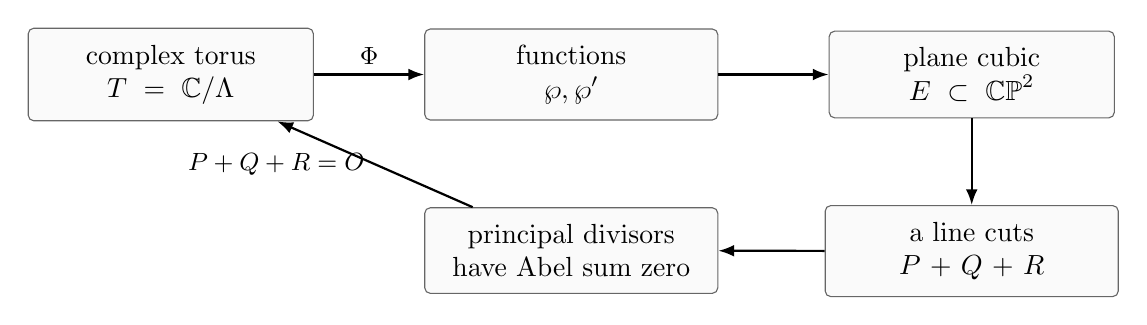
\begin{tikzpicture}[node distance=1.2cm]
  \node[visualnode, text width=3.2cm] (torus) {complex torus\\\(T=\C/\Lambda\)};
  \node[visualnode, text width=3.3cm, right=1.4cm of torus] (wp) {functions\\\(\wp,\wp'\)};
  \node[visualnode, text width=3.2cm, right=1.4cm of wp] (cubic) {plane cubic\\\(E\subset\CP^2\)};
  \node[visualnode, text width=3.3cm, below=1.1cm of wp] (div) {principal divisors\\have Abel sum zero};
  \node[visualnode, text width=3.3cm, below=1.1cm of cubic] (line) {a line cuts\\\(P+Q+R\)};
  \draw[arrow] (torus) -- node[above, labelnode] {\(\Phi\)} (wp);
  \draw[arrow] (wp) -- (cubic);
  \draw[arrow] (line) -- (div);
  \draw[arrow] (div) -- node[left, labelnode] {\(P+Q+R=O\)} (torus);
  \draw[arrow] (cubic) -- (line);
\end{tikzpicture}
\end{center}

\begin{keyidea}{Main conclusion}
If a line meets the cubic in three points \(P,Q,R\), counted with
intersection multiplicity, then those three points add to zero in the group
law transported from the torus:
\[
P+Q+R=O.
\]
Solving for \(P+Q\) gives
\[
P+Q=-R.
\]
Geometrically, this means: draw the line through \(P\) and \(Q\), take the
third intersection \(R\), then reflect \(R\) across the \(x\)-axis.
\end{keyidea}

\section{Where the Midterm and Final Exam Material Enters}

The argument is not just about elliptic curves.  It uses many of the
structural tools from the exams.

\subsection{From the Midterm}

\begin{enumerate}
\item \textbf{Differential forms and Stokes' theorem.}
The midterm emphasized that integral theorems are best understood as
statements about differential forms.  The residue theorem on compact
Riemann surfaces is another global Stokes-type statement.

\item \textbf{Cauchy--Green and residues.}
The proof that residues are global obstructions is the same philosophy:
local singular data must satisfy a global sum condition.

\item \textbf{The torus as a quotient.}
The midterm computed geometric invariants of a real torus and a complex
torus.  In the present notes the complex torus
\[
T=\C/\Lambda
\]
is the source of the group law.

\item \textbf{Euler characteristic of a torus.}
The midterm showed that the torus has Euler characteristic \(0\).  For a
compact Riemann surface,
\[
\chi=2-2g,
\]
so the complex torus has genus \(g=1\).  This is exactly the genus needed
for elliptic curves.
\end{enumerate}

\subsection{From the Final}

\begin{enumerate}
\item \textbf{Compact Riemann surfaces and meromorphic maps.}
The final used the fact that nonconstant holomorphic maps between compact
Riemann surfaces are finite branched coverings.  The functions \(\wp\) and
\(\wp'\) are meromorphic functions on a compact Riemann surface, namely
\(\C/\Lambda\).

\item \textbf{Principal divisors have degree zero.}
The final proved this using the logarithmic derivative \(df/f\).  That is
the first half of the Abel sum law.

\item \textbf{Riemann--Roch.}
On a genus-one surface, Riemann--Roch predicts exactly the dimensions that
force the functions \(1,\wp,\wp'\) to be the natural coordinate functions.

\item \textbf{The torus and \(\wp\).}
The final problem on \(\wp\) derived
\[
(\wp')^2=4\wp^3-g_2\wp-g_3.
\]
This is precisely the equation of the plane cubic.
\end{enumerate}

\begin{keyidea}{Exam-to-lecture bridge}
The midterm supplies the geometric and differential-form intuition.
The final supplies the compact Riemann surface tools.  Together they explain
why the algebraic-looking chord--tangent rule is actually forced by complex
analysis.
\end{keyidea}

\section{The Complex Torus}

\subsection{Lattices}

\begin{definition}
A \emph{lattice} in \(\C\) is a subgroup
\[
\Lambda=\Z\omega_1+\Z\omega_2
\]
where \(\omega_1,\omega_2\in\C\) are linearly independent over \(\R\).
Equivalently,
\[
\frac{\omega_1}{\omega_2}\notin\R.
\]
\end{definition}

The condition of real-linear independence means that the two periods span a
parallelogram of nonzero area in the complex plane.

\[
P_\Lambda
=
\{s\omega_1+t\omega_2:0\leq s,t\leq1\}.
\]

\begin{center}
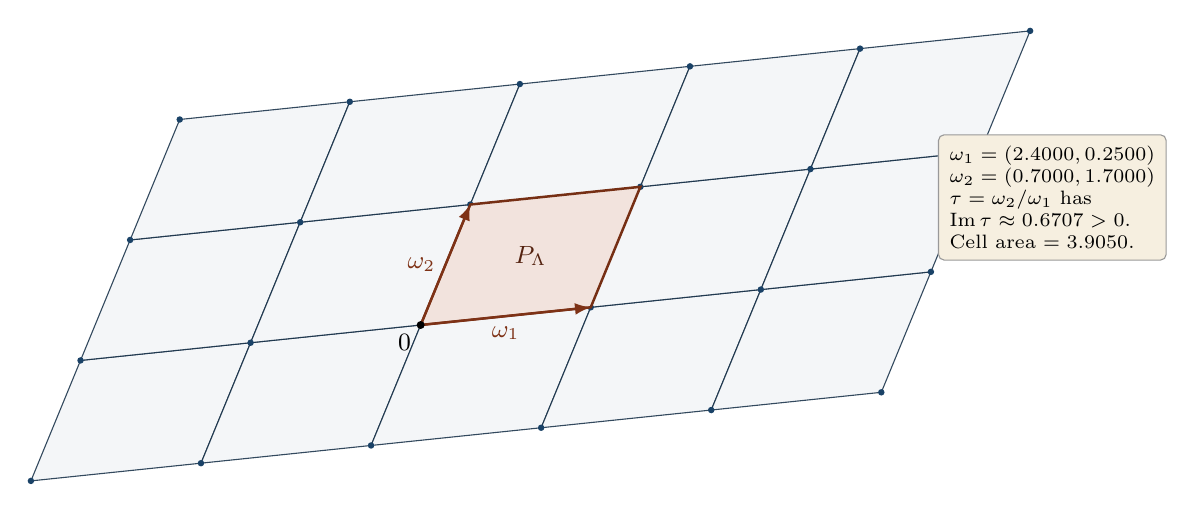
\begin{tikzpicture}[scale=0.9, every node/.style={font=\small}]
  % Lattice basis vectors (from sagemath/coords.tex)
  \pgfmathsetmacro{\axa}{\latwax}
  \pgfmathsetmacro{\aya}{\latway}
  \pgfmathsetmacro{\bxb}{\latwbx}
  \pgfmathsetmacro{\byb}{\latwby}
  % Tile the plane with lattice translates
  \foreach \i in {-2,-1,0,1,2}{
    \foreach \j in {-1,0,1}{
      \pgfmathsetmacro{\xa}{\i*\axa+\j*\bxb}
      \pgfmathsetmacro{\ya}{\i*\aya+\j*\byb}
      \pgfmathsetmacro{\xb}{(\i+1)*\axa+\j*\bxb}
      \pgfmathsetmacro{\yb}{(\i+1)*\aya+\j*\byb}
      \pgfmathsetmacro{\xc}{(\i+1)*\axa+(\j+1)*\bxb}
      \pgfmathsetmacro{\yc}{(\i+1)*\aya+(\j+1)*\byb}
      \pgfmathsetmacro{\xd}{\i*\axa+(\j+1)*\bxb}
      \pgfmathsetmacro{\yd}{\i*\aya+(\j+1)*\byb}
      \draw[draw=formteal!55!black, fill=formteal!6, line width=0.4pt, opacity=0.85]
        (\xa,\ya) -- (\xb,\yb) -- (\xc,\yc) -- (\xd,\yd) -- cycle;
    }
  }
  % Lattice points
  \foreach \i in {-2,-1,0,1,2,3}{
    \foreach \j in {-1,0,1,2}{
      \pgfmathsetmacro{\xx}{\i*\axa+\j*\bxb}
      \pgfmathsetmacro{\yy}{\i*\aya+\j*\byb}
      \fill[formteal!85!black] (\xx,\yy) circle (1.3pt);
    }
  }
  % Highlight the fundamental parallelogram at origin
  \draw[draw=formrust!70!black, fill=formrust!15, line width=0.9pt]
    (0,0) -- (\latwax,\latway) -- (\latsxc,\latsyc) -- (\latwbx,\latwby) -- cycle;
  \draw[-{Latex[length=2mm]}, thick, formrust!75!black] (0,0) -- (\latwax,\latway)
    node[midway, below] {$\omega_1$};
  \draw[-{Latex[length=2mm]}, thick, formrust!75!black] (0,0) -- (\latwbx,\latwby)
    node[midway, left] {$\omega_2$};
  \fill[black] (0,0) circle (1.6pt) node[below left] {$0$};
  \node[formrust!50!black] at (\latcellcx,\latcellcy) {$P_\Lambda$};
  % Annotation: sage-verified facts
  \node[draw=black!40, rounded corners=2pt, fill=formivory, align=left,
        inner sep=4pt, anchor=west, font=\scriptsize] at (7.3,1.8)
    {$\omega_1=\latomegaone$\\
     $\omega_2=\latomegatwo$\\
     $\tau=\omega_2/\omega_1$ has\\$\operatorname{Im}\tau\approx 0.6707>0$.\\
     Cell area $=3.9050$.};
\end{tikzpicture}
\end{center}

\subsection{The Quotient Surface}

Define an equivalence relation on \(\C\) by
\[
z\sim w
\quad\Longleftrightarrow\quad
z-w\in\Lambda.
\]
The quotient is
\[
T=\C/\Lambda.
\]
A point of \(T\) is an equivalence class
\[
[z]=z+\Lambda.
\]

The quotient map is
\[
\pi:\C\to\C/\Lambda,\qquad z\mapsto [z].
\]

Because the transition maps are translations, the complex coordinate \(z\)
on \(\C\) gives local holomorphic coordinates on the quotient.  Thus
\(\C/\Lambda\) is a compact Riemann surface.

\begin{center}
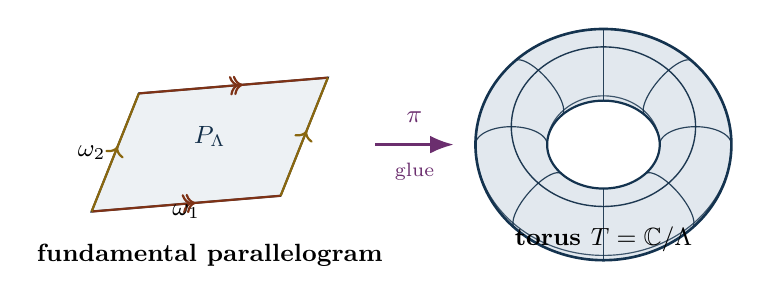
\begin{tikzpicture}[scale=1.0, every node/.style={font=\small}]
  % Left: fundamental parallelogram with side identifications
  \begin{scope}
    \draw[draw=formteal!55!black, fill=formteal!8, line width=0.7pt]
      (0,0) -- (2.4,0.2) -- (3.0,1.7) -- (0.6,1.5) -- cycle;
    % Side identification arrows (double-arrow markers)
    \draw[postaction={decorate, decoration={markings, mark=at position 0.55 with {\arrow[draw=formrust!75!black]{>}}, mark=at position 0.5 with {\arrow[draw=formrust!75!black, shift={(2pt,0)}]{>}}}}, formrust!75!black, line width=0.8pt] (0,0) -- (2.4,0.2);
    \draw[postaction={decorate, decoration={markings, mark=at position 0.55 with {\arrow[draw=formrust!75!black]{>}}, mark=at position 0.5 with {\arrow[draw=formrust!75!black, shift={(2pt,0)}]{>}}}}, formrust!75!black, line width=0.8pt] (0.6,1.5) -- (3.0,1.7);
    \draw[postaction={decorate, decoration={markings, mark=at position 0.55 with {\arrow[draw=formgold!75!black]{>}}}}, formgold!75!black, line width=0.8pt] (0,0) -- (0.6,1.5);
    \draw[postaction={decorate, decoration={markings, mark=at position 0.55 with {\arrow[draw=formgold!75!black]{>}}}}, formgold!75!black, line width=0.8pt] (2.4,0.2) -- (3.0,1.7);
    % Annotations
    \node at (1.2,0.0) {$\omega_1$};
    \node at (0.0,0.75) {$\omega_2$};
    \node[formteal!60!black] at (1.5,0.95) {$P_\Lambda$};
    \node at (1.5,-0.55) {\textbf{fundamental parallelogram}};
  \end{scope}
  % Arrow with quotient
  \draw[-{Latex[length=3mm]}, formplum, line width=1pt] (3.6,0.85) -- (4.6,0.85);
  \node[formplum] at (4.1,1.2) {$\pi$};
  \node[formplum, font=\scriptsize] at (4.1,0.5) {glue};
  % Right: precise torus rendered from sage
  \begin{scope}[xshift=6.5cm, yshift=0.85cm, scale=0.65]
    \drawprecisetorus
    \node at (0,-1.85) {\textbf{torus }$T=\C/\Lambda$};
  \end{scope}
\end{tikzpicture}
\end{center}

\subsection{The Group Law}

The complex plane is an abelian group under addition.  Since \(\Lambda\) is a
subgroup, the quotient inherits an abelian group law:
\[
[u]+[v]=[u+v].
\]

\begin{proposition}
The formula
\[
[u]+[v]=[u+v]
\]
is well-defined on \(\C/\Lambda\).
\end{proposition}

\begin{proof}
Suppose
\[
u'\equiv u\pmod{\Lambda},
\qquad
v'\equiv v\pmod{\Lambda}.
\]
Then
\[
u'=u+\lambda_1,\qquad v'=v+\lambda_2
\]
for some \(\lambda_1,\lambda_2\in\Lambda\).  Hence
\[
u'+v'=u+v+(\lambda_1+\lambda_2).
\]
Since \(\Lambda\) is a subgroup, \(\lambda_1+\lambda_2\in\Lambda\).  Therefore
\[
[u'+v']=[u+v].
\]
So the operation does not depend on the representatives.
\end{proof}

The identity element is
\[
0_T=[0],
\]
and the inverse of \([z]\) is
\[
-[z]=[-z].
\]

\begin{center}
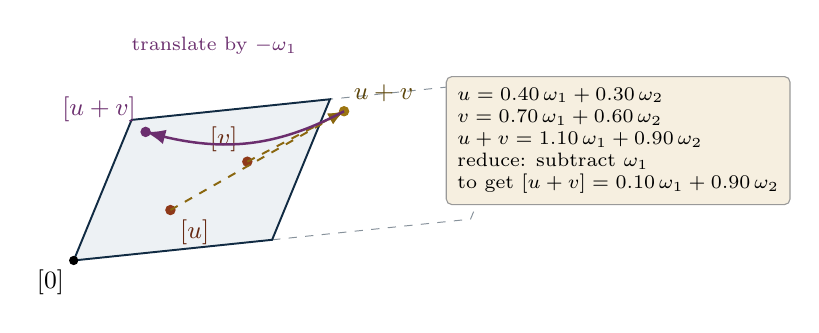
\begin{tikzpicture}[scale=1.05, every node/.style={font=\small}]
  % Fundamental parallelogram with sage-verified geometry
  \draw[draw=formteal!55!black, fill=formteal!8, line width=0.7pt]
    (0,0) -- (\latwax,\latway) -- (\latsxc,\latsyc) -- (\latwbx,\latwby) -- cycle;
  % Adjacent translate (where u+v lands)
  \draw[draw=formteal!45!black, dashed, line width=0.35pt, opacity=0.5]
    (\latwax,\latway) -- (2*\latwax,2*\latway)
    -- ({2*\latwax+\latwbx},{2*\latway+\latwby})
    -- (\latsxc,\latsyc);
  % Two points u, v (sage-computed: u = 0.40*w1 + 0.30*w2, v = 0.70*w1 + 0.60*w2)
  \fill[formrust!85!black] (\grupux,\grupuy) circle (1.8pt);
  \node[formrust!60!black, below right] at (\grupux,\grupuy) {$[u]$};
  \fill[formrust!85!black] (\grupvx,\grupvy) circle (1.8pt);
  \node[formrust!60!black, above left] at (\grupvx,\grupvy) {$[v]$};
  % u+v lifted (outside P_Lambda since the barycentric a=1.1)
  \fill[formgold!85!black] (\grupsumx,\grupsumy) circle (1.8pt);
  \node[formgold!50!black, above right] at (\grupsumx,\grupsumy) {$u+v$};
  \draw[-{Latex[length=2mm]}, draw=formgold!75!black, line width=0.7pt, dashed]
    (\grupux,\grupuy) -- (\grupsumx,\grupsumy);
  \draw[-{Latex[length=2mm]}, draw=formgold!75!black, line width=0.7pt, dashed]
    (\grupvx,\grupvy) -- (\grupsumx,\grupsumy);
  % Reduced representative (inside P_Lambda) via subtracting omega_1
  \fill[formplum] (\grupredx,\grupredy) circle (1.8pt);
  \node[formplum, above left, font=\small] at (\grupredx,\grupredy) {$[u+v]$};
  \draw[-{Latex[length=2.5mm]}, draw=formplum, line width=0.9pt]
    (\grupsumx,\grupsumy) to[bend left=22] (\grupredx,\grupredy);
  \node[formplum, font=\scriptsize] at (1.7,2.6) {translate by $-\omega_1$};
  % Origin
  \fill[black] (0,0) circle (1.6pt) node[below left] {$[0]$};
  % Annotation with sage-verified arithmetic
  \node[draw=black!40, rounded corners=2pt, fill=formivory, align=left, anchor=west,
        inner sep=4pt, font=\scriptsize] at (4.5,1.45)
    {$u=0.40\,\omega_1+0.30\,\omega_2$\\
     $v=0.70\,\omega_1+0.60\,\omega_2$\\
     $u+v=1.10\,\omega_1+0.90\,\omega_2$\\
     reduce: subtract $\omega_1$\\
     to get $[u+v]=0.10\,\omega_1+0.90\,\omega_2$};
\end{tikzpicture}
\end{center}

\subsection{The Torus as a Product of Circles}

The abstract group law \([u]+[v]=[u+v]\) has a concrete geometric
realization that makes abelianness transparent.

\medskip
\noindent\textbf{The circle group.}\quad
The unit circle
\[
S^1 = \{z\in\C : |z|=1\} = \{e^{i\theta}:\theta\in\R\}
\]
is an abelian group under \emph{complex multiplication}:
\[
e^{i\alpha}\cdot e^{i\beta} = e^{i(\alpha+\beta)}.
\]
Commutativity holds because \(\alpha+\beta=\beta+\alpha\) in \(\R\).
The exponential map
\[
\exp_{2\pi}:\R\to S^1,\qquad t\mapsto e^{2\pi it},
\]
is a surjective group homomorphism with \(\ker\exp_{2\pi}=\Z\).  By the
first isomorphism theorem,
\[
\R/\Z\;\cong\; S^1.
\]
Thus the circle is the real line \emph{folded into itself}: each unit
interval \([n, n{+}1)\) is wrapped onto \(S^1\) by angle \(\theta=2\pi
t\), and the group law becomes angle addition modulo \(2\pi\).

\begin{proposition}[Torus \(\cong\) product of circles]
\label{prop:s1xs1}
Let \(\Lambda=\Z\omega_1+\Z\omega_2\).  The map
\[
\Psi:\C/\Lambda\longrightarrow S^1\times S^1,
\qquad
[s\,\omega_1+t\,\omega_2]\longmapsto \bigl(e^{2\pi is},\,e^{2\pi it}\bigr)
\]
is an isomorphism of topological groups.
\end{proposition}

\begin{proof}
Because \(\omega_1,\omega_2\) are linearly independent over \(\R\), every
\(z\in\C\) has a unique decomposition \(z=s\omega_1+t\omega_2\) with
\(s,t\in\R\).  The real-linear map
\[
\phi:\R^2\to\C,\qquad (s,t)\mapsto s\omega_1+t\omega_2
\]
is an isomorphism of real vector spaces and sends \(\Z^2\) onto
\(\Lambda\), so it induces an isomorphism of abelian groups
\(\R^2/\Z^2\xrightarrow{\;\sim\;}\C/\Lambda\).  Composing with the
coordinate-wise exponential
\[
\R^2/\Z^2 = (\R/\Z)\times(\R/\Z)
\;\xrightarrow{\;(t_1,t_2)\,\mapsto\,(e^{2\pi it_1},\,e^{2\pi it_2})\;}
\;S^1\times S^1
\]
defines \(\Psi\).

\noindent\textit{Group homomorphism.}\quad
Write \([z_k]=[s_k\omega_1+t_k\omega_2]\) for \(k=1,2\).  Then
\begin{align*}
\Psi\bigl([z_1]+[z_2]\bigr)
&= \Psi\bigl([(s_1{+}s_2)\omega_1+(t_1{+}t_2)\omega_2]\bigr)\\
&= \bigl(e^{2\pi i(s_1+s_2)},\;e^{2\pi i(t_1+t_2)}\bigr)\\
&= \bigl(e^{2\pi is_1}{\cdot}e^{2\pi is_2},\;
           e^{2\pi it_1}{\cdot}e^{2\pi it_2}\bigr)
 = \Psi([z_1])\cdot\Psi([z_2]).
\end{align*}

\noindent\textit{Injectivity.}\quad
\(\Psi([z])=(1,1)\) forces \(e^{2\pi is}=e^{2\pi it}=1\), so
\(s,t\in\Z\), hence \(z=s\omega_1+t\omega_2\in\Lambda\) and
\([z]=[0]\).

\noindent\textit{Surjectivity.}\quad
Given any \((e^{2\pi is},e^{2\pi it})\in S^1\times S^1\), the class
\([s\omega_1+t\omega_2]\) maps to it.

\noindent\textit{Topological isomorphism.}\quad
Both \(\C/\Lambda\) and \(S^1\times S^1\) are compact Hausdorff spaces,
and \(\Psi\) is continuous (the exponential is continuous), so a
continuous bijection between compact Hausdorff spaces is automatically a
homeomorphism.
\end{proof}

\begin{corollary}\label{cor:torus-abelian-s1}
\(T=\C/\Lambda\) is an abelian group.
\end{corollary}

\begin{proof}
Since complex multiplication is commutative (\(wz=zw\) for all
\(w,z\in\C\)), the circle \(S^1\) is an abelian group.  A direct product
of abelian groups is abelian, so \(S^1\times S^1\) is abelian.  The
isomorphism \(\Psi\) therefore forces \(\C/\Lambda\) to be abelian.
\end{proof}

\begin{keyidea}{Why commutativity is obvious from the circle picture}
A class \([z]=[s\omega_1+t\omega_2]\) corresponds to the pair of points
\((e^{2\pi is}, e^{2\pi it})\) on two copies of the unit circle: one
tracking position along the \(\omega_1\)-direction, the other along
\(\omega_2\).  Adding two classes means \emph{rotating each circle
independently}:
\[
(e^{2\pi is_1},e^{2\pi it_1})\cdot(e^{2\pi is_2},e^{2\pi it_2})
= (e^{2\pi i(s_1+s_2)},\;e^{2\pi i(t_1+t_2)}).
\]
Since rotation by \(\alpha\) then by \(\beta\) is the same as rotation by
\(\beta\) then by \(\alpha\) (addition of real numbers commutes), the
group law is automatically commutative.  The two copies of \(S^1\) are
the two independent ``winding directions'' on the torus.
\end{keyidea}

\subsection{Genus One}

Topologically, the quotient of a parallelogram by identifying opposite sides
is a torus.  The midterm computation gives
\[
\chi(T)=0.
\]
For a compact connected Riemann surface of genus \(g\),
\[
\chi=2-2g.
\]
Thus
\[
0=2-2g,
\qquad
g=1.
\]

This genus-one fact is crucial.  It is why Riemann--Roch has the especially
simple form used below.

\section{Elliptic Functions as Meromorphic Functions on the Torus}

\subsection{Periodic Functions}

A meromorphic function \(f\) on \(\C\) is called \(\Lambda\)-periodic, or
\emph{elliptic with respect to \(\Lambda\)}, if
\[
f(z+\lambda)=f(z)
\qquad
\text{for all }\lambda\in\Lambda.
\]

Such a function descends to a meromorphic function on \(T=\C/\Lambda\),
because the value of \(f(z)\) depends only on the class \([z]\).

\[
\begin{array}{ccc}
\C & \xrightarrow{\ f\ } & \CP^1\\
\downarrow & & \\
\C/\Lambda &&
\end{array}
\]

Conversely, every meromorphic function on \(T\) pulls back to a
\(\Lambda\)-periodic meromorphic function on \(\C\).

\subsection{Why There Are No Nonconstant Holomorphic Functions}

The torus \(T\) is compact.  Therefore every holomorphic function
\[
T\to\C
\]
is constant by the maximum modulus principle.  Equivalently, every
\(\Lambda\)-periodic entire function on \(\C\) is constant.

Thus nonconstant functions on \(T\) must be meromorphic and must have poles.
The first question is:

\begin{quote}
How small can the pole divisor of a nonconstant meromorphic function on a
torus be?
\end{quote}

Riemann--Roch answers this.

\section{Divisors, Principal Divisors, and Logarithmic Derivatives}

\subsection{Orders}

Let \(X\) be a Riemann surface and let \(f\) be a nonzero meromorphic
function.  In a local coordinate \(t\) centered at \(p\), we can write
\[
f(t)=t^m u(t),
\]
where \(u\) is holomorphic and \(u(0)\neq0\).  The integer \(m\) is the order
of \(f\) at \(p\):
\[
\ord_p(f)=m.
\]

\begin{itemize}
\item If \(m>0\), then \(f\) has a zero of order \(m\) at \(p\).
\item If \(m=0\), then \(f\) is nonzero and finite at \(p\).
\item If \(m<0\), then \(f\) has a pole of order \(-m\) at \(p\).
\end{itemize}

\subsection{Divisors}

The divisor of \(f\) is
\[
(f)=\sum_{p\in X}\ord_p(f)\,p.
\]
Only finitely many coefficients are nonzero when \(X\) is compact.

The degree of a divisor
\[
D=\sum_p n_p p
\]
is
\[
\degdiv D=\sum_p n_p.
\]

A divisor of the form \((f)\) is called \emph{principal}.

\subsection{Principal Divisors Have Degree Zero}

The final exam proved the following result.

\begin{proposition}
If \(X\) is compact and \(f\) is a nonzero meromorphic function on \(X\), then
\[
\degdiv(f)=0.
\]
\end{proposition}

\begin{proof}
Consider the logarithmic derivative
\[
\frac{df}{f}.
\]
Near \(p\), write
\[
f=t^m u(t),
\qquad u(0)\neq0.
\]
Then
\[
\frac{df}{f}
=
\frac{d(t^m u)}{t^m u}
=
m\frac{dt}{t}+\frac{du}{u}.
\]
The second term is holomorphic at \(p\).  Therefore
\[
\Res_p\left(\frac{df}{f}\right)=m=\ord_p(f).
\]
By the residue theorem on a compact Riemann surface,
\[
\sum_p\Res_p\left(\frac{df}{f}\right)=0.
\]
Hence
\[
\sum_p\ord_p(f)=0,
\]
which is exactly
\[
\degdiv(f)=0.
\]
\end{proof}

\begin{keyidea}{What degree zero means}
A meromorphic function on a compact Riemann surface has as many zeros as
poles, counted with multiplicity.  This is the divisor version of the
argument principle.
\end{keyidea}

\section{Riemann--Roch on a Genus-One Surface}

\subsection{\texorpdfstring{The Spaces \(L(D)\)}{The Spaces L(D)}}

For a divisor \(D\) on a compact Riemann surface \(X\), define
\[
L(D)=
\{f\in\M(X):(f)+D\geq0\}\cup\{0\}.
\]
The condition \((f)+D\geq0\) means that the poles of \(f\) are bounded by
the positive part of \(D\), and that \(f\) has required zeros where \(D\) has
negative coefficients.

For example, if \(D=nO\) with \(n\geq0\), then
\[
L(nO)
\]
is the space of meromorphic functions whose only possible pole is at \(O\)
and whose pole order at \(O\) is at most \(n\).

\subsection{The Canonical Divisor of a Torus}

On \(T=\C/\Lambda\), the differential \(dz\) is translation-invariant:
\[
d(z+\lambda)=dz.
\]
Therefore \(dz\) descends to a nowhere-vanishing holomorphic \(1\)-form on
the quotient torus.  Hence its divisor is zero:
\[
(dz)=0.
\]
So the canonical divisor is linearly equivalent to \(0\).

\subsection{Riemann--Roch}

For a compact Riemann surface of genus \(g\), Riemann--Roch says
\[
\ell(D)-\ell(K-D)=\deg D+1-g,
\]
where
\[
\ell(D)=\dim_\C L(D)
\]
and \(K\) is a canonical divisor.

On a torus, \(g=1\) and \(K\sim0\).  Therefore
\[
\ell(D)-\ell(-D)=\deg D.
\]

For \(D=nO\) with \(n>0\), the divisor \(-nO\) has negative degree.  Thus
\[
L(-nO)=0,
\]
because a nonzero meromorphic function cannot have a divisor of total degree
positive enough to offset a negative-degree condition.  Hence
\[
\ell(nO)=n
\qquad
(n\geq1).
\]

\subsection{Consequences}

For \(n=1\),
\[
\ell(O)=1.
\]
Thus
\[
L(O)=\C.
\]
There is no nonconstant meromorphic function on a torus with only a simple
pole at one point.

For \(n=2\),
\[
\ell(2O)=2.
\]
The constants account for one dimension, so there is one new nonconstant
function with a double pole at \(O\).  This function is the Weierstrass
\(\wp\)-function, after a standard normalization.

For \(n=3\),
\[
\ell(3O)=3.
\]
A natural basis is
\[
1,\quad \wp,\quad \wp'.
\]

\begin{center}
\begin{tabular}{c|c|c|c}
Divisor & Dimension & Typical basis & Meaning\\
\hline
\(O\) & \(1\) & \(1\) & no simple-pole function\\
\(2O\) & \(2\) & \(1,\wp\) & first nonconstant function\\
\(3O\) & \(3\) & \(1,\wp,\wp'\) & projective embedding data
\end{tabular}
\end{center}

\begin{keyidea}{Why \(\wp\) and \(\wp'\) are inevitable}
Riemann--Roch says that the first nonconstant meromorphic function on a
complex torus appears with a double pole.  Its derivative has a triple pole.
Thus the first three natural functions are
\[
1,\qquad \wp,\qquad \wp'.
\]
These are exactly the functions needed to map the torus to a plane cubic.
\end{keyidea}

\section{The Weierstrass \texorpdfstring{\(\wp\)}{wp}-Function}

\subsection{Definition and Basic Shape}

For a lattice \(\Lambda\), the Weierstrass function is
\[
\wp(z)
=
\frac{1}{z^2}
+
\sum_{\lambda\in\Lambda\setminus\{0\}}
\left(
\frac{1}{(z-\lambda)^2}
-
\frac{1}{\lambda^2}
\right).
\]

The subtraction of \(1/\lambda^2\) makes the series converge normally on
compact subsets away from the lattice.  The function is meromorphic on
\(\C\), with a double pole at each lattice point.

It is \(\Lambda\)-periodic:
\[
\wp(z+\lambda)=\wp(z).
\]
It is also even:
\[
\wp(-z)=\wp(z).
\]
Therefore its derivative is odd:
\[
\wp'(-z)=-\wp'(z).
\]

\begin{center}
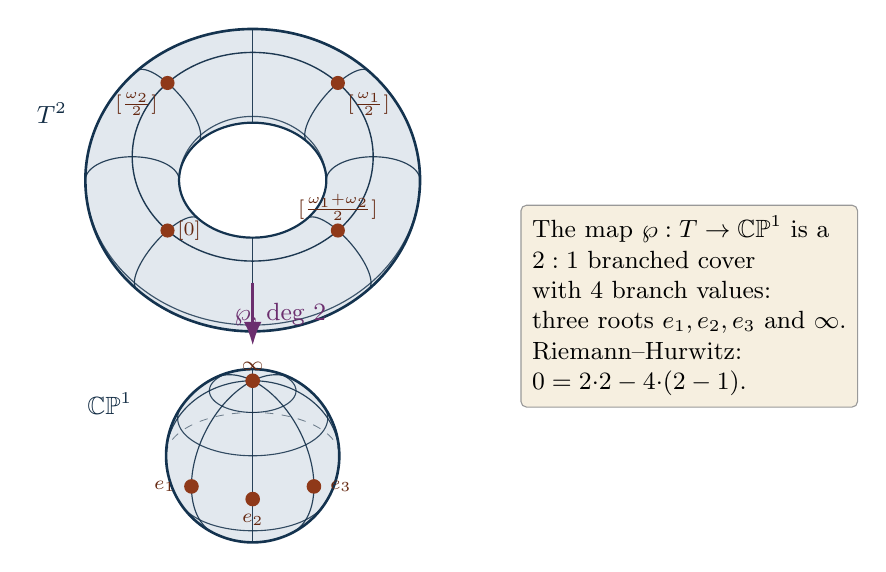
\begin{tikzpicture}[scale=1.0, every node/.style={font=\small}]
  % Top: precise torus with the four 2-torsion (half-lattice) points marked
  % at sage-verified visible-surface positions on the donut.
  \begin{scope}[yshift=2.0cm, scale=0.85]
    \drawprecisetorus
    % Half-lattice markers (visible-surface positions from 09_torus_markers.sage)
    \fill[formrust!85!black] (\torusMarkhalfsumx,\torusMarkhalfsumy) circle (3pt);
    \node[formrust!60!black, above, font=\scriptsize]
      at (\torusMarkhalfsumx,\torusMarkhalfsumy) {$[\tfrac{\omega_1+\omega_2}{2}]$};
    \fill[formrust!85!black] (\torusMarkzerox,\torusMarkzeroy) circle (3pt);
    \node[formrust!60!black, below right, font=\scriptsize]
      at (\torusMarkzerox,\torusMarkzeroy) {$[\tfrac{\omega_1}{2}]$};
    \fill[formrust!85!black] (\torusMarkhalftwox,\torusMarkhalftwoy) circle (3pt);
    \node[formrust!60!black, below left, font=\scriptsize]
      at (\torusMarkhalftwox,\torusMarkhalftwoy) {$[\tfrac{\omega_2}{2}]$};
    \fill[formrust!85!black] (\torusMarkhalfonex,\torusMarkhalfoney) circle (3pt);
    \node[formrust!60!black, right, font=\scriptsize]
      at (\torusMarkhalfonex,\torusMarkhalfoney) {$[0]$};
    \node[formteal!55!black] at (-3.0,1.0) {$T^2$};
  \end{scope}
  % Map arrow
  \draw[-{Latex[length=3mm]}, formplum, line width=1.1pt] (0,0.7) -- (0,-0.1);
  \node[formplum] at (0.35,0.3) {$\wp$, deg 2};
  % Bottom: precise sphere CP^1 rendered by 10_sphere_render.sage.
  % Three roots e_1, e_2, e_3 are placed on the visible front of the
  % equator (sin v < 0 portion: v in (pi, 2 pi)); infinity is the
  % north pole at the top.
  \begin{scope}[yshift=-1.5cm, scale=1.1]
    \drawprecisesphere
    % Branch values (rust for distinguished points, matching the torus
    % marker style at top); the labels use the same teal as the surface.
    \fill[formrust!85!black] (\sphereNorthx,\sphereNorthy) circle (2.4pt);
    \node[formrust!60!black, above, font=\scriptsize]
      at (\sphereNorthx,\sphereNorthy) {$\infty$};
    % Three roots on visible front of the equator (v = 5pi/4, 3pi/2, 7pi/4)
    % Their 2D projections (R=1, gamma=30 deg):
    %   v=5pi/4: (-0.707, -0.354)
    %   v=3pi/2: ( 0.000, -0.500)
    %   v=7pi/4: ( 0.707, -0.354)
    \fill[formrust!85!black] (-0.707,-0.354) circle (2.4pt);
    \node[formrust!60!black, left, font=\scriptsize] at (-0.78,-0.354) {$e_1$};
    \fill[formrust!85!black] (0,-0.500) circle (2.4pt);
    \node[formrust!60!black, below, font=\scriptsize] at (0,-0.56) {$e_2$};
    \fill[formrust!85!black] (0.707,-0.354) circle (2.4pt);
    \node[formrust!60!black, right, font=\scriptsize] at (0.78,-0.354) {$e_3$};
    \node[formteal!55!black] at (-1.65,0.6) {$\CP^1$};
  \end{scope}
  % Caption box
  \node[draw=black!40, rounded corners=2pt, fill=formivory, align=left, anchor=west,
        inner sep=4pt] at (3.4,0.4)
    {The map $\wp:T\to\CP^1$ is a\\$2:1$ branched cover\\
     with $4$ branch values:\\
     three roots $e_1,e_2,e_3$ and $\infty$.\\
     Riemann--Hurwitz:\\
     $0=2{\cdot}2-4{\cdot}(2-1)$.};
\end{tikzpicture}
\end{center}

\subsection{Laurent Expansions}

Near \(z=0\), \(\wp\) has the Laurent expansion
\[
\wp(z)=
\frac{1}{z^2}
a_2z^2+a_4z^4+a_6z^6+\cdots.
\]
There is no \(z^{-1}\) term because \(\wp\) has a double pole with zero
residue.  There are no odd powers because \(\wp\) is even.

Differentiating gives
\[
\wp'(z)
=
-\frac{2}{z^3}
2a_2z
4a_4z^3
6a_6z^5+\cdots.
\]
Thus \(\wp'\) has a triple pole at the origin and is odd.

\subsection{The Differential Equation}

The final exam derived the algebraic relation between \(\wp\) and \(\wp'\).
Let us spell out the computation.

Start with
\[
\wp(z)
=
z^{-2}+a_2z^2+a_4z^4+O(z^6),
\]
so
\[
\wp'(z)
=
-2z^{-3}+2a_2z+4a_4z^3+O(z^5).
\]
Then
\[
(\wp')^2
=
4z^{-6}-8a_2z^{-2}-16a_4+O(z^2),
\]
and
\[
4\wp^3
=
4z^{-6}+12a_2z^{-2}+12a_4+O(z^2).
\]
Hence
\[
(\wp')^2-4\wp^3
=
-20a_2z^{-2}-28a_4+O(z^2).
\]

Choose constants
\[
g_2=20a_2,
\qquad
g_3=28a_4.
\]
Then
\[
F(z)=(\wp')^2-4\wp^3+g_2\wp+g_3
\]
has no pole at \(z=0\).  Since \(F\) is elliptic, its only possible poles are
at lattice points.  By periodicity the same cancellation occurs at every
lattice point.  Therefore \(F\) is holomorphic on the compact torus
\(\C/\Lambda\), so it is constant.

The expansion also shows that the constant is \(0\).  Therefore
\[
\boxed{
(\wp')^2=4\wp^3-g_2\wp-g_3.
}
\]

\begin{keyidea}{The birth of the cubic}
The equation
\[
(\wp')^2=4\wp^3-g_2\wp-g_3
\]
is not guessed.  It is forced because a carefully chosen combination of
\(\wp\) and \(\wp'\) has no poles, hence must be constant on the compact
torus.
\end{keyidea}

\subsection{Minimality}

The same final-exam argument shows that \(\wp'\) has degree \(2\) over
\(\C(\wp)\).  The relation above says \(\wp'\) satisfies
\[
T^2-(4\wp^3-g_2\wp-g_3)=0.
\]
It remains to see that \(\wp'\notin\C(\wp)\).

If \(\wp'=R(\wp)\) for a rational function \(R\), then \(R(\wp)\) would be
even, since \(\wp\) is even.  But \(\wp'\) is odd and nonzero.  This is
impossible.  Thus the quadratic relation is minimal.

\section{The \texorpdfstring{\(\wp\)}{wp}-Embedding of the Torus}

\subsection{The Projective Map}

Define
\[
\Phi:T=\C/\Lambda\longrightarrow\CP^2
\]
by
\[
\Phi([z])=[\wp(z):\wp'(z):1]
\]
for \(z\notin\Lambda\).

Because \(\wp\) and \(\wp'\) are periodic, this is well-defined on the
quotient.  Because they satisfy the differential equation, the image lies on
\[
E:\quad Y^2Z=4X^3-g_2XZ^2-g_3Z^3.
\]
Indeed, in the affine chart \(Z=1\), the equation becomes
\[
y^2=4x^3-g_2x-g_3,
\]
and substituting \(x=\wp(z)\), \(y=\wp'(z)\) gives exactly the differential
equation.

\begin{center}
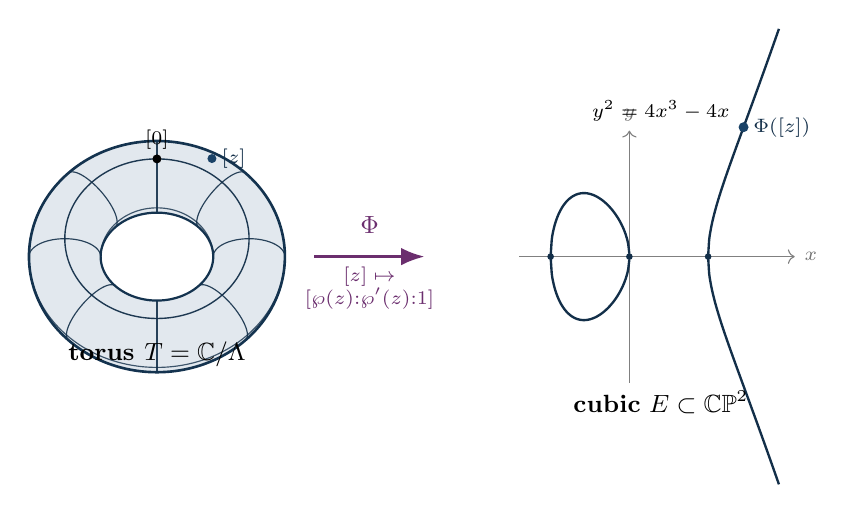
\begin{tikzpicture}[scale=1.0, every node/.style={font=\small}]
  % Left: precise torus rendered from sage with two visible markers
  \begin{scope}[scale=0.65]
    \drawprecisetorus
    \fill[formteal!85!black] (\torusMarkZx,\torusMarkZy) circle (2.5pt);
    \node[formteal!60!black, right, font=\scriptsize] at (\torusMarkZx,\torusMarkZy) {$[z]$};
    \fill[black] (\torusMarkOriginx,\torusMarkOriginy) circle (2.5pt);
    \node[font=\scriptsize, above] at (\torusMarkOriginx,\torusMarkOriginy) {$[0]$};
    \node at (0,-1.9) {\textbf{torus }$T=\C/\Lambda$};
  \end{scope}
  % Arrow representing the embedding
  \draw[-{Latex[length=3mm]}, formplum, line width=1.1pt] (2.0,0) -- (3.4,0);
  \node[formplum] at (2.7,0.4) {$\Phi$};
  \node[formplum, font=\scriptsize, align=center] at (2.7,-0.4) {$[z]\mapsto$\\$[\wp(z){:}\wp'(z){:}1]$};
  % Right: real elliptic curve y^2 = 4x^3 - 4x (sage-computed roots {-1,0,1})
  \begin{scope}[xshift=6.0cm]
    \draw[->, black!50, line width=0.4pt] (-1.4,0) -- (2.1,0) node[right, black!55, font=\scriptsize] {$x$};
    \draw[->, black!50, line width=0.4pt] (0,-1.6) -- (0,1.6) node[above, black!55, font=\scriptsize] {$y$};
    \draw[draw=formteal!60!black, line width=0.85pt, smooth, samples=70, variable=\x, domain=-1.0:0.0]
      plot (\x, {0.65*sqrt(max(0,4*\x*\x*\x-4*\x))});
    \draw[draw=formteal!60!black, line width=0.85pt, smooth, samples=70, variable=\x, domain=-1.0:0.0]
      plot (\x, {-0.65*sqrt(max(0,4*\x*\x*\x-4*\x))});
    \draw[draw=formteal!60!black, line width=0.85pt, smooth, samples=70, variable=\x, domain=1.0:1.9]
      plot (\x, {0.65*sqrt(max(0,4*\x*\x*\x-4*\x))});
    \draw[draw=formteal!60!black, line width=0.85pt, smooth, samples=70, variable=\x, domain=1.0:1.9]
      plot (\x, {-0.65*sqrt(max(0,4*\x*\x*\x-4*\x))});
    \foreach \rt in {\rooteone,\rootetwo,\rootethree}
      \fill[formteal!60!black] (\rt,0) circle (1.2pt);
    % Sample image of a torus point Phi([z]) at x=1.45 (sage chord-Q point)
    \fill[formteal!85!black] (\chordQx,{0.65*\chordQy}) circle (1.8pt);
    \node[formteal!60!black, right, font=\scriptsize] at (\chordQx,{0.65*\chordQy}) {$\Phi([z])$};
    \node at (0.4,-1.85) {\textbf{cubic} $E\subset\CP^2$};
    \node[font=\scriptsize] at (0.4,1.85) {$y^2=4x^3-4x$};
  \end{scope}
\end{tikzpicture}
\end{center}

\subsection{Extension at the Origin}

At \(z=0\), both \(\wp\) and \(\wp'\) have poles, so the affine formula is
not meaningful.  But the projective formula has a limit.

Near \(0\),
\[
\wp(z)=z^{-2}+O(z^2),
\qquad
\wp'(z)=-2z^{-3}+O(z).
\]
Thus
\[
[\wp(z):\wp'(z):1]
=
[z^3\wp(z):z^3\wp'(z):z^3].
\]
As \(z\to0\),
\[
z^3\wp(z)\to0,\qquad
z^3\wp'(z)\to-2,\qquad
z^3\to0.
\]
Therefore
\[
\lim_{z\to0}[\wp(z):\wp'(z):1]
=[0:-2:0]=[0:1:0].
\]

So we define
\[
\Phi(0)=[0:1:0]=O.
\]

\begin{proposition}
The map
\[
\Phi:T\to E,\qquad
\Phi(z)=[\wp(z):\wp'(z):1],
\]
with \(\Phi(0)=O=[0:1:0]\), is a holomorphic map from the torus to the
projective cubic \(E\).
\end{proposition}

\subsection{The Point at Infinity}

The projective cubic is
\[
Y^2Z=4X^3-g_2XZ^2-g_3Z^3.
\]
Set \(Z=0\).  Then the equation becomes
\[
0=4X^3.
\]
Hence
\[
X=0.
\]
The only projective point with \(X=0\) and \(Z=0\) is
\[
[0:1:0].
\]
Thus \(O=[0:1:0]\) is the unique point at infinity on \(E\).

\subsection{Why This Map Is the Right Embedding}

The functions \(1,\wp,\wp'\) form a basis of \(L(3O)\).  The associated
projective map is
\[
z\longmapsto [1:\wp(z):\wp'(z)]
\]
up to a reordering of coordinates.  We use
\[
[\wp(z):\wp'(z):1]
\]
so that the affine chart \(Z=1\) has coordinates \(x=\wp(z)\),
\(y=\wp'(z)\).

Riemann--Roch explains why \(L(3O)\) is large enough:
\[
\ell(3O)=3.
\]
Three independent sections give a map to \(\CP^2\).  The single algebraic
relation among them is the cubic equation.

\subsection{Injectivity, Briefly}

One can show:

\begin{lemma}
If \(\wp(z)=\wp(w)\), then
\[
w\equiv z
\quad\text{or}\quad
w\equiv -z
\pmod{\Lambda}.
\]
\end{lemma}

This reflects the fact that the map
\[
T\to\CP^1,\qquad z\mapsto\wp(z)
\]
has degree \(2\), and its two generic fibers are \(\{z,-z\}\).

If also
\[
\wp'(z)=\wp'(w),
\]
then the possibility \(w\equiv -z\) forces
\[
\wp'(z)=\wp'(-z)=-\wp'(z),
\]
so \(\wp'(z)=0\).  At such a branch point, \(z\equiv -z\), meaning
\[
2z\in\Lambda.
\]
Thus the two alternatives coincide on the torus.  Therefore \(\Phi\) is
injective.

\begin{remark}
The full proof that \(\Phi\) is a biholomorphism from \(T\) onto the smooth
cubic \(E\) can be obtained by combining injectivity, compactness, and the
fact that a nonconstant holomorphic map between compact Riemann surfaces is
a finite branched covering.  Since \(T\) is compact and \(E\) is Hausdorff,
a continuous bijective holomorphic map \(T\to E\) is a biholomorphism.
\end{remark}

\section{\texorpdfstring{Inverses Become Reflection Across the \(x\)-Axis}{Inverses Become Reflection Across the x-Axis}}

The inverse on the torus is
\[
z\mapsto -z.
\]
Because
\[
\wp(-z)=\wp(z),
\qquad
\wp'(-z)=-\wp'(z),
\]
we get
\[
\Phi(-z)
=
[\wp(-z):\wp'(-z):1]
=
[\wp(z):-\wp'(z):1].
\]

In affine coordinates, if
\[
P=(x,y)=(\wp(z),\wp'(z)),
\]
then
\[
-P=(x,-y).
\]

\begin{center}
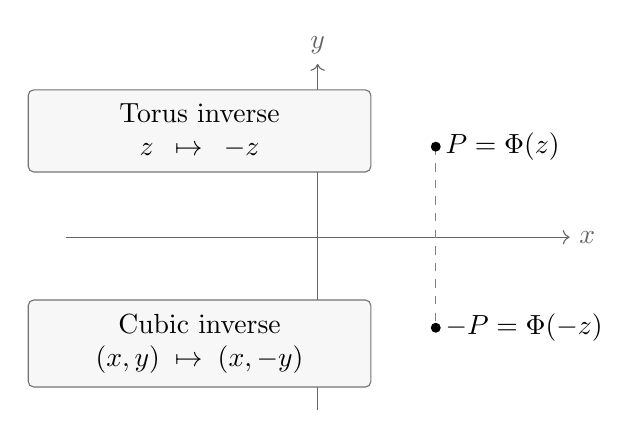
\begin{tikzpicture}[scale=1.0]
  \draw[->, black!60] (-3.2,0) -- (3.2,0) node[right] {\(x\)};
  \draw[->, black!60] (0,-2.2) -- (0,2.2) node[above] {\(y\)};
  \coordinate (P) at (1.5,1.15);
  \coordinate (N) at (1.5,-1.15);
  \draw[dashed, gray] (P) -- (N);
  \fill[black] (P) circle (1.8pt) node[right] {\(P=\Phi(z)\)};
  \fill[black] (N) circle (1.8pt) node[right] {\(-P=\Phi(-z)\)};
  \node[note, text width=4cm] at (-1.5,1.35)
    {Torus inverse\\\(z\mapsto -z\)};
  \node[note, text width=4cm] at (-1.5,-1.35)
    {Cubic inverse\\\((x,y)\mapsto(x,-y)\)};
\end{tikzpicture}
\end{center}

\begin{keyidea}{Why reflection appears}
Reflection across the \(x\)-axis is not an extra convention.  It is exactly
the torus inverse \(z\mapsto -z\) written in the coordinates
\[
x=\wp(z),\qquad y=\wp'(z).
\]
\end{keyidea}

\begin{center}
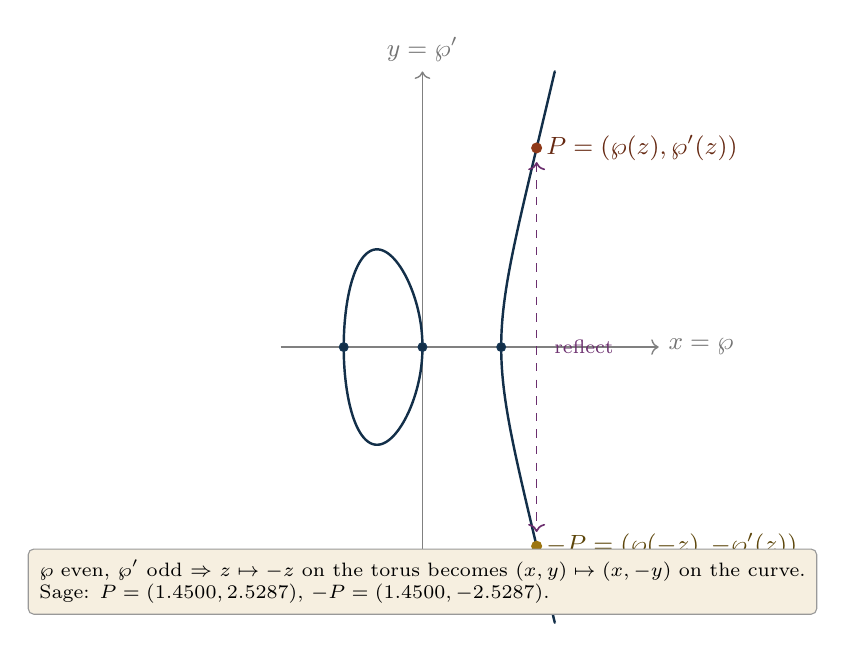
\begin{tikzpicture}[scale=1.0, every node/.style={font=\small}]
  % Axes
  \draw[->, black!50, line width=0.5pt] (-1.8,0) -- (3.0,0) node[right, black!55] {$x=\wp$};
  \draw[->, black!50, line width=0.5pt] (0,-3.4) -- (0,3.5) node[above, black!55] {$y=\wp'$};
  % Sage curve y^2 = 4x^3 - 4x with roots -1, 0, 1
  % Curve arcs and branch points from sagemath/12_curve_sample.sage
  \drawprecisecurve
  % Sage roots
  \foreach \rt in {\rooteone,\rootetwo,\rootethree}
    \fill[formteal!60!black] (\rt,0) circle (1.3pt);
  % Point P (sage-sampled at x=1.45) and -P
  \fill[formrust!85!black] (\chordQx,\chordQy) circle (2pt);
  \node[formrust!60!black, right] at (\chordQx,\chordQy) {$P=(\wp(z),\wp'(z))$};
  \fill[formgold!85!black] (\chordQx,{-\chordQy}) circle (2pt);
  \node[formgold!50!black, right] at (\chordQx,{-\chordQy}) {$-P=(\wp(-z),-\wp'(z))$};
  \draw[<->, draw=formplum, line width=0.6pt, dashed]
    (\chordQx,{\chordQy-0.18}) -- (\chordQx,{-\chordQy+0.18});
  \node[formplum, font=\scriptsize, anchor=west] at ({\chordQx+0.10},0) {reflect};
  \node[draw=black!40, rounded corners=2pt, fill=formivory, align=left, anchor=south,
        inner sep=4pt, font=\scriptsize] at (0.0,-3.4)
    {$\wp$ even, $\wp'$ odd $\Rightarrow$ $z\mapsto-z$ on the torus becomes
     $(x,y)\mapsto(x,-y)$ on the curve.\\
     Sage: $P=(\chordQx,\chordQy)$, $-P=(\chordQx,{-\chordQy})$.};
\end{tikzpicture}
\end{center}

\section{Abel's Sum Law on a Torus}

\subsection{Statement}

The central divisor fact is the genus-one form of Abel's theorem.

\begin{theorem}[Abel sum law for elliptic functions]
Let \(F\) be a nonzero meromorphic function on
\[
T=\C/\Lambda.
\]
Write its divisor as
\[
(F)=\sum_j n_j[z_j],
\]
where \(z_j\in\C\) are representatives of points on \(T\).  Then
\[
\sum_j n_j=0
\]
and
\[
\sum_j n_jz_j\in\Lambda.
\]
Equivalently,
\[
\sum_j n_j[z_j]=0
\]
in the group law of \(T\).
\end{theorem}

The first equation is the degree-zero property of principal divisors.  The
second equation says that zeros and poles also balance in the torus group
law.

\subsection{Proof of the Degree Condition}

Pull \(F\) back to a \(\Lambda\)-periodic meromorphic function on \(\C\).
Choose a fundamental parallelogram whose boundary contains no zeros or poles
of \(F\).  The logarithmic derivative
\[
\frac{F'}{F}\,dz
\]
is periodic.  By the residue theorem,
\[
\frac{1}{2\pi i}
\int_{\partial P_\Lambda}\frac{F'}{F}\,dz
=
\sum_j n_j.
\]
Opposite sides of the parallelogram cancel because \(F'/F\) is periodic.
Therefore the boundary integral is \(0\).  Hence
\[
\sum_j n_j=0.
\]

\subsection{Proof of the Abel-Sum Condition}

Now integrate
\[
z\frac{F'}{F}\,dz
\]
around the same fundamental parallelogram.  Its residues are
\[
\Res_{z_j}
\left(
z\frac{F'}{F}\,dz
\right)
=
n_jz_j.
\]
Therefore
\[
\frac{1}{2\pi i}
\int_{\partial P_\Lambda}
z\frac{F'}{F}\,dz
=
\sum_j n_jz_j.
\]

Unlike \(F'/F\), the function \(zF'/F\) is not periodic because of the
factor \(z\).  The opposite sides no longer cancel exactly.  The failure of
cancellation is a period.

Let the parallelogram have sides \(\omega_1\) and \(\omega_2\).  Since
\[
\frac{F'}{F}
\]
is periodic, the boundary integral reduces to
\[
\omega_1\int_{\text{one }\omega_2\text{-side}}\frac{F'}{F}\,dz
-
\omega_2\int_{\text{one }\omega_1\text{-side}}\frac{F'}{F}\,dz.
\]
Each side integral is a change of a branch of \(\log F\).  Since
\(F(z+\omega_k)=F(z)\), that change is an integer multiple of \(2\pi i\).
Thus
\[
\int_{\partial P_\Lambda}z\frac{F'}{F}\,dz
\in
2\pi i\,\Lambda.
\]
Dividing by \(2\pi i\) gives
\[
\sum_j n_jz_j\in\Lambda.
\]

\begin{keyidea}{Meaning of Abel's sum law}
A principal divisor on a torus is not only degree zero.  Its weighted sum of
points is also zero in the group law of the torus.
\[
(F)=\sum n_jp_j
\quad\Longrightarrow\quad
\sum n_jp_j=0\quad\text{in }T.
\]
\end{keyidea}

\section{Lines on the Cubic Give Principal Divisors}

\subsection{A Projective Line}

A projective line in \(\CP^2\) is given by a homogeneous linear equation
\[
\ell(X,Y,Z)=aX+bY+cZ.
\]
Restricting \(\ell\) to the cubic \(E\) gives a meromorphic function only
after we divide by another homogeneous function of the same degree.  The
standard comparison function is \(Z\), the line at infinity.

Thus
\[
\frac{\ell}{Z}
\]
is a meromorphic function on \(E\).

\subsection{Intersection Divisors}

If the line \(L=\{\ell=0\}\) meets \(E\) in points
\[
P,Q,R,
\]
counted with multiplicity, then
\[
\divisor_0(\ell|_E)=P+Q+R.
\]
This is B\'ezout's theorem in the special case of a line and a cubic: a
degree-one curve and a degree-three curve meet in \(3\) points, counted with
intersection multiplicity.

\subsection{The Divisor of the Line at Infinity}

The line at infinity is
\[
Z=0.
\]
On
\[
E:\quad Y^2Z=4X^3-g_2XZ^2-g_3Z^3,
\]
we already saw that \(Z=0\) meets \(E\) only at
\[
O=[0:1:0].
\]
The multiplicity is \(3\).

Here is a local check.  Work in the chart \(Y=1\) near \(O\).  Put
\[
u=\frac{X}{Y},
\qquad
v=\frac{Z}{Y}.
\]
Then \(O\) is \((u,v)=(0,0)\), and the cubic equation becomes
\[
v=4u^3-g_2uv^2-g_3v^3.
\]
Near \((0,0)\), this equation implies
\[
v=4u^3+\text{higher-order terms}.
\]
Thus \(u\) is a local parameter and
\[
Z/Y=v
\]
vanishes to order \(3\) at \(O\).  Therefore
\[
\divisor_0(Z|_E)=3O.
\]

\subsection{The Principal Divisor Associated to a Line}

Since \(\ell/Z\) is a meromorphic function on \(E\), its divisor is
principal:
\[
\left(\frac{\ell}{Z}\right)
=
\divisor_0(\ell|_E)-\divisor_0(Z|_E).
\]
If
\[
L\cdot E=P+Q+R,
\]
then
\[
\boxed{
\left(\frac{\ell}{Z}\right)=P+Q+R-3O.
}
\]

\begin{keyidea}{The line divisor}
Every projective line cuts the cubic in a divisor linearly equivalent to
\(3O\):
\[
P+Q+R\sim3O.
\]
Equivalently,
\[
P+Q+R-3O
\]
is principal.
\end{keyidea}

\section{Transporting the Torus Group Law to the Cubic}

The \(\wp\)-embedding gives a biholomorphic identification
\[
\Phi:T=\C/\Lambda\longrightarrow E.
\]
We transport the torus group law to \(E\) by declaring
\[
P+_E Q
=
\Phi(u+v)
\]
whenever
\[
P=\Phi(u),
\qquad
Q=\Phi(v).
\]

The identity is
\[
O=\Phi(0)=[0:1:0].
\]
The inverse is
\[
-\Phi(u)=\Phi(-u).
\]
In affine coordinates this is
\[
-(x,y)=(x,-y).
\]

The question is:

\begin{quote}
Why does this transported group law coincide with the chord--tangent law?
\end{quote}

The answer is: because line divisors are principal and principal divisors
have Abel sum zero.

\section{Pictorial Dictionary: Torus Addition vs.\ Chord--Tangent}
\label{sec:dictionary}

The map \(\Phi:\C/\Lambda\to E\) is a group isomorphism.  Each addition on the
left corresponds to a chord--tangent construction on the right.  The three
figures below display this dictionary for the three structurally distinct
cases: adding the identity, adding two distinct nonopposite points, and
doubling a single point.

%-------------------------------------------------------------------
% Overview figure: lattice | torus | elliptic curve side-by-side.
% All geometry is computed by sagemath scripts:
%   lattice coords  -- 01_lattice.sage  -> coords_lattice.tex
%   torus rendering -- 08_torus_render.sage -> coords_torus.tex  (\drawprecisetorus)
%   curve sample    -- 12_curve_sample.sage -> coords_curve_sample.tex (\drawprecisecurve)
%-------------------------------------------------------------------
\begin{center}
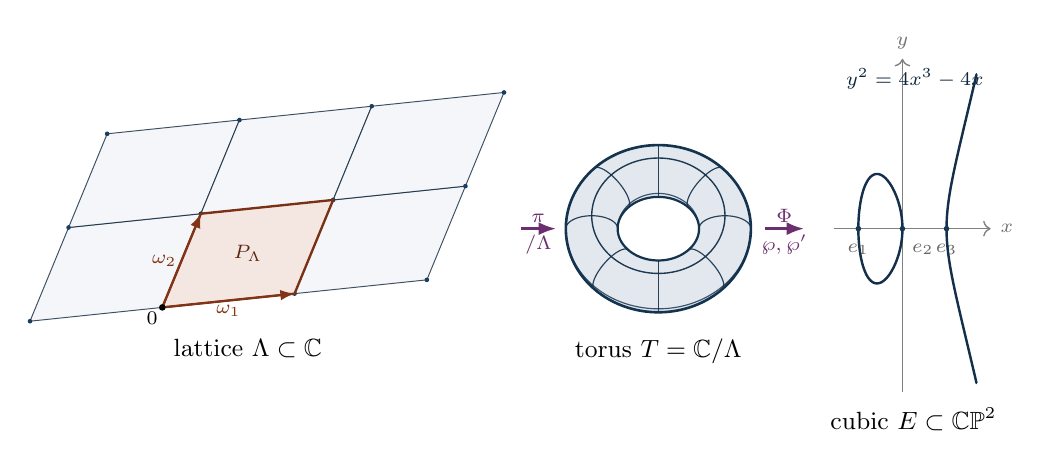
\begin{tikzpicture}[every node/.style={font=\small}]
  %=== Panel 1: Lattice Lambda ============================================
  % Scale 0.70: fundamental domain is 3.1*0.70 = 2.17 cm wide.
  % Tiles for i in {-1,0,1}, j in {0,1} (6 cells, 2 rows above x-axis).
  % Rightmost tile corner (i=1,j=1): (6.2,3.9)*0.70 = (4.34,2.73) cm in parent.
  \begin{scope}[scale=0.70]
    % Background lattice tiles
    \foreach \i in {-1,0,1}{
      \foreach \j in {0,1}{
        \pgfmathsetmacro{\xa}{\i*\latwax+\j*\latwbx}
        \pgfmathsetmacro{\ya}{\i*\latway+\j*\latwby}
        \pgfmathsetmacro{\xb}{(\i+1)*\latwax+\j*\latwbx}
        \pgfmathsetmacro{\yb}{(\i+1)*\latway+\j*\latwby}
        \pgfmathsetmacro{\xc}{(\i+1)*\latwax+(\j+1)*\latwbx}
        \pgfmathsetmacro{\yc}{(\i+1)*\latway+(\j+1)*\latwby}
        \pgfmathsetmacro{\xd}{\i*\latwax+(\j+1)*\latwbx}
        \pgfmathsetmacro{\yd}{\i*\latway+(\j+1)*\latwby}
        \draw[draw=formteal!50!black, fill=formteal!6, line width=0.35pt, opacity=0.80]
          (\xa,\ya) -- (\xb,\yb) -- (\xc,\yc) -- (\xd,\yd) -- cycle;
      }
    }
    % Lattice points
    \foreach \i in {-1,0,1,2}{
      \foreach \j in {0,1,2}{
        \pgfmathsetmacro{\xx}{\i*\latwax+\j*\latwbx}
        \pgfmathsetmacro{\yy}{\i*\latway+\j*\latwby}
        \fill[formteal!80!black] (\xx,\yy) circle (1.2pt);
      }
    }
    % Fundamental parallelogram (highlighted)
    \draw[draw=formrust!72!black, fill=formrust!13, line width=0.85pt]
      (0,0) -- (\latwax,\latway) -- (\latsxc,\latsyc) -- (\latwbx,\latwby) -- cycle;
    % Basis vectors with arrows
    \draw[-{Latex[length=1.8mm]}, formrust!78!black, line width=0.65pt]
      (0,0) -- (\latwax,\latway)
      node[midway, below, font=\scriptsize, inner sep=1.5pt] {$\omega_1$};
    \draw[-{Latex[length=1.8mm]}, formrust!78!black, line width=0.65pt]
      (0,0) -- (\latwbx,\latwby)
      node[midway, left, font=\scriptsize, inner sep=1.5pt] {$\omega_2$};
    \fill[black] (0,0) circle (1.7pt);
    \node[below left, inner sep=1.5pt, font=\scriptsize] at (0,0) {$0$};
    \node[formrust!55!black, font=\scriptsize]
      at (\latcellcx,\latcellcy) {$P_\Lambda$};
    % Caption (in scope coords, below domain)
    \node[font=\small, anchor=north] at ({(\latwax+\latwbx)/2},{\latway-0.65})
      {lattice $\Lambda\subset\C$};
  \end{scope}

  %=== Arrow: quotient map pi: C -> C/Lambda ==============================
  % Arrow placed between rightmost tile edge (~4.34 cm) and torus left edge.
  % Torus: xshift=6.30, scale=0.47 => left edge = 6.30 - 2.5*0.47 = 5.125 cm.
  \draw[-{Latex[length=2.2mm]}, formplum, line width=0.9pt] (4.55,1.0) -- (5.00,1.0);
  \node[formplum, above, font=\scriptsize, inner sep=2pt] at (4.775,1.0)
    {$\pi$};
  \node[formplum, below, font=\scriptsize, inner sep=2pt] at (4.775,1.0)
    {$/\Lambda$};

  %=== Panel 2: Torus T = C/Lambda ========================================
  % At scale 0.47: outer silhouette radius = 2.5*0.47 = 1.175 cm.
  % Scope center at parent (6.30, 1.0).
  \begin{scope}[xshift=6.30cm, yshift=1.0cm, scale=0.47]
    \drawprecisetorus
    \node[font=\small, anchor=north] at (0,-2.72)
      {torus $T=\C/\Lambda$};
  \end{scope}

  %=== Arrow: Weierstrass embedding Phi ===================================
  % Torus right edge = 6.30 + 2.5*0.47 = 7.475 cm.
  \draw[-{Latex[length=2.2mm]}, formplum, line width=0.9pt] (7.65,1.0) -- (8.15,1.0);
  \node[formplum, above, font=\scriptsize, inner sep=2pt] at (7.90,1.0)
    {$\Phi$};
  \node[formplum, below, font=\scriptsize, inner sep=2pt] at (7.90,1.0)
    {$\wp,\wp'$};

  %=== Panel 3: Elliptic curve E: y^2 = 4x^3 - 4x ========================
  % Scope center at parent (9.40, 1.0).
  % At scale 0.56: x in [-1.55, 1.69] maps to parent x in [8.532, 10.346].
  \begin{scope}[xshift=9.40cm, yshift=1.0cm, scale=0.56]
    % Axes
    \draw[->, black!50, line width=0.5pt]
      (-1.55,0) -- (2.00,0) node[right, black!55, font=\scriptsize] {$x$};
    \draw[->, black!50, line width=0.5pt]
      (0,-3.70) -- (0,3.85) node[above, black!55, font=\scriptsize] {$y$};
    % Root tick marks
    \draw[black!40, line width=0.4pt] (-1,-0.12) -- (-1,0.12);
    \draw[black!40, line width=0.4pt] ( 0,-0.12) -- ( 0,0.12);
    \draw[black!40, line width=0.4pt] ( 1,-0.12) -- ( 1,0.12);
    \node[black!60, below, font=\scriptsize] at (-1,-0.12) {$e_1$};
    \node[black!60, below right, font=\scriptsize] at (0,-0.12) {$e_2$};
    \node[black!60, below, font=\scriptsize] at (1,-0.12) {$e_3$};
    % Curve arcs from sage-computed coordinate lists
    \drawprecisecurve
    % Caption and equation label
    \node[font=\small, anchor=north] at (0.25,-3.85)
      {cubic $E\subset\CP^2$};
    \node[font=\scriptsize, formteal!50!black, anchor=north west] at (-1.50,3.85)
      {$y^2=4x^3-4x$};
  \end{scope}
\end{tikzpicture}
\end{center}

Throughout, the rust colour marks the input points, plum marks the
auxiliary line (chord, tangent, or vertical), teal marks the third
intersection \(R\), and gold marks the final result obtained by reflecting
\(R\) across the \(x\)-axis.

All coordinates in the figures below are computed in
\texttt{sagemath/11\_correspondence.sage}.  Each marker
\([w]=a\,\omega_1+b\,\omega_2\) is shown in three locations:
its position in the fundamental parallelogram \(P_\Lambda\); its embedded
3D position on the torus via \(u_t=2\pi b\), \(v_t=2\pi a\) (small-circle
/ big-circle angles, then orthographic projection at \(\theta=60^\circ\));
and the corresponding chord/tangent picture on \(E:y^2=4x^3-4x\).
Lattice coefficients \((a,b)\) are kept small enough that every embedded
marker passes the visibility check
\(-\cos u_t\sin v_t\cos\theta+\sin u_t\sin\theta>0\).

%-------------------------------------------------------------------
% Figure 1: Identity addition  P + O = P
%-------------------------------------------------------------------
\subsection{Identity element: \texorpdfstring{$P+O=P$}{P+O=P}}

On the torus, adding the identity \(0\) is the trivial translation
\([u]\mapsto[u]+0=[u]\).  Under \(\Phi\), the identity \(0\) maps to the
point at infinity \(O\), and the line through \(P\) and \(O\) is the
vertical line through \(P\); its third intersection with the cubic is
\(-P\), and reflecting \(-P\) across the \(x\)-axis recovers \(P\).

\begin{center}
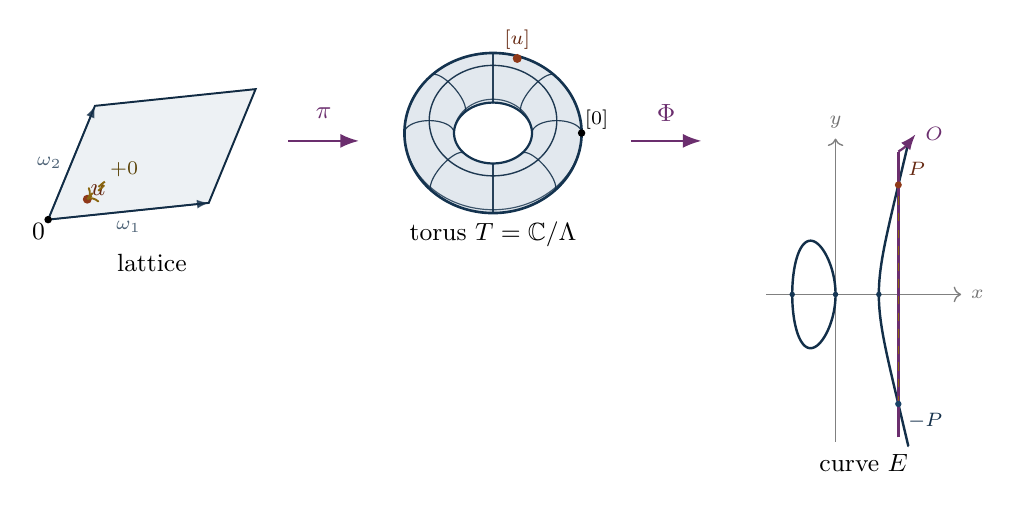
\begin{tikzpicture}[every node/.style={font=\small}]
  %--- Panel 1: lattice ---------------------------------------------------
  \begin{scope}[scale=0.85]
    \draw[draw=formteal!55!black, fill=formteal!8, line width=0.7pt]
      (0,0) -- (\latwax,\latway) -- (\latsxc,\latsyc) -- (\latwbx,\latwby) -- cycle;
    \draw[-{Latex[length=1.5mm]}, formteal!60!black, line width=0.5pt, opacity=0.75]
      (0,0) -- (\latwax,\latway) node[midway, below, font=\scriptsize] {$\omega_1$};
    \draw[-{Latex[length=1.5mm]}, formteal!60!black, line width=0.5pt, opacity=0.75]
      (0,0) -- (\latwbx,\latwby) node[midway, left, font=\scriptsize] {$\omega_2$};
    \fill[black] (\corOriginLx,\corOriginLy) circle (1.6pt);
    \node[anchor=north east, inner sep=1pt] at (\corOriginLx,\corOriginLy) {$0$};
    \fill[formrust!85!black] (\corULx,\corULy) circle (1.9pt);
    \node[formrust!60!black, above right, inner sep=1pt] at (\corULx,\corULy) {$u$};
    % "+0" loop indicator
    \draw[->, formgold!75!black, line width=0.7pt, dashed]
      (\corULx,\corULy) .. controls ({\corULx+0.35},{\corULy+0.42})
                       and ({\corULx+0.45},{\corULy+0.32}) .. (\corULx,\corULy);
    \node[formgold!50!black, font=\scriptsize] at ({\corULx+0.55},{\corULy+0.45}) {$+0$};
    \node[font=\small] at (1.55,-0.65) {lattice};
  \end{scope}
  %--- Arrow lattice -> torus ---------------------------------------------
  \draw[-{Latex[length=2.4mm]}, formplum, line width=0.9pt] (3.05,1.0) -- (3.95,1.0);
  \node[formplum] at (3.5,1.35) {$\pi$};
  %--- Panel 2: torus -----------------------------------------------------
  \begin{scope}[xshift=5.65cm, yshift=1.1cm, scale=0.45]
    \drawprecisetorus
    \fill[black] (\corOriginTx,\corOriginTy) circle (3.0pt);
    \node[anchor=south west, inner sep=1pt, font=\scriptsize] at (\corOriginTx,\corOriginTy) {$[0]$};
    \fill[formrust!85!black] (\corUTx,\corUTy) circle (3.6pt);
    \node[formrust!60!black, anchor=south, inner sep=1pt, font=\scriptsize]
      at ({\corUTx},{\corUTy+0.15}) {$[u]$};
    \node[font=\small] at (0,-2.85) {torus $T=\C/\Lambda$};
  \end{scope}
  %--- Arrow torus -> curve -----------------------------------------------
  \draw[-{Latex[length=2.4mm]}, formplum, line width=0.9pt] (7.4,1.0) -- (8.3,1.0);
  \node[formplum] at (7.85,1.35) {$\Phi$};
  %--- Panel 3: curve -----------------------------------------------------
  \begin{scope}[xshift=10.0cm, yshift=-0.95cm, scale=0.55]
    \draw[->, black!50, line width=0.5pt] (-1.6,0) -- (2.9,0) node[right, black!55, font=\scriptsize] {$x$};
    \draw[->, black!50, line width=0.5pt] (0,-3.4) -- (0,3.6) node[above, black!55, font=\scriptsize] {$y$};
    % Curve arcs and branch points from sagemath/12_curve_sample.sage
    \drawprecisecurve
    \draw[draw=formplum, line width=0.85pt] (\corCurveIDPx,-3.3) -- (\corCurveIDPx,3.3);
    \draw[dashed, line width=0.55pt, formgold!75!black]
      (\corCurveIDPx,-\corCurveIDPy) -- (\corCurveIDPx,\corCurveIDPy);
    \fill[formrust!85!black] (\corCurveIDPx,\corCurveIDPy) circle (2.3pt);
    \node[formrust!60!black, above right, font=\scriptsize] at (\corCurveIDPx,\corCurveIDPy) {$P$};
    \fill[formteal!85!black] (\corCurveIDPx,-\corCurveIDPy) circle (2.1pt);
    \node[formteal!60!black, below right, font=\scriptsize] at (\corCurveIDPx,-\corCurveIDPy) {$-P$};
    \draw[draw=formplum, line width=0.8pt, -{Latex[length=2mm]}]
      (\corCurveIDPx,3.3) to[bend right=14] ({\corCurveIDPx+0.4},3.7);
    \node[formplum, font=\scriptsize, right] at ({\corCurveIDPx+0.4},3.7) {$O$};
    \node[font=\small] at (0.65,-3.9) {curve $E$};
  \end{scope}
\end{tikzpicture}
\end{center}

\noindent\textit{Reading the figure.} On the lattice (left) the
self-loop at \(u\) records the trivial translation \(u+0=u\).  The same
points \([u],[0]\) appear at their embedded torus positions (middle)
via \((v_t,u_t)=(2\pi a,2\pi b)\).  On the curve (right) the chord
\(\overline{PO}\) is vertical; it meets \(E\) at \(P\), \(-P\), and
\(O\), so the chord-tangent rule says
\(P+O+(-P)=O\), i.e.\ \(P+O=P\).

%-------------------------------------------------------------------
% Figure 2: P + Q for two distinct points
%-------------------------------------------------------------------
\subsection{Two distinct points: \texorpdfstring{$P+Q$}{P+Q}}

On the torus, addition is just vector addition modulo \(\Lambda\): from
\([u]\) translate by \(v\) to reach the lifted sum \(u+v\), then reduce
modulo \(\Lambda\) back into \(P_\Lambda\).  On the cubic, draw the chord
through \(P\) and \(Q\); it meets \(E\) at a third point \(R\), and
reflecting \(R\) across the \(x\)-axis yields \(P+Q=-R\).

\begin{center}
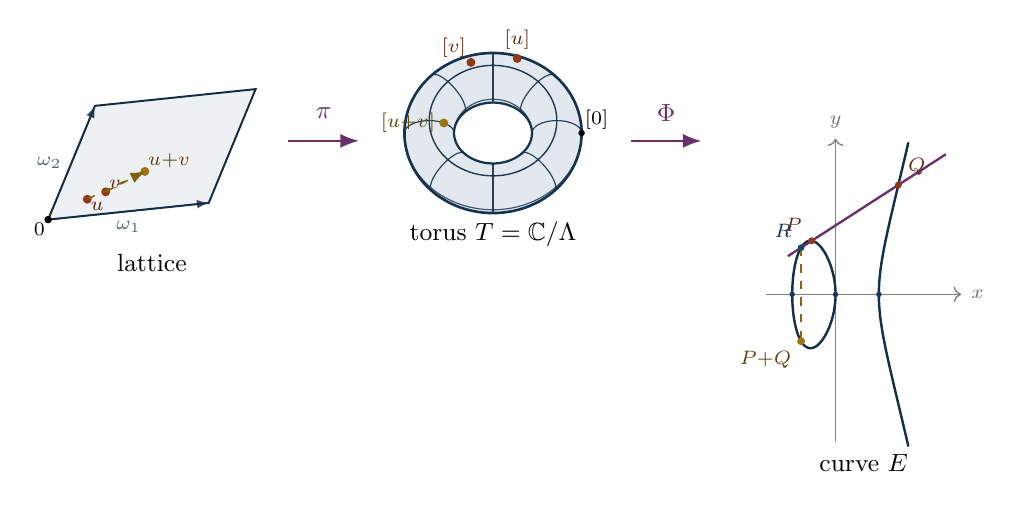
\begin{tikzpicture}[every node/.style={font=\small}]
  %--- Panel 1: lattice ---------------------------------------------------
  \begin{scope}[scale=0.85]
    \draw[draw=formteal!55!black, fill=formteal!8, line width=0.7pt]
      (0,0) -- (\latwax,\latway) -- (\latsxc,\latsyc) -- (\latwbx,\latwby) -- cycle;
    \draw[-{Latex[length=1.5mm]}, formteal!60!black, line width=0.5pt, opacity=0.75]
      (0,0) -- (\latwax,\latway) node[midway, below, font=\scriptsize] {$\omega_1$};
    \draw[-{Latex[length=1.5mm]}, formteal!60!black, line width=0.5pt, opacity=0.75]
      (0,0) -- (\latwbx,\latwby) node[midway, left, font=\scriptsize] {$\omega_2$};
    % Origin
    \fill[black] (\corOriginLx,\corOriginLy) circle (1.6pt)
      node[below left, inner sep=1pt, font=\scriptsize] {$0$};
    % u, v, sum
    \fill[formrust!85!black] (\corULx,\corULy) circle (1.9pt);
    \node[formrust!60!black, below right, inner sep=1pt, font=\scriptsize] at (\corULx,\corULy) {$u$};
    \fill[formrust!85!black] (\corVLx,\corVLy) circle (1.9pt);
    \node[formrust!60!black, above right, inner sep=1pt, font=\scriptsize] at (\corVLx,\corVLy) {$v$};
    \fill[formgold!85!black] (\corSumLiftLx,\corSumLiftLy) circle (1.9pt);
    \node[formgold!50!black, above right, inner sep=1pt, font=\scriptsize]
      at (\corSumLiftLx,\corSumLiftLy) {$u{+}v$};
    % Translation arrows from origin -> u -> u+v (forming a "+v" shift)
    \draw[-{Latex[length=1.8mm]}, draw=formgold!70!black, line width=0.55pt, dashed]
      (\corULx,\corULy) -- (\corSumLiftLx,\corSumLiftLy);
    \draw[-{Latex[length=1.8mm]}, draw=formgold!70!black, line width=0.55pt, dashed]
      (\corVLx,\corVLy) -- (\corSumLiftLx,\corSumLiftLy);
    \node[font=\small] at (1.55,-0.65) {lattice};
  \end{scope}
  %--- Arrow lattice -> torus ---------------------------------------------
  \draw[-{Latex[length=2.4mm]}, formplum, line width=0.9pt] (3.05,1.0) -- (3.95,1.0);
  \node[formplum] at (3.5,1.35) {$\pi$};
  %--- Panel 2: torus -----------------------------------------------------
  \begin{scope}[xshift=5.65cm, yshift=1.1cm, scale=0.45]
    \drawprecisetorus
    \fill[black] (\corOriginTx,\corOriginTy) circle (2.6pt);
    \node[anchor=south west, inner sep=1pt, font=\scriptsize] at (\corOriginTx,\corOriginTy) {$[0]$};
    \fill[formrust!85!black] (\corUTx,\corUTy) circle (3.6pt);
    \node[formrust!60!black, anchor=south, inner sep=1pt, font=\scriptsize]
      at ({\corUTx},{\corUTy+0.15}) {$[u]$};
    \fill[formrust!85!black] (\corVTx,\corVTy) circle (3.6pt);
    \node[formrust!60!black, anchor=south east, inner sep=1pt, font=\scriptsize]
      at ({\corVTx-0.05},{\corVTy+0.05}) {$[v]$};
    \fill[formgold!85!black] (\corSumRedTx,\corSumRedTy) circle (3.6pt);
    \node[formgold!50!black, anchor=east, inner sep=1pt, font=\scriptsize]
      at ({\corSumRedTx-0.15},{\corSumRedTy}) {$[u{+}v]$};
    \node[font=\small] at (0,-2.85) {torus $T=\C/\Lambda$};
  \end{scope}
  %--- Arrow torus -> curve -----------------------------------------------
  \draw[-{Latex[length=2.4mm]}, formplum, line width=0.9pt] (7.4,1.0) -- (8.3,1.0);
  \node[formplum] at (7.85,1.35) {$\Phi$};
  %--- Panel 3: curve -----------------------------------------------------
  \begin{scope}[xshift=10.0cm, yshift=-0.95cm, scale=0.55]
    \draw[->, black!50, line width=0.5pt] (-1.6,0) -- (2.9,0) node[right, black!55, font=\scriptsize] {$x$};
    \draw[->, black!50, line width=0.5pt] (0,-3.4) -- (0,3.6) node[above, black!55, font=\scriptsize] {$y$};
    % Curve arcs and branch points from sagemath/12_curve_sample.sage
    \drawprecisecurve
    \draw[draw=formplum, line width=0.85pt]
      (\corCurveCLeftx,\corCurveCLefty) -- (\corCurveCRightx,\corCurveCRighty);
    \draw[dashed, line width=0.55pt, formgold!75!black]
      (\corCurveCRx,\corCurveCRy) -- (\corCurveCSumx,\corCurveCSumy);
    \fill[formrust!85!black] (\corCurveCPx,\corCurveCPy) circle (2.3pt);
    \node[formrust!60!black, above left, font=\scriptsize] at (\corCurveCPx,\corCurveCPy) {$P$};
    \fill[formrust!85!black] (\corCurveCQx,\corCurveCQy) circle (2.3pt);
    \node[formrust!60!black, above right, font=\scriptsize] at (\corCurveCQx,\corCurveCQy) {$Q$};
    \fill[formteal!85!black] (\corCurveCRx,\corCurveCRy) circle (2.2pt);
    \node[formteal!60!black, above left, font=\scriptsize] at (\corCurveCRx,\corCurveCRy) {$R$};
    \fill[formgold!85!black] (\corCurveCSumx,\corCurveCSumy) circle (2.6pt);
    \node[formgold!50!black, below left, font=\scriptsize] at (\corCurveCSumx,\corCurveCSumy) {$P{+}Q$};
    \node[font=\small] at (0.65,-3.9) {curve $E$};
  \end{scope}
\end{tikzpicture}
\end{center}

\noindent\textit{Reading the figure.} The two dashed gold arrows on the
parallelogram show \(u\to u+v\) and \(v\to u+v\); under \(\pi\) those two
translates land at the same point \([u+v]\) on the torus.  The chord on
\(E\) then meets the cubic at a third point \(R\); reflecting gives
\(P+Q=-R\).  Numerically (from Sage): \(P=(\corCurveCPx,\corCurveCPy)\),
\(Q=(\corCurveCQx,\corCurveCQy)\), \(R=(\corCurveCRx,\corCurveCRy)\),
\(P+Q=(\corCurveCSumx,\corCurveCSumy)\).

%-------------------------------------------------------------------
% Figure 3: Doubling 2P (P = Q)
%-------------------------------------------------------------------
\subsection{Doubling a point: \texorpdfstring{$2P$}{2P}}

The doubling case is the limit of the chord rule as \(Q\to P\): the
chord becomes the tangent line at \(P\) with intersection multiplicity
\(2\) at \(P\).  On the torus, doubling \([u]\) is just
\([u]+[u]=[2u]\), the ordinary vector \(2u\) reduced modulo \(\Lambda\).

\begin{center}
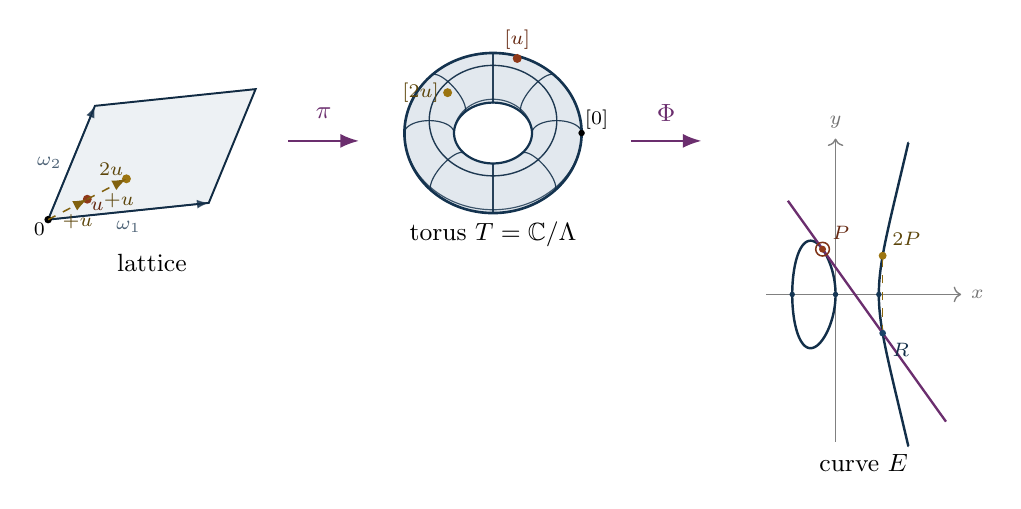
\begin{tikzpicture}[every node/.style={font=\small}]
  %--- Panel 1: lattice ---------------------------------------------------
  \begin{scope}[scale=0.85]
    \draw[draw=formteal!55!black, fill=formteal!8, line width=0.7pt]
      (0,0) -- (\latwax,\latway) -- (\latsxc,\latsyc) -- (\latwbx,\latwby) -- cycle;
    \draw[-{Latex[length=1.5mm]}, formteal!60!black, line width=0.5pt, opacity=0.75]
      (0,0) -- (\latwax,\latway) node[midway, below, font=\scriptsize] {$\omega_1$};
    \draw[-{Latex[length=1.5mm]}, formteal!60!black, line width=0.5pt, opacity=0.75]
      (0,0) -- (\latwbx,\latwby) node[midway, left, font=\scriptsize] {$\omega_2$};
    \fill[black] (\corOriginLx,\corOriginLy) circle (1.6pt)
      node[below left, inner sep=1pt, font=\scriptsize] {$0$};
    \fill[formrust!85!black] (\corULx,\corULy) circle (1.9pt);
    \node[formrust!60!black, below right, inner sep=1pt, font=\scriptsize] at (\corULx,\corULy) {$u$};
    \fill[formgold!85!black] (\corTwoURedLx,\corTwoURedLy) circle (1.9pt);
    \node[formgold!50!black, above left, inner sep=1pt, font=\scriptsize] at (\corTwoURedLx,\corTwoURedLy) {$2u$};
    % Two consecutive "+u" arrows
    \draw[-{Latex[length=1.8mm]}, draw=formgold!70!black, line width=0.55pt, dashed]
      (\corOriginLx,\corOriginLy) -- (\corULx,\corULy);
    \draw[-{Latex[length=1.8mm]}, draw=formgold!70!black, line width=0.55pt, dashed]
      (\corULx,\corULy) -- (\corTwoURedLx,\corTwoURedLy);
    \node[formgold!50!black, font=\scriptsize] at ({0.5*\corULx+0.15},{0.5*\corULy-0.18}) {$+u$};
    \node[formgold!50!black, font=\scriptsize] at ({(\corULx+\corTwoURedLx)/2+0.18},{(\corULy+\corTwoURedLy)/2-0.18}) {$+u$};
    \node[font=\small] at (1.55,-0.65) {lattice};
  \end{scope}
  %--- Arrow lattice -> torus ---------------------------------------------
  \draw[-{Latex[length=2.4mm]}, formplum, line width=0.9pt] (3.05,1.0) -- (3.95,1.0);
  \node[formplum] at (3.5,1.35) {$\pi$};
  %--- Panel 2: torus -----------------------------------------------------
  \begin{scope}[xshift=5.65cm, yshift=1.1cm, scale=0.45]
    \drawprecisetorus
    \fill[black] (\corOriginTx,\corOriginTy) circle (2.6pt);
    \node[anchor=south west, inner sep=1pt, font=\scriptsize] at (\corOriginTx,\corOriginTy) {$[0]$};
    \fill[formrust!85!black] (\corUTx,\corUTy) circle (3.6pt);
    \node[formrust!60!black, anchor=south, inner sep=1pt, font=\scriptsize]
      at ({\corUTx},{\corUTy+0.15}) {$[u]$};
    \fill[formgold!85!black] (\corTwoURedTx,\corTwoURedTy) circle (3.6pt);
    \node[formgold!50!black, anchor=east, inner sep=1pt, font=\scriptsize]
      at ({\corTwoURedTx-0.15},{\corTwoURedTy}) {$[2u]$};
    \node[font=\small] at (0,-2.85) {torus $T=\C/\Lambda$};
  \end{scope}
  %--- Arrow torus -> curve -----------------------------------------------
  \draw[-{Latex[length=2.4mm]}, formplum, line width=0.9pt] (7.4,1.0) -- (8.3,1.0);
  \node[formplum] at (7.85,1.35) {$\Phi$};
  %--- Panel 3: curve -----------------------------------------------------
  \begin{scope}[xshift=10.0cm, yshift=-0.95cm, scale=0.55]
    \draw[->, black!50, line width=0.5pt] (-1.6,0) -- (2.9,0) node[right, black!55, font=\scriptsize] {$x$};
    \draw[->, black!50, line width=0.5pt] (0,-3.4) -- (0,3.6) node[above, black!55, font=\scriptsize] {$y$};
    % Curve arcs and branch points from sagemath/12_curve_sample.sage
    \drawprecisecurve
    \draw[draw=formplum, line width=0.85pt]
      (\corCurveDLeftx,\corCurveDLefty) -- (\corCurveDRightx,\corCurveDRighty);
    \draw[dashed, line width=0.55pt, formgold!75!black]
      (\corCurveDRx,\corCurveDRy) -- (\corCurveDTwoPx,\corCurveDTwoPy);
    \fill[formrust!85!black] (\corCurveDPx,\corCurveDPy) circle (2.3pt);
    \draw[draw=formrust!75!black, line width=0.55pt] (\corCurveDPx,\corCurveDPy) circle (4.5pt);
    \node[formrust!60!black, above right, font=\scriptsize] at (\corCurveDPx,\corCurveDPy) {$P$};
    \fill[formteal!85!black] (\corCurveDRx,\corCurveDRy) circle (2.2pt);
    \node[formteal!60!black, below right, font=\scriptsize] at (\corCurveDRx,\corCurveDRy) {$R$};
    \fill[formgold!85!black] (\corCurveDTwoPx,\corCurveDTwoPy) circle (2.6pt);
    \node[formgold!50!black, above right, font=\scriptsize] at (\corCurveDTwoPx,\corCurveDTwoPy) {$2P$};
    \node[font=\small] at (0.65,-3.9) {curve $E$};
  \end{scope}
\end{tikzpicture}
\end{center}

\noindent\textit{Reading the figure.} Two consecutive \(+u\) translations on
the parallelogram give the lifted vector \(2u\); under \(\pi\) this lands at
\([2u]\) on the torus, marked in gold.  Under \(\Phi\) the marker \([u]\)
maps to \(P\), and the chord limit (i.e.\ tangent at \(P\)) hits the cubic
at \(R\); reflecting gives \(2P=-R\).  Numerically:
\(P=(\corCurveDPx,\corCurveDPy)\), tangent slope
\(m=\tfrac{12x_P^2-g_2}{2y_P}\),
\(R=(\corCurveDRx,\corCurveDRy)\),
\(2P=(\corCurveDTwoPx,\corCurveDTwoPy)\).

\begin{remark}
The three figures share the same colour code: rust for the input(s), plum
for the auxiliary line (vertical / chord / tangent), teal for the residual
intersection \(R\), and gold for the final result.  The single visual rule
shared by every case is:
\[
\boxed{\;
\text{points + line on }E\;\xrightarrow{\;\text{Vieta}\;} R
\;\xrightarrow{\;y\mapsto-y\;} R+(\text{stuff})=O,
\;\text{so result}=-R.
\;}
\]
\end{remark}

\section{The Chord Law: Distinct Points}

\subsection{Setup}

Let \(P,Q\in E\) be two distinct finite points with \(Q\neq -P\).  Let \(L\)
be the line through \(P\) and \(Q\).  Since \(L\) is not vertical in this
case, it meets the cubic in a third finite point \(R\).

Write
\[
P=\Phi(u),\qquad Q=\Phi(v),\qquad R=\Phi(w).
\]

The intersection divisor is
\[
L\cdot E=P+Q+R.
\]
Therefore
\[
\left(\frac{\ell}{Z}\right)=P+Q+R-3O.
\]

\subsection{Apply Abel's Sum Law}

Pull this principal divisor back to the torus.  Since \(O=\Phi(0)\), Abel's
sum law gives
\[
u+v+w-3\cdot0\equiv0\pmod{\Lambda}.
\]
Hence
\[
w\equiv-(u+v)\pmod{\Lambda}.
\]
Therefore
\[
R=\Phi(w)=\Phi(-(u+v)).
\]

But the torus sum of \(P\) and \(Q\) is
\[
P+_E Q=\Phi(u+v).
\]
Since inverse on the cubic is reflection,
\[
\Phi(u+v)=-\Phi(-(u+v)).
\]
Thus
\[
\boxed{
P+_E Q=-R.
}
\]

\subsection{Geometric Rule}

This is exactly the chord rule:

\begin{enumerate}
\item Draw the line through \(P\) and \(Q\).
\item Let \(R\) be the third intersection with the cubic.
\item Reflect \(R\) across the \(x\)-axis.
\item The reflected point is \(P+Q\).
\end{enumerate}

\begin{center}
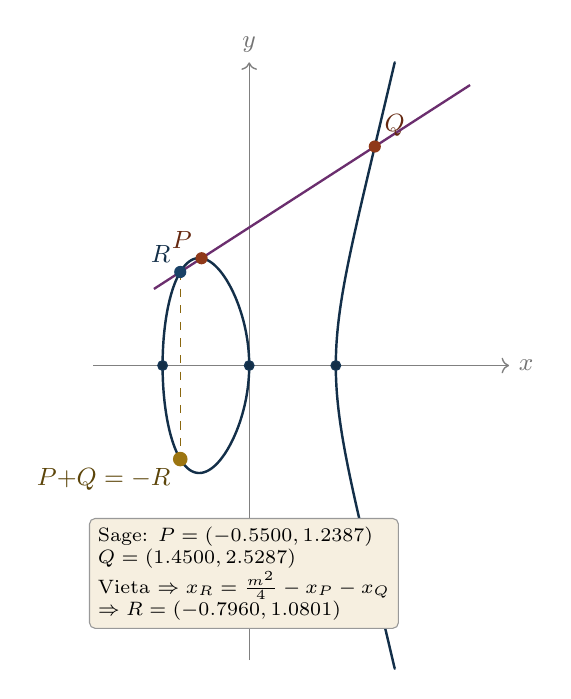
\begin{tikzpicture}[scale=1.1, every node/.style={font=\small}]
  % Axes
  \draw[->, black!50, line width=0.5pt] (-1.8,0) -- (3.0,0) node[right, black!55] {$x$};
  \draw[->, black!50, line width=0.5pt] (0,-3.4) -- (0,3.5) node[above, black!55] {$y$};
  % Sage curve y^2 = 4x^3 - 4x with roots -1, 0, 1
  % Curve arcs and branch points from sagemath/12_curve_sample.sage
  \drawprecisecurve
  % Roots
  \foreach \rt in {\rooteone,\rootetwo,\rootethree}
    \fill[formteal!60!black] (\rt,0) circle (1.3pt);
  % Sage-computed line through P, Q (passes through R = third intersection)
  \draw[draw=formplum, line width=0.85pt]
    (\chordlefta,\chordleftb) -- (\chordrighta,\chordrightb);
  % Vertical reflection line from R to -R
  \draw[dashed, line width=0.45pt, formgold!75!black]
    (\chordRx,\chordRy) -- (\chordSx,\chordSy);
  % Sage-computed points
  \fill[formrust!85!black] (\chordPx,\chordPy) circle (2pt);
  \node[formrust!60!black, above left] at (\chordPx,\chordPy) {$P$};
  \fill[formrust!85!black] (\chordQx,\chordQy) circle (2pt);
  \node[formrust!60!black, above right] at (\chordQx,\chordQy) {$Q$};
  \fill[formteal!85!black] (\chordRx,\chordRy) circle (2pt);
  \node[formteal!60!black, above left] at (\chordRx,\chordRy) {$R$};
  \fill[formgold!85!black] (\chordSx,\chordSy) circle (2.4pt);
  \node[formgold!50!black, below left] at (\chordSx,\chordSy) {$P{+}Q=-R$};
  % Annotation: sage-verified coordinates
  \node[draw=black!40, rounded corners=2pt, fill=formivory, align=left, anchor=west,
        inner sep=3pt, font=\scriptsize] at (-1.85,-2.4)
    {Sage: $P=(\chordPx,\chordPy)$\\
     $Q=(\chordQx,\chordQy)$\\
     Vieta $\Rightarrow x_R=\frac{m^2}{4}-x_P-x_Q$\\
     $\Rightarrow R=(\chordRx,\chordRy)$};
\end{tikzpicture}
\end{center}

\begin{keyidea}{Why the sign appears}
The line gives \(P+Q+R=O\), not \(P+Q=R\).  Therefore
\[
P+Q=-R.
\]
The final reflection is exactly this minus sign.
\end{keyidea}

\section{The Tangent Law: Doubling a Point}

\subsection{Intersection Multiplicity}

If \(P=Q\), the line through \(P\) and \(Q\) is replaced by the tangent line
at \(P\).  This is not a new rule.  It is the limiting case of the chord
rule as \(Q\to P\).

Algebraically, the tangent line has intersection multiplicity \(2\) at
\(P\).  If it meets the cubic again at \(R\), then
\[
L\cdot E=2P+R.
\]

\subsection{Divisor Argument}

Write
\[
P=\Phi(u),\qquad R=\Phi(w).
\]
The line divisor gives
\[
\left(\frac{\ell}{Z}\right)=2P+R-3O.
\]
Abel's sum law gives
\[
2u+w\equiv0\pmod{\Lambda}.
\]
Hence
\[
w\equiv-2u\pmod{\Lambda}.
\]
Therefore
\[
R=\Phi(-2u),
\]
and
\[
2P=\Phi(2u)=-R.
\]

\subsection{Geometric Rule}

To compute \(2P\):

\begin{enumerate}
\item Draw the tangent line to \(E\) at \(P\).
\item Let \(R\) be the third intersection with \(E\).
\item Reflect \(R\) across the \(x\)-axis.
\item The reflected point is \(2P\).
\end{enumerate}

\begin{center}
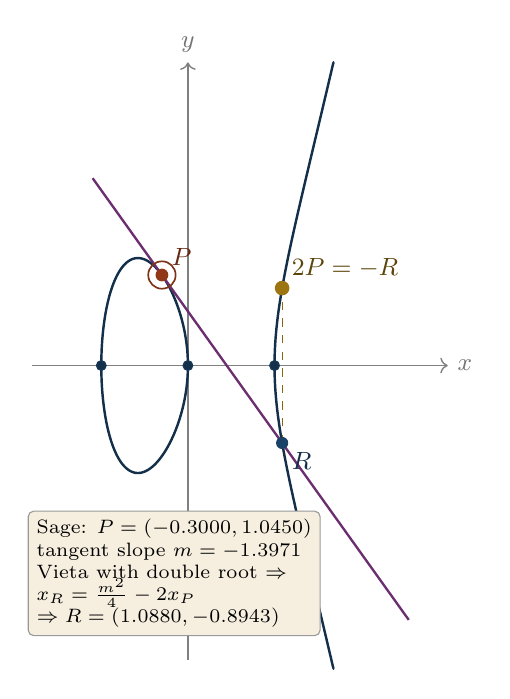
\begin{tikzpicture}[scale=1.1, every node/.style={font=\small}]
  \draw[->, black!50, line width=0.5pt] (-1.8,0) -- (3.0,0) node[right, black!55] {$x$};
  \draw[->, black!50, line width=0.5pt] (0,-3.4) -- (0,3.5) node[above, black!55] {$y$};
  % Sage curve y^2 = 4x^3 - 4x
  % Curve arcs and branch points from sagemath/12_curve_sample.sage
  \drawprecisecurve
  \foreach \rt in {\rooteone,\rootetwo,\rootethree}
    \fill[formteal!60!black] (\rt,0) circle (1.3pt);
  % Sage-computed tangent line at P
  \draw[draw=formplum, line width=0.85pt]
    (\dbllefta,\dblleftb) -- (\dblrighta,\dblrightb);
  % Reflection line
  \draw[dashed, line width=0.45pt, formgold!75!black]
    (\dblRx,\dblRy) -- (\dbltwoPx,\dbltwoPy);
  % P, R, 2P
  \fill[formrust!85!black] (\dblPx,\dblPy) circle (2.1pt);
  \node[formrust!60!black, above right] at (\dblPx,\dblPy) {$P$};
  \draw[draw=formrust!75!black, line width=0.6pt] (\dblPx,\dblPy) circle (4.5pt);
  \fill[formteal!85!black] (\dblRx,\dblRy) circle (2pt);
  \node[formteal!60!black, below right] at (\dblRx,\dblRy) {$R$};
  \fill[formgold!85!black] (\dbltwoPx,\dbltwoPy) circle (2.4pt);
  \node[formgold!50!black, above right] at (\dbltwoPx,\dbltwoPy) {$2P=-R$};
  % Annotation
  \node[draw=black!40, rounded corners=2pt, fill=formivory, align=left, anchor=west,
        inner sep=3pt, font=\scriptsize] at (-1.85,-2.4)
    {Sage: $P=(\dblPx,\dblPy)$\\
     tangent slope $m=\dblslope$\\
     Vieta with double root $\Rightarrow$\\
     $x_R=\tfrac{m^2}{4}-2x_P$\\
     $\Rightarrow R=(\dblRx,\dblRy)$};
\end{tikzpicture}
\end{center}

\section{The Identity, Inverses, and Vertical Lines}

\subsection{The Identity}

The identity element on the torus is \(0\).  Under the embedding,
\[
0\longmapsto O=[0:1:0].
\]
Therefore \(O\) is the identity on \(E\).

Geometrically, adding \(O\) should do nothing:
\[
P+O=P.
\]
This is compatible with the line rule.  A line through a finite point \(P\)
and \(O\) is the vertical line through \(P\).  It also passes through
\(-P\).  Thus
\[
P+O+(-P)=O,
\]
so
\[
P+O=P.
\]

\subsection{Vertical Lines}

Let
\[
P=(x,y).
\]
Then
\[
-P=(x,-y).
\]
The vertical line
\[
X=xZ
\]
passes through
\[
P,\quad -P,\quad O.
\]
The intersection divisor is
\[
P+(-P)+O.
\]
The line divisor gives
\[
P+(-P)+O-3O
=
P+(-P)-2O.
\]
Abel's sum law says
\[
P+(-P)+O=O
\]
in the group law, hence
\[
P+(-P)=O.
\]

\begin{center}
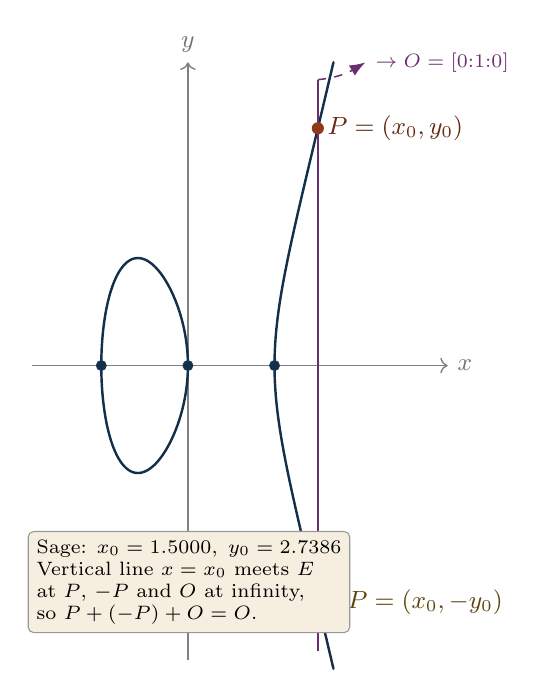
\begin{tikzpicture}[scale=1.1, every node/.style={font=\small}]
  \draw[->, black!50, line width=0.5pt] (-1.8,0) -- (3.0,0) node[right, black!55] {$x$};
  \draw[->, black!50, line width=0.5pt] (0,-3.4) -- (0,3.5) node[above, black!55] {$y$};
  % Curve arcs and branch points from sagemath/12_curve_sample.sage
  \drawprecisecurve
  \foreach \rt in {\rooteone,\rootetwo,\rootethree}
    \fill[formteal!60!black] (\rt,0) circle (1.3pt);
  % Sage-computed vertical line and the two intersections
  \draw[draw=formplum, line width=0.85pt] (\vertx,-3.3) -- (\vertx,3.3);
  \fill[formrust!85!black] (\vertx,\verty) circle (2pt);
  \node[formrust!60!black, right] at (\vertx,\verty) {$P=(x_0,y_0)$};
  \fill[formgold!85!black] (\vertx,{-\verty}) circle (2pt);
  \node[formgold!50!black, right] at (\vertx,{-\verty}) {$-P=(x_0,-y_0)$};
  \draw[draw=formplum, dashed, line width=0.55pt, -{Latex[length=2.0mm]}]
    (\vertx,3.3) to[bend right=14] ({\vertx+0.55},3.5);
  \node[formplum, font=\scriptsize, right] at ({\vertx+0.55},3.5) {$\to O=[0{:}1{:}0]$};
  \node[draw=black!40, rounded corners=2pt, fill=formivory, align=left, anchor=west,
        inner sep=3pt, font=\scriptsize] at (-1.85,-2.5)
    {Sage: $x_0=\vertx,\;y_0=\verty$\\
     Vertical line $x=x_0$ meets $E$\\
     at $P$, $-P$ and $O$ at infinity,\\
     so $P+(-P)+O=O$.};
\end{tikzpicture}
\end{center}

\subsection{Two-Torsion Points}

If \(P=-P\), then
\[
2P=O.
\]
In affine coordinates this means
\[
(x,y)=(x,-y),
\]
so
\[
y=0.
\]
Thus the nonzero two-torsion points are the points where the cubic crosses
the \(x\)-axis:
\[
4x^3-g_2x-g_3=0.
\]

At such a point, the tangent line is vertical, and the doubling rule gives
\[
2P=O.
\]

\begin{center}
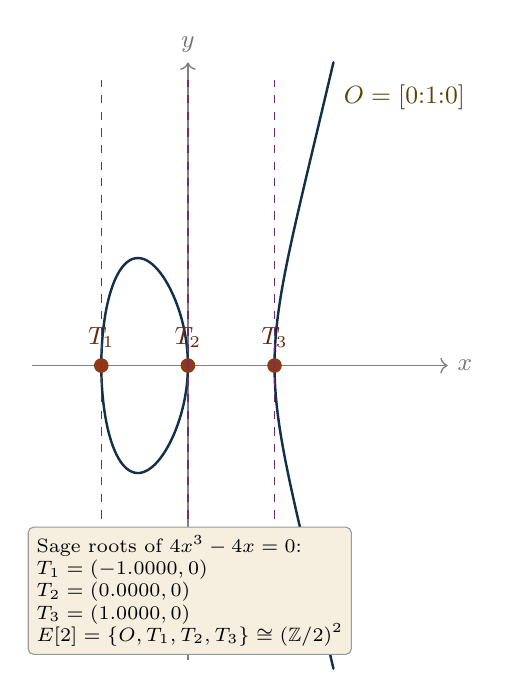
\begin{tikzpicture}[scale=1.1, every node/.style={font=\small}]
  \draw[->, black!50, line width=0.5pt] (-1.8,0) -- (3.0,0) node[right, black!55] {$x$};
  \draw[->, black!50, line width=0.5pt] (0,-3.4) -- (0,3.5) node[above, black!55] {$y$};
  % Curve arcs and branch points from sagemath/12_curve_sample.sage
  \drawprecisecurve
  % Sage-computed real 2-torsion x-coords
  \fill[formrust!85!black] (\torstwoone,0) circle (2.4pt);
  \node[formrust!60!black, above] at (\torstwoone,0.10) {$T_1$};
  \fill[formrust!85!black] (\torstwotwo,0) circle (2.4pt);
  \node[formrust!60!black, above] at (\torstwotwo,0.10) {$T_2$};
  \fill[formrust!85!black] (\torstwothree,0) circle (2.4pt);
  \node[formrust!60!black, above] at (\torstwothree,0.10) {$T_3$};
  % Vertical tangents at the roots
  \draw[draw=formplum, dashed, line width=0.5pt] (\torstwoone,-3.3) -- (\torstwoone,3.3);
  \draw[draw=formplum, dashed, line width=0.5pt] (\torstwotwo,-3.3) -- (\torstwotwo,3.3);
  \draw[draw=formplum, dashed, line width=0.5pt] (\torstwothree,-3.3) -- (\torstwothree,3.3);
  \node[formgold!50!black, font=\small] at (2.5,3.1) {$O=[0{:}1{:}0]$};
  \node[draw=black!40, rounded corners=2pt, fill=formivory, align=left, anchor=west,
        inner sep=3pt, font=\scriptsize] at (-1.85,-2.6)
    {Sage roots of $4x^3-4x=0$:\\
     $T_1=(\torstwoone,0)$\\
     $T_2=(\torstwotwo,0)$\\
     $T_3=(\torstwothree,0)$\\
     $E[2]=\{O,T_1,T_2,T_3\}\cong(\Z/2)^2$};
\end{tikzpicture}
\end{center}

\section{Coordinate Formulas for the Group Law}

The divisor proof explains why the chord--tangent construction is correct.
It is also useful to have explicit formulas.

\subsection{Addition of Distinct Noninverse Points}

Let
\[
P=(x_1,y_1),
\qquad
Q=(x_2,y_2)
\]
be finite points on
\[
E:\quad y^2=4x^3-g_2x-g_3.
\]
Assume
\[
P\neq Q,
\qquad
Q\neq -P.
\]
Then \(x_1\neq x_2\), and the slope of the line through \(P\) and \(Q\) is
\[
m=\frac{y_2-y_1}{x_2-x_1}.
\]
The line is
\[
y=mx+b,
\qquad
b=y_1-mx_1.
\]

Substitute this into the cubic:
\[
(mx+b)^2=4x^3-g_2x-g_3.
\]
Rearrange:
\[
4x^3-m^2x^2-(g_2+2mb)x-(g_3+b^2)=0.
\]
The roots are the \(x\)-coordinates of the three intersection points:
\[
x_1,\quad x_2,\quad x_R.
\]
By Vieta's formula,
\[
x_1+x_2+x_R=\frac{m^2}{4}.
\]
Thus
\[
x_R=\frac{m^2}{4}-x_1-x_2.
\]

Since
\[
P+Q=-R,
\]
the \(x\)-coordinate of \(P+Q\) is the same:
\[
\boxed{
x_{P+Q}=\frac{m^2}{4}-x_1-x_2.
}
\]
The \(y\)-coordinate is the negative of the line value at \(x_R\):
\[
\boxed{
y_{P+Q}=-(mx_{P+Q}+b).
}
\]

\subsection{Doubling Formula}

For
\[
P=(x_1,y_1)
\]
with \(y_1\neq0\), the tangent slope is found by implicit differentiation.
Starting from
\[
y^2=4x^3-g_2x-g_3,
\]
differentiate:
\[
2y\frac{dy}{dx}=12x^2-g_2.
\]
Therefore
\[
m=\frac{dy}{dx}\bigg|_P
=
\frac{12x_1^2-g_2}{2y_1}.
\]
Then the same formulas apply:
\[
\boxed{
x_{2P}=\frac{m^2}{4}-2x_1,
}
\]
and
\[
\boxed{
y_{2P}=-(mx_{2P}+b),
\qquad
b=y_1-mx_1.
}
\]

\subsection{Special Cases}

\begin{center}
\begin{tabular}{c|c}
Situation & Result\\
\hline
\(P=O\) & \(P+Q=Q\)\\
\(Q=O\) & \(P+Q=P\)\\
\(Q=-P\) & \(P+Q=O\)\\
\(P=Q,\ y_P=0\) & \(2P=O\)\\
\(P=Q,\ y_P\neq0\) & use tangent formula
\end{tabular}
\end{center}

\section{Analytic Addition Formula for \texorpdfstring{\(\wp\)}{wp}}

\subsection{The Formula}

The Weierstrass addition formula says
\[
\boxed{
\wp(u+v)
=
-\wp(u)-\wp(v)
+
\frac14
\left(
\frac{\wp'(u)-\wp'(v)}{\wp(u)-\wp(v)}
\right)^2
}
\]
whenever the expression is defined; the exceptional cases follow by limits.

Let
\[
P=\Phi(u)=(\wp(u),\wp'(u)),
\qquad
Q=\Phi(v)=(\wp(v),\wp'(v)).
\]
Set
\[
x_1=\wp(u),\quad y_1=\wp'(u),
\qquad
x_2=\wp(v),\quad y_2=\wp'(v).
\]
The slope of the chord is
\[
m=\frac{y_2-y_1}{x_2-x_1}
=
\frac{\wp'(v)-\wp'(u)}{\wp(v)-\wp(u)}.
\]
This equals
\[
\frac{\wp'(u)-\wp'(v)}{\wp(u)-\wp(v)}
\]
after multiplying numerator and denominator by \(-1\).

The coordinate formula from the chord computation gives
\[
x_{P+Q}
=
\frac{m^2}{4}-x_1-x_2.
\]
The addition formula gives exactly
\[
\wp(u+v)
=
\frac{m^2}{4}-\wp(u)-\wp(v).
\]
Thus
\[
x_{P+Q}=\wp(u+v).
\]

\subsection{\texorpdfstring{Why the \(y\)-Coordinate Has the Reflected Sign}{Why the y-Coordinate Has the Reflected Sign}}

The third intersection point is
\[
R=\Phi(-(u+v)).
\]
Its coordinates are
\[
R=(\wp(-(u+v)),\wp'(-(u+v))).
\]
Since \(\wp\) is even and \(\wp'\) is odd,
\[
R=(\wp(u+v),-\wp'(u+v)).
\]
Therefore
\[
-R=(\wp(u+v),\wp'(u+v)).
\]
But
\[
\Phi(u+v)=(\wp(u+v),\wp'(u+v)).
\]
Hence
\[
P+Q=\Phi(u+v)=-R.
\]

\begin{keyidea}{Analytic and geometric agreement}
The addition formula for \(\wp\) is the analytic version of the chord law.
The root-sum calculation gives the same \(x\)-coordinate as
\(\wp(u+v)\), and the oddness of \(\wp'\) supplies the reflection.
\end{keyidea}

\section{Why the Chord--Tangent Law Is Forced}

We can now isolate the exact logical mechanism.

\subsection{There Is Already a Group Law}

The torus \(T=\C/\Lambda\) already has an abelian group law:
\[
[u]+[v]=[u+v].
\]
There is no choice here.  It comes directly from addition in \(\C\).

\subsection{\texorpdfstring{The \(\wp\)-Embedding Transfers That Law}{The wp-Embedding Transfers That Law}}

The map
\[
\Phi:T\to E
\]
identifies the torus with the cubic.  Therefore it transports the group law:
\[
P+_E Q
=
\Phi(\Phi^{-1}(P)+\Phi^{-1}(Q)).
\]
Again, there is no choice if we require \(\Phi\) to be a group
isomorphism.

\subsection{Lines Know the Same Group Law}

For every projective line \(L\),
\[
L\cdot E=P+Q+R
\]
and
\[
P+Q+R-3O
\]
is principal.  Abel's sum law says principal divisors have group sum zero.
Therefore
\[
P+Q+R=O.
\]
Solving for \(P+Q\) gives
\[
P+Q=-R.
\]

\subsection{The Result}

\begin{theorem}
Under the Weierstrass embedding
\[
\Phi:\C/\Lambda\to E,\qquad z\mapsto[\wp(z):\wp'(z):1],
\]
the abelian group law on \(\C/\Lambda\) becomes the chord--tangent group law
on
\[
E:\quad Y^2Z=4X^3-g_2XZ^2-g_3Z^3.
\]
\end{theorem}

\begin{proof}
Let \(P=\Phi(u)\) and \(Q=\Phi(v)\).  If \(P,Q\) are distinct and not
inverse, let the line through them meet \(E\) again at \(R=\Phi(w)\).  The
line divisor gives the principal divisor
\[
P+Q+R-3O.
\]
By Abel's sum law,
\[
u+v+w\equiv0\pmod{\Lambda}.
\]
Thus
\[
w\equiv-(u+v).
\]
Therefore
\[
R=\Phi(-(u+v)).
\]
Reflecting gives
\[
-R=\Phi(u+v),
\]
which is the transported torus sum of \(P\) and \(Q\).  The tangent,
vertical-line, and identity cases are the same argument with intersection
multiplicities.  Hence the transported group law is exactly the
chord--tangent law.
\end{proof}

\begin{keyidea}{No arbitrary convention}
The chord--tangent rule is forced by three facts:
\[
\text{torus addition}
\quad+\quad
\wp\text{-embedding}
\quad+\quad
\text{principal line divisors}.
\]
The reflection step is forced because the line gives
\[
P+Q+R=O,
\]
so the desired sum is \(-R\).
\end{keyidea}

\section{A Complete Worked Symbolic Computation}

This section performs the chord computation from beginning to end in
coordinates.

\subsection{Start with Two Points}

Let
\[
P=(x_1,y_1),
\qquad
Q=(x_2,y_2)
\]
on
\[
y^2=4x^3-g_2x-g_3.
\]
Assume \(x_1\neq x_2\).  Define
\[
m=\frac{y_2-y_1}{x_2-x_1},
\qquad
b=y_1-mx_1.
\]
The chord is
\[
y=mx+b.
\]

\subsection{Substitute}

Plug into the cubic:
\[
(mx+b)^2=4x^3-g_2x-g_3.
\]
Move everything to one side:
\[
4x^3-m^2x^2-(g_2+2mb)x-(g_3+b^2)=0.
\]
Since \(P\) and \(Q\) lie on both the line and the cubic, \(x_1\) and \(x_2\)
are roots.  Let the third root be \(x_3\).  Then
\[
4(x-x_1)(x-x_2)(x-x_3)
\]
has the same leading coefficient and the same roots.  Comparing the
\(x^2\)-coefficient:
\[
-4(x_1+x_2+x_3)=-m^2.
\]
Therefore
\[
x_3=\frac{m^2}{4}-x_1-x_2.
\]

\subsection{Find the Third Point and Reflect}

The third intersection point is
\[
R=(x_3,y_3),
\qquad
y_3=mx_3+b.
\]
The group sum is
\[
P+Q=-R.
\]
Since inverse is reflection,
\[
-R=(x_3,-y_3).
\]
Therefore
\[
\boxed{
P+Q=
\left(
\frac{m^2}{4}-x_1-x_2,\;
-m\left(\frac{m^2}{4}-x_1-x_2\right)-b
\right).
}
\]

\subsection{\texorpdfstring{Comparison with the More Common Cubic \(y^2=x^3+ax+b\)}{Comparison with the More Common Cubic y2=x3+ax+b}}

Many textbooks use
\[
y^2=x^3+ax+b.
\]
In that normalization, the addition formula is
\[
x_{P+Q}=m^2-x_1-x_2.
\]
Our cubic is
\[
y^2=4x^3-g_2x-g_3.
\]
The leading coefficient is \(4\), so Vieta's formula gives
\[
x_{P+Q}=\frac{m^2}{4}-x_1-x_2.
\]
The factor \(1/4\) is not mysterious; it comes from the coefficient of
\(x^3\).

\section{Common Pitfalls and How to Avoid Them}

\begin{enumerate}
\item \textbf{Forgetting the point at infinity.}
The cubic group law is not complete unless \(O=[0:1:0]\) is included.
Vertical lines meet the cubic at \(O\), and \(O\) is the identity.

\item \textbf{Saying the third intersection is \(P+Q\).}
The third intersection is \(R\), but the sum is \(-R\).  The line gives
\[
P+Q+R=O.
\]

\item \textbf{Ignoring multiplicity.}
When \(P=Q\), the tangent line counts \(P\) twice:
\[
L\cdot E=2P+R.
\]
When the tangent has higher contact, the same divisor rule still applies.

\item \textbf{Treating reflection as a visual trick.}
Reflection is the inverse map on the torus:
\[
z\mapsto -z.
\]
It becomes
\[
(x,y)\mapsto(x,-y)
\]
because \(\wp\) is even and \(\wp'\) is odd.

\item \textbf{Using Riemann--Roch without checking genus.}
The dimension counts
\[
\ell(nO)=n
\]
depend on the fact that the torus has genus \(1\) and \(K\sim0\).

\item \textbf{Confusing affine and projective equations.}
The affine equation
\[
y^2=4x^3-g_2x-g_3
\]
misses the point \(O\).  The correct compact curve is
\[
Y^2Z=4X^3-g_2XZ^2-g_3Z^3.
\]
\end{enumerate}

\section{Lecture Summary}

The complete chain is:

\begin{enumerate}
\item A lattice \(\Lambda\subset\C\) gives a compact genus-one Riemann
surface
\[
T=\C/\Lambda.
\]

\item The torus has an intrinsic abelian group law:
\[
[u]+[v]=[u+v].
\]

\item Riemann--Roch on a genus-one surface says the first nonconstant
meromorphic function with one pole has a double pole.  This is \(\wp\).

\item The functions
\[
1,\wp,\wp'
\]
span \(L(3O)\), so they define a map
\[
\Phi:T\to\CP^2.
\]

\item The differential equation
\[
(\wp')^2=4\wp^3-g_2\wp-g_3
\]
shows that the image is the cubic
\[
E:\quad Y^2Z=4X^3-g_2XZ^2-g_3Z^3.
\]

\item The point \(0\in T\) maps to
\[
O=[0:1:0].
\]

\item The inverse map \(z\mapsto -z\) becomes
\[
(x,y)\mapsto(x,-y).
\]

\item A line \(L\) cuts the cubic in
\[
P+Q+R.
\]
Since \(Z=0\) cuts the cubic in \(3O\), the divisor
\[
P+Q+R-3O
\]
is principal.

\item Principal divisors on a torus have Abel sum zero.  Therefore
\[
P+Q+R=O.
\]

\item Hence
\[
P+Q=-R,
\]
which is exactly the chord--tangent law.
\end{enumerate}

\begin{keyidea}{Final takeaway}
The chord--tangent law is the visible projective shadow of the simple
addition law
\[
[u]+[v]=[u+v]
\]
on the complex torus.  The Weierstrass embedding turns addition into line
intersection because line intersections give principal divisors, and
principal divisors have zero Abel sum.
\end{keyidea}

\end{document}
